% Free range VHDL
% Authors: Bryan Mealy, Fabrizio Tappero
% Date: May, 2012
% URL: freerangefactory.org
% (C) 2012 B. Mealy, F. Tappero
%
% !TEX root = master.tex
%
%\documentclass[11pt,b5paper]{book} % you can set the paper size in style.sty
%\documentclass[gray, 11pt,b5paper]{book} % generate whole document in B&W
\documentclass[11pt,b5paper]{book} % generate whole document in color
\usepackage{style}


% LINE SPACING
\renewcommand{\baselinestretch}{1.2} % custom spacing
%\renewcommand{\baselinestretch}{2} % double-line spacing

%%%%%% DOCUMENT BEGIN %%%%%%
\begin{document}

	% front cover
	\thispagestyle{empty}
	\begin{textblock*}{160mm}(-3mm,0mm)
	%\textblockcolour{red}
    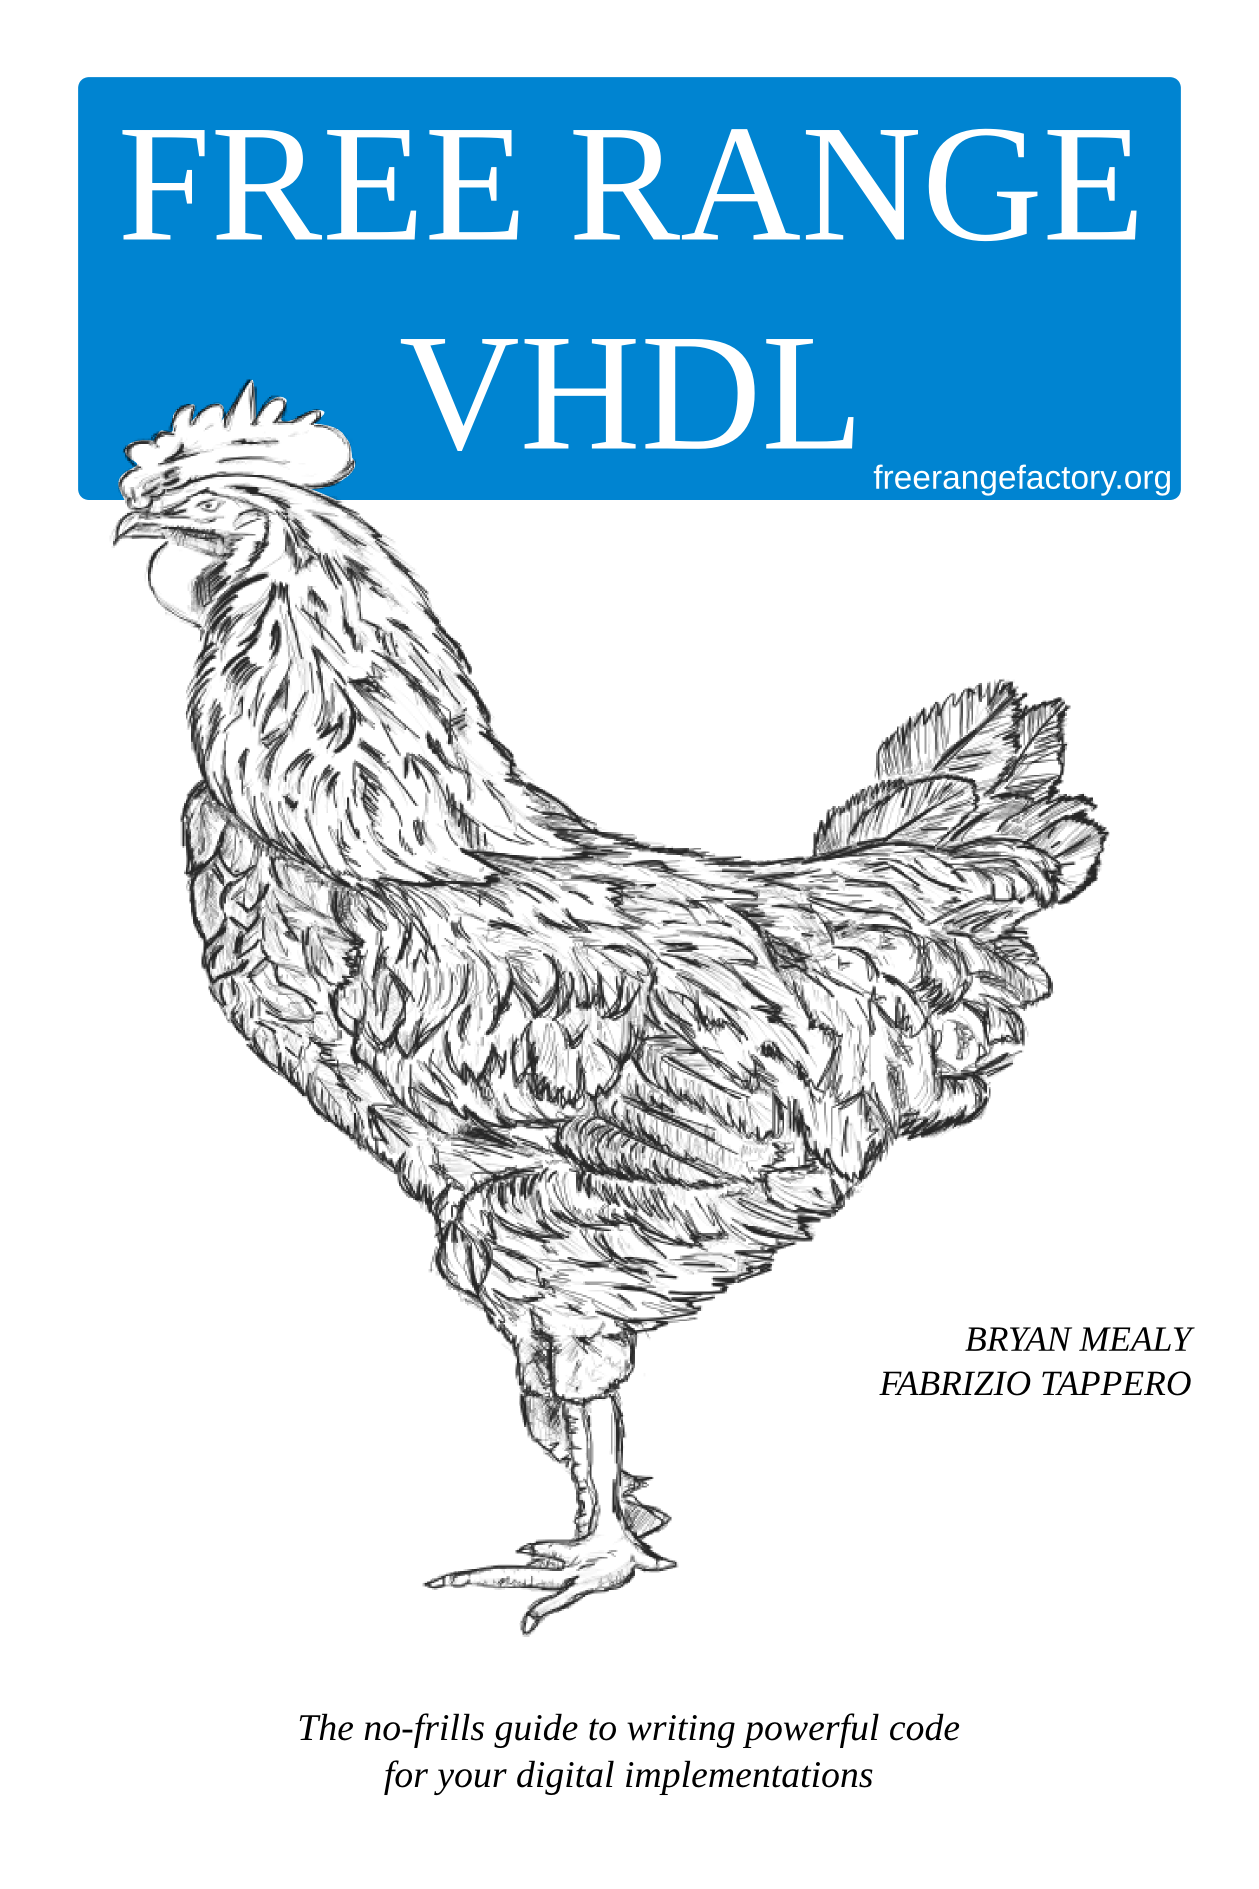
\includegraphics[width=160mm]{pics/cover.png}  % full-page picture for 160x240 format
	\end{textblock*}
	\null\newpage % latex might neglect \newpage because the page is empty, 

	% blank page
	\thispagestyle{empty}
	\null\newpage

	% front matter %
	\thispagestyle{empty}
	\begin{textblock*}{60mm}(85mm,90mm)
	%\textblockcolour{red}
	\noindent
	{\sffamily\LARGE\bfseries Free Range VHDL}\\
	\noindent
	{\sffamily\small Bryan Mealy, Fabrizio Tappero}\\
	{\color{dark-gray}\rule[5pt]{170pt}{3pt}}
	\end{textblock*}
	\null\newpage

	% license page %
	\thispagestyle{empty}
	% Free range VHDL
% Authors: Bryan Mealy, Fabrizio Tappero
% Date: May, 2012
% URL: freerangefactory.org
% (C) 2012 B. Mealy, F. Tappero
%
% !TEX root = master.tex
%
\setcounter{page}{1}

{\footnotesize
\noindent
Free Range VHDL\\
Copyright \copyright 2012 B. Mealy, F. Tappero\\
Release: 1.14\\
Date: \today\\
Book size: 160 mm by 240 mm\\
Pages: approx. 190\\
\vspace{20pt}

\noindent
The electronic version of this book can be downloaded free of charge from:

\noindent
\url{http://www.freerangefactory.org}

\vspace{15pt}

\noindent
The authors have taken great care in the preparation of this book, but make no expressed or implied warranty of any kind and assume no responsibility for errors or omissions. No liability is assumed for incidental or consequential damages in connection with or arising out of the use of the information or programs contained in this book.\\

\noindent
This book is licensed under the Creative Commons Attribution-ShareAlike Unported License, which permits unrestricted use, distribution, adaptation and reproduction in any medium, provided the original work is properly cited. If you build upon this work, you may distribute the resulting work only under the same, similar or a compatible license. To view a copy of this license, visit:

\noindent
\url{http://creativecommons.org/licenses/by-sa/3.0/}
\vspace{25pt}

\noindent
{\sffamily\bfseries Feedback and Contribution}

\noindent
We are more than happy to consider your contribution in improving, extending or correcting any part of this book.
For any communication or feedback that you might have about the content of this book you can contact the authors at the following address:

\noindent
\texttt{contact@freerangefactory.org}\\

\vfill
\noindent
Cover and Artwork by Robert Ash.

} % close footnotsize environment


	% blank page with note
	\thispagestyle{empty}
	\null
	\vspace*{\fill}
	\begin{center}\textit{To everyone who helped}\end{center}
	\vspace*{\fill}
	\newpage

	% blank page
	\thispagestyle{empty}
	\null\newpage

	% table of contents page %
	\setcounter{page}{5}
	\renewcommand\contentsname{Table of Contents} % rename title
	\pagenumbering{roman}
	\tableofcontents
	%\null\newpage

	% Acknowledgments, from page i
	% Free range VHDL
% Authors: Bryan Mealy, Fabrizio Tappero
% Date: May, 2012
% URL: freerangefactory.org
% (C) 2012 B. Mealy, F. Tappero
%
% !TEX root = master.tex
%
\addcontentsline{toc}{chapter}{Acknowledgments}
\chapter*{Acknowledgments}
The authors would like to thank Christina Jarron for her invaluable contribution to proofreading this book and for her useful suggestions. Special thanks also to Rob Ash for helping us make the cover of the book distinctive with his original artwork. A massive thank you goes to Keith Knowles for his time and effort in reviewing and editing the final draft of this book. Finally, the authors would like to thank all the people who have provided feedback and suggestions.



	% blank page
	\thispagestyle{empty}
	\null\newpage

	% Preface, from page ii
	\setcounter{page}{1}
	\pagenumbering{arabic}
	% Free range VHDL
% Authors: Bryan Mealy, Fabrizio Tappero
% Date: May, 2011
%
% (C) 2011 B. Mealy, F. Tappero
%
% !TEX root = master.tex
%
\phantomsection
\addcontentsline{toc}{chapter}{Purpose of this book} % add chapter*{Purpose of this book}
\chapter*{Purpose of this book}
The purpose of this book is to provide students and young engineers with a guide to help them develop the skills necessary to be able to use VHDL for introductory and intermediate level digital design. These skills will also give you the ability and the confidence to continue on with VHDL-based digital design. In this way, you will also take steps toward developing the skills required to implement more advanced digital design systems.
Although there are many books and on-line tutorials dealing with VHDL, these sources are often troublesome for several reasons. Firstly, much of the information regarding VHDL is either needlessly confusing or poorly written. Material with these characteristics seems to be written from the standpoint of someone who is either painfully intelligent or has forgotten that their audience may be seeing the material for the first time. Secondly, the common approach for most VHDL manuals is to introduce too many topics and a lot of extraneous information too early. Most of this material would best appear later in the presentation. Material presented in this manner has a tendency to be confusing, is easily forgotten if misunderstood or simply is never applied. The approach taken by this book is to provide only what you need to know to quickly get up and running in VHDL. As with all learning, once you have obtained and applied some useful information, it is much easier to build on what you know as opposed to continually adding information that is not directly applicable to the subjects at hand.

The intent of this book is to present topics to someone familiar with digital logic design and with some skills in algorithmic programming languages such as Java or C. The information presented here is focused on giving a solid knowledge of the approach and function of VHDL. With a logical and intelligent introduction to basic VHDL concepts, you should be able to quickly and efficiently create useful VHDL code. In this way, you will see VHDL as a valuable design, simulation and test tool rather than another batch of throw-away technical knowledge encountered in some forgotten class or lab.

Lastly, VHDL is an extremely powerful tool. The more you understand as you study and work with VHDL, the more it will enhance your learning experience independently of your particular area of interest. It is well worth noting that VHDL and other similar hardware design languages are used to create most of the digital integrated circuits found in the various electronic gizmos that overwhelm our modern lives. The concept of using software to design hardware that is controlled by software will surely provide you with endless hours of contemplation. VHDL is a very exciting language and mastering it will allow you to implement systems capable of handling and processing in parallel ns-level logic events in a comfortable software environment.

This book was written with the intention of being freely available to everybody. The formatted electronic version if this book is available from the Internet. Any part of this book can be copied, distributed and modified in accordance with the conditions of its license.
\vspace{10pt}

\noindent
\textbf{DISCLAIMER:}
This book quickly takes you down the path toward understanding VHDL and writing solid VHDL code. The ideas presented herein represent the core knowledge you will need to get up and running with VHDL. This book in no way presents a complete description of the VHDL language. In an effort to expedite the learning process, some of the finer details of VHDL have been omitted from this book. Anyone who has the time and inclination should feel free to further explore the true depth of the VHDL language. There are many on-line VHDL reference books and free tutorials. If you find yourself becoming curious about what this book is not telling you about VHDL, take a look at some of these references.



	% from page 1 begins Chapter 1 %
	% Freerange VHDL
% Authors: Bryan Mealy, Fabrizio Tappero
% Date: May, 2011
%
% (C) 2011 B. Mealy, F. Tappero
%
% !TEX root = !TEX root = master.tex.tex
%
\chapter{Introduction To VHDL}
VHDL has a rich and interesting history\footnote{VHDL-Wikipedia: \url{http://en.wikipedia.org/wiki/VHDL}}. But since knowing this history is probably not going to help you write better VHDL code, it will only be briefly mentioned here. Consulting other, lengthier texts or search engines will provide more information for those who are interested. Regarding the VHDL acronym,  the V is short for yet another acronym: VHSIC or Very High-Speed Integrated Circuit. The HDL stands for Hardware Description Language. Clearly, the state of technical affairs these days has done away with the need for nested acronyms. VHDL is a true computer language with the accompanying set of syntax and usage rules. But, as opposed to higher-level computer languages, VHDL is primarily used  to \textit{describe hardware}. The tendency for most people familiar with a higher-level computer language such as C or Java is to view VHDL as just another computer language. This is not altogether a bad approach if such a view facilitates the understanding and memorisation of the language syntax and structure. The common mistake made by someone with this approach is to attempt to program in VHDL as they would program a higher-level computer language. Higher-level computer languages are sequential in nature; VHDL is not. 

VHDL was invented to describe hardware and in fact VHDL is a \textit{concurrent} language. What this means is that, normally, VHDL instructions are all executed at the same time (concurrently), regardless of the size of your implementation. Another way of looking at this is that higher-level computer languages are used to describe algorithms (sequential execution) and VHDL is used to describe hardware (parallel execution). This inherent difference should necessarily encourage you to re-think how you write your VHDL code. Attempts to write VHDL code with a high-level language style generally results in VHDL code that no one understands. Moreover, the tools used to synthesize\footnote{Synthesis: the process of programming a device like a FPGA or a CPLD} this type of code have a tendency to generate circuits that generally do not work correctly and have bugs that are nearly impossible to trace. And if the circuit does actually work, it will most likely be inefficient due to the fact that the resulting hardware was unnecessarily large and overly complex. This problem is compounded as the size and complexity of your circuits becomes greater.

There are two primary purposes for hardware description languages such as VHDL. First, VHDL can be used to model digital circuits and systems. Although the word ``model'' is one of those overly used words in engineering, in this context it simply refers to a description of something that presents a certain level of detail. The nice thing about VHDL is that the level of detail is unambiguous due to the rich syntax rules associated with it. In other words, VHDL provides everything that is necessary in order to describe any digital circuit. Likewise, a digital circuit/system is any circuit that processes or stores digital information. Second, having some type of circuit model allows for the subsequent simulation and/or testing of the circuit. The VHDL model can also be translated into a form that can be used to generate actual working circuits. The VHDL model is magically\footnote{It is not really magic. There is actually a well-defined science behind it.} interpreted by software tools in such a way as to create actual digital circuits in a process known as \textit{synthesis}.

There are other logic languages available to model the behaviour of digital circuit designs that are easy to use because they provide a graphical method to model circuits. For them, the tendency is to prefer the graphical approach because it has such a comfortable learning curve. But, as you can easily imagine, your growing knowledge of digital concepts is accompanied by the ever-increasing complexity of digital circuits you are dealing with. The act of graphically connecting a bunch of lines on the computer screen quickly becomes tedious. The more intelligent approach to digital circuit design is to start with a system that is able to describe exactly how your digital circuit works (in other words, modelling it) without having to worry about the details of connecting massive quantities of signal lines. Having a working knowledge of VHDL will provide you with the tools to model digital circuits in a much more intelligent manner.

Finally, you will be able to use your VHDL code to create actual functioning circuits. This allows you to implement relatively complex circuits in a relatively short period of time. The design methodology you will be using allows you to dedicate more time to designing your circuits and less time ``constructing'' them. The days of placing, wiring, and troubleshooting multiple integrated circuits on a proto-board are gone.

VHDL is a very exciting language that can allow the design and implementation of functions capable of processing an enormous amount of data by employing a relatively low-cost and low-power hardware. Moreover, what is really impressive is that, via simple VHDL modules, you can have direct access to basic ns-level logic events as well as communicate using a USB port or drive a VGA monitor to visualise graphics of modest complexity.

Modelling digital circuits with VHDL represents a modern digital design paradigm where the programmer writes in a descriptive manner a description of what the final logic circuit should do and a, hopefully intelligent, language compiler, in this case called synthesizer, attempts to ``infer'' what the actual final physical logic circuit should be. The direct consequence of it, is that novice programmers do not generally seem able to convince the synthesizer to implement what seems very clear in their mind.
A some how old-fashion alternative method to a descriptive language approach is a scenario where the programmer simply interconnects a finite number of digital blocks, that he pools from a library, in the attempt to reach the same objective. This approach is not only very time consuming but also inherently limiting and very error prone.
Modern digital design is more about appropriately modelling digital circuits and maintaining a quality description of the circuit. All that is left now is learning the description language and the associated digital design paradigm.

\section{Golden Rules of VHDL}
Before you start, here are a couple of points that you should never forget when working with VHDL.\\

\noindent
\textbf{VHDL is a hardware-design language.} Although most people have probably already been exposed to some type of higher-level computer language, these skills are only indirectly applicable to VHDL. When you are working with VHDL, you are not programming, you are ``designing hardware''. Your VHDL code should reflect this fact. What does this mean? It means that unless you are inside certain constructs, your code lines will be executed almost all at once. If your VHDL code appears too similar to code of a higher-level computer language, it is probably bad VHDL code. This is vitally important.\\

\noindent
\textbf{Have a general concept of what your hardware should look like.} Although VHDL is vastly powerful, if you do not understand basic digital constructs, you will probably be unable to generate efficient digital circuits. Digital design is similar to higher-level language programming in that even the most complicated programming at any level can be broken down into some simple programming constructs. There is a strong analogy to digital design in that even the most complicated digital circuits can be described in terms of basic digital constructs. In other words, if you are not able to roughly envision the digital circuit you are trying to model in terms of basic digital circuits, you will probably misuse VHDL, thus angering the VHDL gods. VHDL is cool, but it is not as magical as it initially appears to be.

\section{Tools Needed for VHDL Development}
VHDL is a programming language used to implement hardware which will run other software (for example C). A Field Programmable Gate Array (FPGA) is probably the most common device that you can use for your VHDL implementations. If you want to do VHDL coding for FPGAs you will have to play with the rules that current major FPGA manufacturers have drawn up to help you (rules which also ensure their continued existence on the market).

The successful implementation of a VHDL-based system roughly calls for the following steps: VHDL code writing, compiling, simulation and synthesis. All major FPGA manufacturers have a set of software and hardware tools that you can use to perform the mentioned steps. Most of these software tools are free of charge but are not open-source. Nevertheless, the same tools follow a license scheme, whereby paying a certain amount of money allows you to take advantage of sophisticated software features or get your hands on proprietary libraries with lots of components (e.g. a 32-bit processor) that you can easily include in your own project. 

If your have no interest in proprietary libraries you can use open-source solutions (e.g. GHDL\footnote{Open-source VHDL simulator GHDL: \url{http://ghdl.free.fr}}) which will allow you to compile and simulate your VHDL code using the open-source tool \textit{gcc\footnote{Multi-language open-source compiler GCC: \url{http://gcc.gnu.org}}}. At the time of writing, no open-source solution is available for the synthesis process. However synthesis can be accomplished using a free-license version of any major FPGA manufacturer's software tool (e.g. Xilinx ISE Design Suite).

Thanks to the open-source community, you can write, compile and simulate VHDL systems using excellent open-source solutions. This book will show you how to get up and running with the VHDL language. For the further tasks like synthesis and upload of your code into an FPGA, the free of charge Xilinx ISE Design Suite\footnote{Xilinx ISE Design Suite: \url{http://www.xilinx.com/tools/designtools.htm}} or the Altera equivalent tool Quartus, can be employed.

 


	% Free range VHDL
% Authors: Bryan Mealy, Fabrizio Tappero
% Date: May, 2012
% URL: freerangefactory.org
% (C) 2012 B. Mealy, F. Tappero
%
% !TEX root = master.tex
%
\chapter{VHDL Invariants}
There are several features of VHDL that you should know before moving forward. Although it is rarely a good idea for people to memorize anything, you should memorize the basic concepts presented in this section. This should help eliminate some of the drudgery involved in learning a new programming language and lay the foundation that will enable you to create visually pleasing and good VHDL source code.

\section{Case Sensitivity}
\textbf{VHDL is not case sensitive}. This means that the two statements shown in Listing \ref{case_sens} have the exact same meaning (don't worry about what the statement actually means though). Keep in mind that Listing \ref{case_sens} shows an example of VHDL case sensitivity and not good VHDL coding practices.

\noindent
\begin{minipage}{0.99\linewidth}
\begin{lstlisting}[label=case_sens, caption=An example of VHDL case insensitivity.]
Dout <= A and B;								doUt <= a AnD b;
\end{lstlisting}
\end{minipage}

\section{White Space}
\textbf{VHDL is not sensitive to white space} (spaces and tabs) in the source document. The two statements in Listing \ref{white_spaces} have the exact same meaning. Once again, Listing \ref{white_spaces} is not an example of good VHDL coding style. Note that Listing \ref{white_spaces} once again indicates that VHDL is not case sensitive.

\noindent
\begin{minipage}{0.99\linewidth}
\begin{lstlisting}[label=white_spaces, caption=An example showing VHDL's indifference to white space.]
nQ <= In_a or In_b;						nQ   <=in_a OR       in_b;
\end{lstlisting}
\end{minipage}

\section{Comments}
Comments in VHDL begin with the symbol ``\texttt{--}'' (two consecutive dashes). The VHDL synthesizer ignores anything after the two dashes and up to the end of the line in which the dashes appear. Listing \ref{comments} shows two types of commenting styles. Unfortunately, there are no block-style comments (comments that span multiple lines but do not require comment marks on every line) available in VHDL.

\noindent
\begin{minipage}{0.99\linewidth}
\begin{lstlisting}[label=comments, caption=Two typical uses of comments.]
-- This next section of code is used to blah-blah
-- This type of comment is the best fake for block-style commenting.
PS_reg <= NS_reg; -- Assign next_state value to present_state
\end{lstlisting}
\end{minipage}

Appropriate use of comments increases both the readability and the understandability of VHDL code. The general rule is to comment any line or section of code that may not be clear to a reader of your code besides yourself. The only inappropriate use of a comment is to state something that is patently obvious. It is hard to imagine code that has too few comments so don't be shy: use lots of comments. Research has shown that using lots of appropriate comments is actually a sign of high intelligence.

\section{Parentheses}
VHDL is relatively lax on its requirement for using parentheses. Like other computer languages, there are a few precedence rules associated with the various operators in the VHDL language. Though it is possible to learn all these rules and write clever VHDL source code that will ensure the readers of your code are left scratching their heads, a better idea is to practice liberal use of parentheses to ensure the human reader of your source code understands the purpose of the code. Once again, the two statements appearing in Listing \ref{parenthesis} have the same meaning. Note that extra white space has been added along with the parentheses to make the lower statement clearer.

\noindent
\begin{minipage}{0.99\linewidth}
\begin{lstlisting}[label=parenthesis, caption=Example of parentheses that can improve clarity.]
if x = '0' and y = '0' or z = '1' then
	blah; -- some useful statement
	blah; -- some useful statement
end if;
if ( ((x = '0') and (y = '0')) or (z = '1') ) then
	blah; -- some useful statement
	blah; -- some useful statement
end if;
\end{lstlisting}
\end{minipage}

\section{VHDL Statements}
Similar to other algorithmic computer languages, every VHDL statement is terminated with a semicolon. This fact helps when attempting to remove compiling errors from your code since semicolons are often omitted during initial coding. The main challenge then is to know what constitutes a VHDL statement in order to know when to include semicolons. The VHDL synthesizer is not as forgiving as other languages when superfluous semicolons are placed in the source code.

\section{\texttt{if}, \texttt{case} and \texttt{loop} Statements}
As you will soon find out, the VHDL language contains \texttt{if}, \texttt{case} and \texttt{loop} statements. A common source of frustration that occurs when learning VHDL are the classic mistakes involving these statements. Always remember the rules stated below when writing or debugging your VHDL code and you will save yourself a lot of time. Make a note of this section as one you may want to read again once you have had a formal introduction to these particular statements.
\begin{my_list}
\item Every \texttt{if} statement has a corresponding \texttt{then} component
\item Each \texttt{if} statement is terminated with an \texttt{end if;}
\item If you need to use an \texttt{else if} construct, the VHDL version is \texttt{elsif}
\item Each \texttt{case} statement is terminated with an \texttt{end case;}
\item Each \texttt{loop} statement has a corresponding \texttt{end loop;} statement
\end{my_list}
In general, you should not worry too much about memorizing code syntax as chances are you will use an editor sophisticated enough to have code snippets (namely Gedit\footnote{Gedit, the official Linux GNOME text editor. {\footnotesize\url{http://projects.gnome.org/gedit}}}). A good programmer distinguishes himself by other means than perfectly remembering code syntax.

\section{Identifiers}
An identifier refers to the name given to various items in VHDL. Examples of identifiers in higher-level languages include variable names and function names. Examples of identifiers in VHDL include variable names, signal names and port names (all of which will be discussed soon). Listed below are the hard and soft rules (i.e. you must follow them or you should follow them), regarding VHDL identifiers.

\begin{my_list}
\item Identifiers should be self-describing. In other words, the text you apply to identifiers should provide information as to the use and purpose of the item the identifier represents.
\item Identifiers can be as long as you want (contain many characters). Shorter names make for better reading code, but longer names present more information. It is up to the programmer to choose a reasonable identifier length.
\item Identifiers can only contain a combination of letters (A-Z and a-z), digits (0-9) and the underscore character (``\_'').
\item Identifiers must start with an alphabetic character.
\item Identifiers must not end with an underscore and must never have two consecutive underscores.
\item The best identifier for a function that calculates the position of the Earth is \textbf{CalcEarthPosition} or \textbf{calc\_earth\_position}. Try to be consistent.
\item The best identifier for a variable that stores the age of your car is \textbf{AgeMyCar} or \textbf{age\_my\_car}. Again, try to be consistent.
\end{my_list}
Remember, intelligent choices for identifiers make your VHDL code more readable, understandable and more impressive to coworkers, superiors, family and friends. A few examples of both good and bad choices for identifier names appear in Listing \ref{valid_identif} and in Listing \ref{invalid_identif}.

\noindent
\begin{minipage}[lt]{0.49\linewidth}
\vspace{5pt}
\begin{lstlisting}[label=valid_identif, caption=Valid identifies.]
data_bus	--descriptive name
WE			--classic write enable
div_flag	--real winner
port_A		--provides some info
in_bus		--input bus
clk			--classic clock
clk_in
clk_out
mem_read_data
--
--
--
\end{lstlisting}
\end{minipage}
\begin{minipage}[tr]{0.49\linewidth}
\vspace{5pt}
\begin{flushright}
\begin{lstlisting}[label=invalid_identif, caption=Invalid identifies.]
3Bus_val -- begins with a number
DDD      -- not self commenting
mid_$num -- illegal character
last__val-- consec. underscores
str_val_ -- ends with underscore
in       -- uses VHDL reserved word
@#$%%    -- total garbage
it_sucks -- try to avoid
Big_vAlUe-- valid but ugly
pa       -- possibly lacks meaning
sim-val  -- illegal character(dash)
DDE_SUX  -- no comment
\end{lstlisting}
\end{flushright}
\end{minipage}

\section{Reserved Words}
There is a list of words that have been assigned special meaning by the VHDL language. These special words, usually referred to as reserved words, can not be used as identifiers when writing VHDL code. A partial list of reserved words that you may be inclined to use appears in Listing \ref{reserved_words_short}. A complete list of reserved words appears in the Appendix. Notably missing from Listing \ref{reserved_words_short} are standard operator names such as AND, OR, XOR, etc.

\noindent
\begin{minipage}{0.99\linewidth}
\begin{lstlisting}[label=reserved_words_short, caption=A short list of VHDL reserved words.]
access   after      alias       all        attribute    block
body     buffer     bus         constant   exit         file
for      function   generic     group      in           is
label    loop       mod         new        next         null
of       on         open        out        range        rem
return   signal     shared      then       to           type
until    use        variable    wait       while        with
\end{lstlisting}
\end{minipage}

\section{VHDL Coding Style}
Coding style refers to the appearance of the VHDL source code. Obviously, the freedom provided by case insensitivity, indifference to white space and lax rules on parentheses creates a coding anarchy. The emphasis in coding style is therefore placed on readability. Unfortunately, the level of readability of any document, particularly coding text, is subjective. Writing VHDL code is similar to writing code in other computer languages such as C and Java where you have the ability to make the document more readable without changing the functioning of the code. This is primarily done by indenting certain portions of the program, using self-describing identifiers and provided proper comments when and where necessary.

Instead of stating here a bunch of rules for you to follow as to how your code should look, you should instead strive to simply make your source code readable. Listed below are a few thoughts on what makes readable source code.

\begin{my_list}
\item Chances are that if your VHDL source code is readable to you, it will be readable to others who may need to peruse your document. These other people may include someone who is helping you get the code working properly, someone who is assigning a grade to your code, or someone who signs your paycheck at the end of the day. These are the people you want to please. These people are probably very busy and more than willing to make a superficial glance at your code. Nice looking code will slant such subjectivity in your favor.
\item If in doubt, your VHDL source code should be modeled after some other VHDL document that you find organized and readable. Any code you look at that is written down somewhere is most likely written by someone with more VHDL experience than a beginner such as yourself. Emulate the good parts of their style while on the path to creating an even more readable style.
\item Adopting a good coding style helps you write code without mistakes. As with other compilers you have experience with, you will find that the VHDL compiler does a great job of knowing a document has an error but a marginal job at telling you where or what the error is. Using a consistent coding style enables you to find errors both before compilation and after the compiler has found an error.
\item A properly formatted document explicitly presents information about your design that would not otherwise be readily apparent. This is particularly true when using proper indentation and sufficient comments.
\end{my_list}
\null\newpage
\thispagestyle{empty}




	% Free range VHDL
% Authors: Bryan Mealy, Fabrizio Tappero
% Date: May, 2012
% URL: freerangefactory.org
% (C) 2013 B. Mealy, F. Tappero
%
% !TEX root = master.tex
%
\chapter{VHDL Design Units}
The ``black-box'' approach to any type of design implies a hierarchical structure in which varying amounts of detail are available at each of the different levels of the hierarchy. In the black-box approach, units of action which share a similar purpose are grouped together and abstracted to a higher level. Once this is done, the module is referred to by its inherently more simple black-box representation rather than by the details of the circuitry that actually performs that functionality. This approach has two main advantages. First, it simplifies the design from a systems standpoint. Examining a circuit diagram containing appropriately named black boxes is much more understandable than staring at a circuit containing a countless number of logic gates. Second, the black-box approach allows for the reuse of previously written code.

Not surprisingly, VHDL descriptions of circuits are based on the black-box approach. The two main parts of any hierarchical design are the black box and the stuff that goes in the black box (which can of course be other black boxes). In VHDL, the black box is referred to as \textbf{entity} and the stuff that goes inside it is referred to as the \textbf{architecture}. For this reason, the VHDL entity and architecture are closely related. As you can probably imagine, creating the entity is relatively simple while a good portion of the VHDL coding time is spent on properly writing the architecture. Our approach here is to present an introduction to writing VHDL code by describing the entity and then moving on to the details of writing the architecture. Familiarity with the entity will hopefully aid in your learning of the techniques to describe the architecture.

\section{Entity}
The VHDL entity construct provides a method to abstract the functionality of a circuit description to a higher level. It provides a simple wrapper for the lower-level circuitry. This wrapper effectively describes how the black box interfaces with the outside world. Since VHDL describes digital circuits, the entity simply lists the various inputs and outputs of the underlying circuitry. In VHDL terms, the black box is described by an entity declaration. The syntax of the entity declaration is shown in Listing \ref{entity_basic}.

\noindent
\begin{minipage}{0.99\linewidth}
\begin{lstlisting}[label=entity_basic, caption=The entity declaration in VHDL., mathescape=true]
entity my_entity is
port(
     port_name_1 : in    std_logic ;
     port_name_2 : out   std_logic;
     port_name_3 : inout std_logic ); --do not forget the semicolon
end my_entity; -- do not forget this semicolon either
\end{lstlisting}
\end{minipage}

\texttt{my\_entity} defines the name of the entity. The next section is nothing more than the list of signals from the underlying circuit that are available to the outside world, which is why it is often referred to as an interface specification. The \texttt{port\_name\_x} is an identifier used to differentiate the various signals. The next keyword (the keyword \texttt{in}) specifies the direction of the signal relative to the entity where signals can either enter, exit or do both. These input and output signals are associated with the keywords \textbf{in}, \textbf{out} and \textbf{inout}\footnote{The \texttt{inout} data mode will be discussed later on in the book.} respectively. The next keyword (the keyword \texttt{std\_logic}) refers to the type of data that the port will handle. There are several data types available in VHDL but we will primarily deal with the \texttt{std\_logic} type and derived versions. More information regarding the various VHDL data types will be discussed later.

When you attempt to write fairly complicated VHDL code, you will need to split your code into different files, functions and packages constructors which will help you better deal with your code. In this scenario, the entity body will not only host the port definition statements but, most likely, other procedures as well. We will talk about this later in the book.

\noindent
\begin{minipage}{0.51\linewidth}
\vspace{5pt}
\begin{lstlisting}[label=entity_2, caption=VHDL entity declaration.]
------------------------------
--  interface description   --
--  of killer_ckt           --
------------------------------
entity killer_ckt is
port (
life_in1       : in  std_logic;
life_in2       : in  std_logic;
crtl_a, ctrl_b : in  std_logic;
kill_a         : out std_logic;
kill_b, kill_c : out std_logic);
end killer_ckt;
\end{lstlisting}
\end{minipage}
\begin{minipage}{0.49\linewidth}
\begin{flushright}
\begin{tikzpicture}[x=1mm,y=1mm,line width=0.8pt,scale=0.9,framed]
%\draw[help lines] (0,0) grid (50,50);
% BOX
\draw (20,0) rectangle (37,35) node[midway]{killer\_ckt};
% INPUTS
\small
\node (a) at (20,-2.5) {}; % this is the reference point
\draw [latex-] ($(a)+(0,25)$) -- ++(-10,0) node[left]{life\_in1};
\draw [latex-] ($(a)+(0,20)$) -- ++(-10,0) node[left]{life\_in2};
\draw [latex-] ($(a)+(0,15)$) -- ++(-10,0) node[left]{ctrl\_a};
\draw [latex-] ($(a)+(0,10)$) -- ++(-10,0) node[left]{ctrl\_b};
% OUTPUTS
\draw [-latex] ($(a)+(17,25)$) -- ++(10,0) node[right]{kill\_a};
\draw [-latex] ($(a)+(17,20)$) -- ++(10,0) node[right]{kill\_b};
\draw [-latex] ($(a)+(17,15)$) -- ++(10,0) node[right]{kill\_c};
\end{tikzpicture}
\end{flushright}
\end{minipage}

Listing \ref{entity_2} shows an example of a black box and the VHDL code used to describe it. Listed below are a few points to note about the code in Listing \ref{entity_2}. Most of the points deal with the readability and understandability of the VHDL code.

\begin{my_list}
\item Each port name is unique and has an associated mode and data type. This is a requirement.
\item The VHDL compiler allows several port names to be included on a single line. Port names are separated by commas. Always strive for readability.
\item Port names are somewhat lined up in a feeble attempt to increase readability. This is not a requirement but you should always be striving for readability. Remember that white spaces are ignored by the compiler.
\item A comment, which tells us what this this entity does, is included.
\item A black-box diagram of the circuit is also provided. Once again, drawing some type of diagram helps with any VHDL code that you may be writing. Remember: do not be scared, draw a picture.
\end{my_list}

Hopefully, you are not finding these entity specifications too challenging. In fact, they are so straightforward, we will throw in one last twist before we leave the realm of VHDL entities. Most of the more meaningful circuits that you will be designing, analyzing and testing have many similar and closely related inputs and outputs. These are commonly referred to as ``bus signals'' in computer lingo. Bus lines are made of more than one signal that differ in name by only a numeric character. In other words, each separate signal in the bus name contains the bus name plus a number to separate it from other signals in the bus. Individual bus signals are referred to as elements of the bus. As you would imagine, buses are often used in digital circuits. Unfortunately, the word bus also refers to established data transfer protocols. To disambiguate the word bus, we will be using the word ``bundle'' to refer to a set of similar signals and bus to refer to a protocol.

Bundles are easily described in the VHDL entity. All that is needed is a new data type and a special notation to indicate when a signal is a bundle or not. A few examples are shown in Listing \ref{entity_3}. In these examples note that the mode remains the same but the type has changed. The \texttt{std\_logic} data type has now been replaced by the word \texttt{std\_logic\_vector} to indicate that each signal name contains more than one signal. There are ways to reference individual members of each bundle, but we will get to those details later.

As you can see by examining Listing \ref{entity_3}, there are two possible methods to describe the signals in a bundle. These two methods are shown in the argument lists that follow the data type declaration. The signals in the bus can be listed in one of two orders which are specified by the \textbf{to} and \textbf{downto} keywords. If you want the most significant bit of your bundle to be on the the first bit on the left you use \textbf{downto} keyword. Be sure not to forget the orientation of signals when you are using this notation in your VHDL model.

In the black box of Listing \ref{entity_3} you can see the formal notation for a bundle. Note that the black box uses a slash-and-number notation. The slash across the signal line indicates the signal is a bundle and the associated number specifies the number of signals in the bundle. Worthy of mention regarding the black box relative to Listing \ref{entity_3} is that the input lines \texttt{sel1} and \texttt{sel0} could have been made into one bundle containing the two signals.

\noindent
\begin{minipage}{0.99\linewidth}
\vspace{5pt}
\centering
\begin{tikzpicture}[x=1mm,y=1mm,line width=0.8pt,scale=0.9,framed]
%\draw[help lines] (0,0) grid (50,50);
% BOX
\draw (20,0) rectangle (35,35) node[midway]{mux\_4};
% INPUTS
\small
\node (a) at (20,-2.5) {}; % this is the reference point
\draw [latex-] ($(a)+(0,35)$) -- ++(-10,0) node[left]{a\_data} node[pos=0.4,above]{8} node[pos=0.6]{/};
\draw [latex-] ($(a)+(0,30)$) -- ++(-10,0) node[left]{b\_data} node[pos=0.4,above]{8} node[pos=0.6]{/};
\draw [latex-] ($(a)+(0,25)$) -- ++(-10,0) node[left]{c\_data} node[pos=0.4,above]{8} node[pos=0.6]{/};
\draw [latex-] ($(a)+(0,20)$) -- ++(-10,0) node[left]{d\_data} node[pos=0.4,above]{8} node[pos=0.6]{/};
%\draw [latex-] ($(a)+(0,15)$) -- ++(-10,0) node[left]{sel1};
\draw [latex-] ($(a)+(0,10)$) -- ++(-10,0) node[left]{sel0};
\draw [latex-] ($(a)+(0,5)$) -- ++(-10,0) node[left]{sel1};
% OUTPUTS
%\draw [-latex] ($(a)+(15,30)$) -- ++(10,0) node[right]{data\_out1} node[pos=0.6,above]{8} node[pos=0.4]{/};
%\draw [-latex] ($(a)+(15,25)$) -- ++(10,0) node[right]{data\_out2} node[pos=0.6,above]{8} node[pos=0.4]{/};
\draw [-latex] ($(a)+(15,20)$) -- ++(10,0) node[right]{data\_out} node[pos=0.6,above]{8} node[pos=0.4]{/};
%\draw [-latex] ($(a)+(15,15)$) -- ++(10,0) node[right]{data\_out4} node[pos=0.6,above]{8} node[pos=0.4]{/};
%\draw [-latex] ($(a)+(15,10)$) -- ++(10,0) node[right]{data\_out5} node[pos=0.6,above]{8} node[pos=0.4]{/};
\end{tikzpicture}
\begin{lstlisting}[label=entity_3, caption=Entity declaration with bundles.]
-------------------------------------------------------------
-- Unlike the other examples, this is actually an interface
-- for a MUX that selects one of four bus lines for the output.
-------------------------------------------------------------
entity mux4 is
port (  a_data    : in     std_logic_vector(0 to 7);
        b_data    : in     std_logic_vector(0 to 7);
        c_data    : in     std_logic_vector(0 to 7);
        d_data    : in     std_logic_vector(0 to 7);
        sel1,sel0 : in     std_logic;
        data_out  : out    std_logic_vector(0 to 7));
end mux4;
\end{lstlisting}
\end{minipage}

The data type \texttt{std\_logic} and the data type \texttt{std\_logic\_vector} is what the IEEE has standardized for the representation of digital signals. Normally, you should consider that these data types assume the logic value \texttt{1} or the logic value \texttt{0}. However, as specified in the \texttt{std\_logic\_1164} package, the implementation of the \texttt{std\_logic} type (and the \texttt{std\_logic\_vector} type) is a little more generous and includes 9 different values, specifically: \texttt{0,1,U,X,Z,W,L,H,-}. 

The data type \texttt{std\_logic} becomes available to you soon after the declaration \texttt{library IEEE; use IEEE.std\_logic\_1164.all;} at the beginning of your code.

The reason for all these values is the desire for modeling three-state drivers, pull-up and pull-down outputs, high impedance state and a few others types of inputs/outputs. For more details refer to the IEEE 1164 Standard\footnote{IEEE 1164 Standard \footnotesize\url{http://en.wikipedia.org/wiki/IEEE_1164}}.

Alternatively to the \texttt{std\_logic} data type, VHDL programmers sometimes use the much simpler data type \texttt{bit} which has only the logic values \texttt{1} and \texttt{0}.

\section{VHDL Standard Libraries}
The VHDL language as many other computer languages, has gone through a long and intense evolution. Among the most important standardization steps we can mention are the release of the \texttt{IEEE Standard 1164} package as well as some child standards that further extended the functionality of the language. In order to take advantage of the main implementable feature of VHDL you just need to import the two main library packages as shown in lines 2$\sim$4 of Listing \ref{main_vhdl_lib}.

\noindent
\begin{minipage}{0.99\linewidth}
\begin{lstlisting}[numbers=left,label=main_vhdl_lib, caption=Typical inclusions of IEEE standard libraries.]
-- library declaration
library IEEE;
use IEEE.std_logic_1164.all; -- basic IEEE library
use IEEE.numeric_std.all;    -- IEEE library for the unsigned type and
                             -- various arithmetic operators

-- WARNING: in general try NOT to use the following libraries 
--          because they are not IEEE standard libraries
-- use IEEE.std_logic_arith.all;
-- use IEEE.std_logic_unsigned.all;
-- use IEEE.std_logic_signed

-- entity
entity my_ent is
	port ( A,B,C : in  std_logic;
	       F     : out std_logic);
end my_ent;
-- architecture
architecture my_arch of my_ent is
    signal v1,v2 : std_logic_vector (3 downto 0);
    signal u1    : unsigned (3 downto 0);
    signal i1    : integer;
begin
    u1 <= "1101";
    i1 <= 13;
    v1 <= std_logic_vector(u1);                         -- = "1101"
    v2 <= std_logic_vector(to_unsigned(i1, v2'length)); -- = "1101"

-- "4" could be used instead of "v2'length", but the "length"
-- attribute makes life easier if you want to change the size of v2

	F <= NOT (A AND B AND C);	
end my_arch;
\end{lstlisting}
\end{minipage}

Once these packages have been included, you will have access to a very large set of goodies: several data types, overloaded operators, various conversion functions, math functions and so on. For instance, the inclusion of the package \texttt{numeric\_std.all} will give you the possibility of using the \texttt{unsigned} data type and the function \texttt{to\_unsigned} shown in Listing \ref{main_vhdl_lib}. For a detailed description of what these libraries include, refer to the \texttt{Language Templates} of your favorite synthesis software tool (e.g. the yellow light bulb in the top panel of the Xilinx ISE software tool).

For more information on VHDL standard libraries refer to the Appendix.

\section{Architecture}
The VHDL entity declaration, introduced before, describes the interface or the external representation of the circuit. The architecture describes what the circuit actually does. In other words, the VHDL architecture describes the internal implementation of the associated entity. As you can probably imagine, describing the external interface to a circuit is generally much easier than describing how the circuit is intended to operate. This statement becomes even more important as the circuits you are describing become more complex.

There can be any number of equivalent architectures describing a single entity. As you will eventually discover, the VHDL coding style used inside the architecture body has a significant effect on the way the circuit is synthesized (how the circuit will be implemented inside an actual silicon device). This gives the VHDL programmer the flexibility of designing systems with specific positive or negative features such as particular physical size (measuring the number of needed basic digital elements) or operational speed.

For various reasons, such as facilitating code re-usability and connectibility, an architecture can be modeled in different ways. Understanding the various modeling techniques and understanding how to use them represent the first important steps in learning VHDL.

An architecture can be written by means of three modeling techniques plus any combination of these three. There is the \textbf{data-flow model}, the \textbf{behavioral model}, the \textbf{structural model} and the \textbf{hybrid models}. These models will be described throughout the book. Listing \ref{architecture_1} gives a sneak preview of what a simple but complete VHDL code block looks like.

\begin{lstlisting}[float, numbers=left, label=architecture_1, caption=Example of a simple VHDL block.]
---------------------- FILE: my_sys.vhd ----------------------
-- library declaration
library ieee;
use ieee.std_logic_1164.all;

-- the ENTITY
entity circuit1 is
port (
    A,B,C   : in  std_logic;
    F, G    : out std_logic);
end circuit1;

-- the ARCHITECTURE
architecture circuit1_arc of circuit1 is
	signal sig_1 : std_logic;             -- signal definition
begin
    process (a,b,c)
        variable var_1 : integer;         -- variable definition
        begin
            F <= not (A and B and C);     -- signal assignment
	        sig_1 <= A;                   -- another signal assignment
	        var_1 := 34;                  -- variable assignment
        end process;
    G <= not (A and B);                   -- concurrent assignment 
end circuit1_arc;
\end{lstlisting}

\section{Signal and Variable Assignments}
In VHDL there are several object types. Among the most frequently used we will mention the \textbf{signal} object type, the \textbf{variable} object type and the \textbf{constant} object type. The signal type is the software representation of a wire. The variable type, like in C or Java, is used to store local information. The constant is like a variable object type, the value of which cannot be changed. A signal object can be of different types; we saw before, for example, that a signal object can be of type \texttt{std\_logic} or of other types like integer, custom types, etc. The same applies for variable objects.

Before using any signal or variable, it is mandatory to declare them. Signals are declared at the top of the architecture body, just before the keyword \texttt{begin}. Variables must be declared inside the \textit{process construct} and are local. An example is shown in line 15 and 18 of Listing \ref{architecture_1}.

As seen in line 20 and line 21 of Listing \ref{architecture_1} when you want to assign a new value to an object of type signal you use the operator ``$<=$''. Alternatively, when you want to assign a new value to an object of type variable you will use the operator ``$:=$'', shown in line 22.

It is important to understand the difference between variables and signals, specifically when their value changes. A variable changes its value soon after the variable assignment is executed. Instead, a signal changes its value ``some time'' after the signal assignment expression is evaluated. This has important consequences for the updated values of variables and signals. This means that you should never assume that a signal assignment can happen instantly and it also means that you can take advantage of variables every time you need to implement a counter or to store values when inside a process.

In order to be able to introduce the use of a variable we had to employ the \textit{process construct}, a construct that you are not yet familiar with. We will see more in details later on in the book that any time we need a non-concurrent execution environment where code lines are executed one after the other (like in C or Java), we will be using the \textit{process construct}. Inside a process, all instructions are executed consecutively from top to bottom. However the process itself will be executed concurrently with the rest of the code (e.g. the instruction at line 24).

Always remember that the assignment of Listing \ref{architecture_1} at line 24 and the execution of the process, are not executed consecutively but instead concurrently (all at the same time). Any hope that the execution of line 24 will happen before or after the execution of the process will only result in great disappointment. 

As a final note, let us to remind that the type \texttt{std\_logic} only exists if you declare the library \texttt{ieee.std\_logic\_1164.all} as done in line 4 of Listing \ref{architecture_1}.

\section{Summary}
\begin{my_list}
\item The entity declaration describes the inputs and outputs of your circuit. This set of signals is often referred to as the interface to your circuit since these signals are what the circuitry, external to the entity, uses to interact with your circuit.
\item Signals described in the entity declaration include a \textit{mode} specifier and a \textit{type}. The mode specifier can be either an \textit{in} or an \textit{out} (or, as we will see later on, even an \textit{inout}) while the type is either a \texttt{std\_logic} or \texttt{std\_logic\_vector}.
\item The word bundle is preferred over the word bus when dealing with multiple signals that share a similar purpose. The word bus has other connotations that are not consistent with the bundle definition.
\item Multiple signals that share a similar purpose should be declared as a bundle using a \texttt{std\_logic\_vector} type. Bundled signals such as these are always easier to work with in VHDL compared to scalar types such as \texttt{std\_logic}.
\item The architecture describes what your circuit actually does and what its behavior is. Several possible implementations (models) of the same behavior are possible in VHDL. These are the \textbf{data-flow} model, the \textbf{behavioral} model, the \textbf{structural} model as well as any combination of them, generally called \textbf{hybrid} model.
\end{my_list}

\section{Exercises}
\begin{my_num_list}
\item What is referred to by the word bundle?
\item What is a common method of representing bundles in black-box diagrams?
\item Why is it considered a good approach to always draw a black-box diagram when using VHDL to model digital circuits?
\item Write VHDL entity declarations that describe the following black-box diagrams:

\noindent
\begin{minipage}{0.5\linewidth}
\vspace{5pt}
a)\\
\begin{tikzpicture}[x=1mm,y=1mm,line width=0.8pt,scale=0.8,framed]
%\draw[help lines] (0,0) grid (50,50);
% BOX
\draw (20,5) rectangle (37,25) node[midway]{sys1};
% INPUTS
\small
\node (hide) at (0,30) {}; % just to expand background
\node (a) at (20,-2.5) {}; % this is the reference point
\draw [latex-] ($(a)+(0,25)$) -- ++(-10,0) node[left]{a\_in1};
\draw [latex-] ($(a)+(0,20)$) -- ++(-10,0) node[left]{b\_in2};
\draw [latex-] ($(a)+(0,15)$) -- ++(-10,0) node[left]{clk};
\draw [latex-] ($(a)+(0,10)$) -- ++(-10,0) node[left]{ctrl\_int};
% OUTPUTS
\draw [-latex] ($(a)+(17,20)$) -- ++(10,0) node[right]{out\_b};
\end{tikzpicture}
\end{minipage}
\begin{minipage}{0.5\linewidth}
\vspace{5pt}
b)\\
\begin{tikzpicture}[x=1mm,y=1mm,line width=0.8pt,scale=0.8,framed]
%\draw[help lines] (0,0) grid (50,50);
% BOX
\draw (20,0) rectangle (37,25) node[midway]{sys2};
% INPUTS
\small
\node (hide) at (0,30) {}; % just to expand background
\node (a) at (20,-2.5) {}; % this is the reference point
\draw [latex-] ($(a)+(0,24)$) -- ++(-10,0) node[left]{input\_w};
\draw [latex-] ($(a)+(0,18)$) -- ++(-10,0) node[left]{a\_data} node[pos=0.4,above]{8} node[pos=0.7]{/};
\draw [latex-] ($(a)+(0,11)$) -- ++(-10,0) node[left]{b\_data} node[pos=0.4,above]{8} node[pos=0.7]{/};
\draw [latex-] ($(a)+(0, 5)$) -- ++(-10,0) node[left]{clk};
% OUTPUTS
\draw [-latex] ($(a)+(17,19)$) -- ++(10,0) node[right]{dat\_4} node[pos=0.6,above]{8} node[pos=0.4]{/};
\draw [-latex] ($(a)+(17,10)$) -- ++(10,0) node[right]{dat\_5} node[pos=0.6,above]{3} node[pos=0.4]{/};
\end{tikzpicture}
\end{minipage}

\item Provide black-box diagrams that are defined by the following VHDL entity declarations:

\noindent
\begin{minipage}{1\linewidth}
a)
\begin{lstlisting}[]

entity ckt_c is
port (
    bun_a,bun_b_bun_c   : in    std_logic_vector(7 downto 0);
    lda,ldb,ldc         : in    std_logic;
    reg_a, reg_b, reg_c : out   std_logic_vector(7 downto 0);
end ckt_c;
\end{lstlisting}
\end{minipage}

\noindent
\begin{minipage}{1\linewidth}
b)
\begin{lstlisting}[]

entity ckt_e is
port ( 
    RAM_CS,RAM_WE,RAM_OE    : in std_logic;
    SEL_OP1, SEL_OP2        : in std_logic_vector(3 downto 0);
    RAM_DATA_IN             : in std_logic_vector(7 downto 0);
    RAM_ADDR_IN             : in std_logic_vector(9 downto 0);
    RAM_DATA_OUT            : in std_logic_vector(7 downto 0);
end ckt_e;
\end{lstlisting}
\end{minipage}

\item The following two entity declarations contain two of the most common syntax errors made in VHDL. What are they?

\noindent
\begin{minipage}{1\linewidth}
a)
\begin{lstlisting}[framexrightmargin=-180pt]

entity ckt_a is
port (
    J,K : in  std_logic;
    CLK : in  std_logic
    Q   : out std_logic;)
end ckt_a;
\end{lstlisting}
\end{minipage}

\noindent
\begin{minipage}{1\linewidth}
b)
\begin{lstlisting}[framexrightmargin=-80pt, mathescape=true]

entity ckt_b is
port (
mr_fluffy   : in  std_logic_vector(15 downto 0);
mux_ctrl    : in  std_logic_vector(3 downto 0);
byte_out    : out std_logic_vector(3 downto 0);
end ckt_b;
\end{lstlisting}
\end{minipage}
\end{my_num_list}



	% Freerange VHDL
% Authors: Bryan Mealy, Fabrizio Tappero
% Date: May, 2011
%
% (C) 2011 B. Mealy, F. Tappero
%
% !TEX root = freerange_vhdl_master.tex
%
\chapter{VHDL Programming Paradigm}
The previous chapter introduced the idea of the basic design units of VHDL: the entity and the architecture. Most of the time was spent describing the entity simply because there is so much less involved when compared to the architecture. Remember, the entity declaration is used to describe the interface of a circuit to the outside world. The architecture is used to describe how the circuit is intended to function.

Before we get into the details of architecture specification, we must step back for a moment and remember what it is we are trying to do with VHDL. We are, for one reason or another, describing a digital circuit. Realising this is massively important. The tendency for young VHDL programmers with computer programming backgrounds is to view VHDL as just another programming language they want or have to learn. Although many university students have used this approach to pass the basic digital classes, this is a bad approach. 

When viewed correctly, VHDL represents a completely different approach to programming but still showing many similarities to other programming languages. The main similarity is that they both use a syntactical and rule-based language to describe something abstract. But, the difference is that they are describing two different things. Most of programming languages are used to implement functionalities in a sequential manner, one instruction at the time, VHDL describes hardware and therefore instructions are executed in a concurrent manner\footnote{In VHDL there are actually ways to obtain sequential execution as well.}, where all instructions are executed at once. Realising this fact will help to truly understand the VHDL programming paradigm and language.

\section{Concurrent Statements}
The heart of most programming languages is the statements that form a majority of the associated source code. These statements represent finite quantities of ``actions'' to be taken. A statement in an algorithmic programming language such as C or Java represents an action to be taken by the processor. Once the processor finishes one action, it moves onto the next action specified somewhere in the associated source code. This makes sense and is comfortable to us as humans because just like the processor, we generally are only capable of doing one thing at a time and once we finish that one task, we move onto the next one. This description lays the foundation for an algorithmic method where the processor does great job at following a set of rules which are essentially the direction provided by the source code. When the rules are meaningful, the processor can do amazing things. 

VHDL programming is significantly different. Whereas a processor steps one by one through a set of statements, VHDL has the ability to ``execute'' a virtually unlimited number of statements at the same time, in a concurrent manner (in other words, in parallel). Once again, the key to remember here is that we are designing hardware. Parallelism, or things happening concurrently, in the context of hardware is a much more straight-forward concept in hardware land than it is in the world of software. If you have had any introduction to basic digital hardware, you are most likely already both familiar and comfortable with the concept of concurrency. But probably not within a programming language.

\begin{figure}
\centering
\usetikzlibrary{er}
\begin{tikzpicture}[minimum height=9mm,thick,scale=0.9]
%\node[draw, not gate US] at (-2.5,0.05) (D) {D}; 
\node[draw, and gate US] at (0,0.2) (C) {C}; 
\node[draw, not gate US] at ([xshift=-1.95cm]C.input 2) (D) {D}; 
\node[draw, or gate US] at (0,1.3) (B) {B}; 
\node[draw, and gate US] at (0,2.4) (A) {A}; 
\node[draw, or gate US] at (2.5,1.3) (E) {E}; 
\draw (D.output) -- (C.input 2);
\draw (A.output) -- +(0.7,0) |- (E.input 1);
\draw (C.output) -- +(0.7,0) |- (E.input 2);
\draw (B.output) -- (E.west);
\draw (E.output) -- ([xshift=1cm]E.output) node [pos=1.6] {E\_out} ;
\draw (A.input 1) -- ([xshift=-4.cm]A.input 1) node [pos=1.1] {A\_1} ; 
\draw (A.input 2) -- ([xshift=-4.cm]A.input 2) node [pos=1.1] {A\_2} ; 
\draw (B.input 1) -- ([xshift=-4.1cm]B.input 1) node [pos=1.1] {B\_1} ;
\draw (B.input 2) -- ([xshift=-4.1cm]B.input 2) node [pos=1.1] {B\_2} ;
\draw (D.input) -- ([xshift=-2.9cm]D.output) node [pos=1.25] {D\_1} ;
\node [circle,fill, inner sep=0pt,minimum size=1.2mm]  at ([xshift=-6mm]B.input 2) (H) {}; %dot
\draw (C.input 1) -| (H);
\draw [dashed] (-3.5,-0.65) rectangle (3.5,3.1) node [pos=0.93, auto=left] {my\_circuit} ;
\end{tikzpicture}
\caption{Some common circuit that is well known to ``execute'' parallel operations.}
\label{concurrent_circuit}
\end{figure}

Figure \ref{concurrent_circuit} shows a simple example of a circuit that operates in parallel. As you know, the gates are generally stupid and the output of the gates are a function of the gate inputs. Any time that any gate input changes, there is a possibility that, after an opportune delay, the gate output will change. This is true of all the gates in Figure \ref{concurrent_circuit} or in any digital circuit in general. Once changes to the gate inputs occur, the circuit status is re-evaluated and the gate outputs may change accordingly. Although the circuit in Figure \ref{concurrent_circuit} only shows a few gates, this idea of concurrent operation of all the elements in the circuit is the same in all digital circuits no matter how large or complex they are.

Since most of us are humans, we are only capable of reading one line of text at a time and in a sequential manner. This same limitation follows us around when we try to write some text, not to mention entering some text into a computer. So how then are we going to use text to describe some circuit that is inherently parallel? We did not have this problem when discussing something inherently sequential such as standard algorithmic programming. When writing code using an algorithmic programming language, there is generally only one processing element to focus on at each given time. Everything more or less follow up in a sequential manner which fits nicely with our basic limitation as humans. 

The VHDL programming paradigm is built around the concept of expression parallelism and concurrency with textual descriptions of circuits. The heart of VHDL programming is the concurrent statement. These are statements that look a lot like the statements in algorithmic languages but they are significantly different because the VHDL statements by definition express concurrency of execution.
 
\begin{lstlisting}[label=parallel_code, caption=VHDL code for the circuit of Figure 4.1.]
-- entity
entity my_circuit is
port ( 
	A_1,A_2,B_1,B_2,D_1	: in  std_logic;
	E_out				: out std_logic;
end my_circuit;
-- architecture
architecture my_circuit_arc of my_circuit is
	signal A_out, B_out, C_out : std_logic;
begin
	A_out <= A_1 and A_2;   
	B_out <= B_1 or B_2; 
	C_out <= (not D_1) and B_2; 
	E_out <= A_out or B_out or C_out;
end my_circuit_arc;
\end{lstlisting}

Listing \ref{parallel_code} shows the code that implements the circuit shown in Figure \ref{concurrent_circuit}. This code shows four concurrent signal assignment statements. As seen before, the ``$<=$'' construct refers to the signal assignment operator. It is true that we cannot write these four statements at the same time but we can interpret these statements as actions that are happening at the same time, or better stated, actions that occur concurrently. Once again, the concept of concurrency is a key concept in VHDL. Keep this notion in mind any time you are dealing with VHDL code. If you feel that the algorithmic style of thought is creeping into your soul, try to snap out of it quickly. The concurrent signal assignment is discussed in greater detail in the next section. 

As a consequence of the concurrent nature of VHDL statements, the three chunks of code appearing below are 100\% equivalent to the code shown in Listing \ref{parallel_code}. Once again, since the statements are interpreted as occurring concurrently, the order that these statements appear in your VHDL source code make no difference. Generally speaking, it would be a better idea to describe the circuit as shown in Listing \ref{parallel_code} since it reflects somewhat the natural organisation of statements.

\begin{lstlisting}[label=parallel_code_2, caption=Equivalent VHDL code for the circuit of Figure 4.1. ]
C_out <= (not D_1) and B_2; 
A_out <= A_1 and A_2;   
B_out <= B_1 or B_2; 
E_out <= A_out or B_out or C_out;
\end{lstlisting}
\begin{lstlisting}[label=parallel_code_3, caption=Equivalent VHDL code for the circuit of Figure 4.1.]
A_out <= A_1 and A_2;   
E_out <= A_out or B_out or C_out;
B_out <= B_1 or B_2; 
C_out <= (not D_1) and B_2; 
\end{lstlisting}
\begin{lstlisting}[label=parallel_code_4, caption=Equivalent VHDL code for the circuit of Figure 4.1.]
B_out <= B_1 or B_2; 
A_out <= A_1 and A_2;   
E_out <= A_out or B_out or C_out;
C_out <= (not D_1) and B_2; 
\end{lstlisting}

\section{Signal Assignment Operator ``$<=$''}
Algorithmic programming languages always have some type of assignment operator. In C or Java, this is the well-known ``='' sign. In these languages, the assignment operator signifies a transfer of data from the right side of the operator to the left side. VHDL uses two consecutive characters to represent the assignment operator: ``$<=$''. This combination was chosen because it is different from the assignment operators in most other common algorithmic programming languages. The operator is officially known as a signal assignment operator to highlight its true purpose. The signal assignment operator specifies a relationship between signals. In other words, the signal on the left side of the signal assignment operator is dependent upon the signals on the right side of the operator.

With these new insights into VHDL, you should be able to understand the code of Listing \ref{parallel_code} and its relationship to its schematic shown in Figure \ref{concurrent_circuit}. The statement ``\texttt{\footnotesize G~$<=$A~AND~B;}'' indicates that the value of the signal named ``\texttt{\footnotesize G}'' represents an ANDing of the signals ``\texttt{\footnotesize A}'' and ``\texttt{\footnotesize B}''.

There are four types of concurrent statements that are examined in this chapter. We have already briefly discussed the concurrent signal assignment statement and we will soon examine it further and put it in context of an actual circuit. The three other types of concurrent statements that are of immediate interest to us are the process statement, conditional signal assignment, and the selected signal assignments.

In essence, the four types of statements represent the tools which you will use to implement digital circuits in VHDL. You will soon be discovering the versatility of these statements. Unfortunately, this versatility effectively adds a fair amount of steepness to the learning curve. As you know from your experience in other programming languages, there are always multiple ways to do the same things. Stated differently, several seemingly different pieces of code can actually produce the same result. The same is true for VHDL code: several considerably different pieces of VHDL code an actually generate the exact same hardware. Keep this in mind when you look at any of the examples given in this tutorial. Any VHDL code used to solve a problem is more than likely one of many possible solutions to that problem. Some of the VHDL models presented in this tutorial are presented to show that something can be done a certain way, but that does not necessarily mean they should be done in that way.

\section{Concurrent Signal Assignment Statements}
The general form of a concurrent signal assignment statement is shown in Listing \ref{concurrent_sig_assig}. In this case, the target is a signal that receives the values of the expression. An expression is defined by a constant, by a signal, or by a set of operators that operate on other signals and evaluate to some value. Examples of expressions used in VHDL code are shown in the examples that follow.

\begin{lstlisting}[label=concurrent_sig_assig, caption=Syntax for the concurrent signal assignment statement.]
<target> <= <expression>;
\end{lstlisting}

\begin{leftbar}
\noindent
\textbf{EXAMPLE 1.}
Write the VHDL code that implement a a three-input NAND gate. The three input signal are named A, B and C while the output signal name is F. 
\end{leftbar}
\noindent
\textbf{SOLUTION.} It is good practice to always draw a diagram of the circuit you are designing. Furthermore, though we could draw a diagram showing the familiar symbol for the NAND gate, we will choose to keep the diagram general and take the black-box approach instead. Remember, the black box is a nice aid when it comes to writing the entity declaration. The solution to example 1 is provided in Listing \ref{example_1}.

\begin{minipage}{0.5\linewidth}
\begin{lstlisting}[numbers=left,label=example_1, caption=Solution of example 1.]
library IEEE;
use IEEE.STD_LOGIC_1164.ALL;
use IEEE.STD_LOGIC_ARITH.ALL;
use IEEE.STD_LOGIC_UNSIGNED.ALL;
-- entity
entity my_nand3 is
	port ( A,B,C : in  std_logic;
	       F     : out std_logic);
end my_nand3;
-- architecture
architecture exa_nand3 of my_nand3 is
begin
	F <= NOT (A AND B AND C);
end exa_nand3;
-- an other architecture
architecture exb_nand3 of my_nand3 is
begin
	F <= A NAND B NAND C;
end exb_nand3;
\end{lstlisting}
\end{minipage}
\begin{minipage}{0.4\linewidth}
\begin{flushright}
\begin{tikzpicture}
[x=1mm,y=1mm,line width=0.8pt,scale=1,framed]
%\draw[help lines] (0,0) grid (50,50);
% BOX
\draw (20,2.5) rectangle (40,22.5) node[midway]{my\_nand3};
% INPUTS
\small
\node (b) at (20,25) {}; % this is to extend the pink area
\node (a) at (20,-2.5) {}; % this is the reference point
\draw [latex-] ($(a)+(0,20)$) -- ++(-10,0) node[left]{A};
\draw [latex-] ($(a)+(0,15)$) -- ++(-10,0) node[left]{B};
\draw [latex-] ($(a)+(0,10)$) -- ++(-10,0) node[left]{C};
% OUTPUTS
\draw [-latex] ($(a)+(20,15)$) -- ++(10,0) node[right]{F};
\end{tikzpicture}
\end{flushright}
\end{minipage}

This example contains a few new ideas that are worth further clarification.
\begin{my_list}
\item There are header files and library files that must be included in your VHDL code in order for your code to correctly compile. These few lines of code are listed at the top of the code in Listing \ref{example_1}. The listed lines are more than is needed for this example but they will be required in later examples. To save space, these lines will sometimes be omitted in some of the coming examples.
\item This example highlights the use of several logic operators. The logic operators available in VHDL are AND, OR, NAND, NOR, XOR, and XNOR. The NOT operator is technically speaking not a logic operator but is available too. Moreover, these logic operators are considered binary operators in that they operate on the two values appearing on the left and right side of the operator. The NOT operator is a unary operator and for that, it only operates on the value appearing to the right of the operator.
\item Two architectures have been provided in this solution; they are both associated with the same entity. This is fair common practice in complex circuits but is not overly useful in most VHDL design.
\end{my_list}
Example 1 demonstrates the use of the concurrent signal assignment (CSA) statement in a working VHDL program (refer to line 13 and 18 of Listing \ref{example_1}). But since there is only one CSA statement, the concept of concurrency is not readily apparent. The idea behind any concurrent statement in VHDL is that the output is changed any time one of the input signals changes. In other words, the output F is re-evaluated any time a signal on the input expression changes. This is a key concept in truly understanding the VHDL (so you may want to read that sentence a few more times). The idea of concurrency is more clearly demonstrated in the example 2.

\begin{leftbar}
\noindent
\textbf{EXAMPLE 2.}
Write the VHDL code to implement the function expressed by the following logic equation: $F3=\overline{L}\overline{M}N+LM$
\end{leftbar}
\noindent
\textbf{SOLUTION.} The black box diagram and associated VHDL code is shown in Listing \ref{example_2}.

\begin{minipage}{0.55\linewidth}
\begin{lstlisting}[label=example_2, caption=Solution of example 2.]
library IEEE;
use IEEE.STD_LOGIC_1164.ALL;
use IEEE.STD_LOGIC_ARITH.ALL;
use IEEE.STD_LOGIC_UNSIGNED.ALL;
-- entity
entity my_ckt_f3 is
port ( L,M,N : in  std_logic;
       F3    : out std_logic);
end my_ckt_f3;
-- architecture
architecture f3_2 of my_ckt_f3 is
begin
F3<=((NOT L)AND(NOT M)AND N)OR(L AND M);
end f3_2;
\end{lstlisting}
\end{minipage}
\begin{minipage}{0.4\linewidth}
\begin{flushright}
\begin{tikzpicture}
[x=1mm,y=1mm,line width=0.8pt,scale=1,framed]
%\draw[help lines] (0,0) grid (50,50);
% BOX
\draw (20,2.5) rectangle (40,22.5) node[midway]{my\_ckt\_f3};
% INPUTS
\small
\node (b) at (20,25) {}; % this is to extend the pink area
\node (a) at (20,-2.5) {}; % this is the reference point
\draw [latex-] ($(a)+(0,20)$) -- ++(-10,0) node[left]{L};
\draw [latex-] ($(a)+(0,15)$) -- ++(-10,0) node[left]{M};
\draw [latex-] ($(a)+(0,10)$) -- ++(-10,0) node[left]{N};
% OUTPUTS
\draw [-latex] ($(a)+(20,15)$) -- ++(10,0) node[right]{F3};
\end{tikzpicture}
\end{flushright}
\end{minipage}

This example contains a few new ideas and concepts. Just to save some space. This example demonstrates the use of signal statements. 

An alternative solution to example 2 is provided in Figure \ref{example_2_bis}. This example represents a massively important concept in VHDL. The solution shown in Listing \ref{example_2_bis} uses some special statements in order to implement the circuit. These special statements are used to provide what is often referred to as intermediate results. This approach is analogue to declaring extra variables in an algorithmic programming language to be used for storing intermediate results. The need for intermediate results in VHDL is provided by the declaration of extra signal values which are often referred to intermediate signals. Note in Listing \ref{example_2_bis} that the declaration of the intermediate signals is similar to the port declarations appearing in the entity declaration except that the mode specification(\texttt{in}, \texttt{our} or \texttt{indout}) is missing. 

\textbf{The intermediate signals must be declared within the body of the architecture} because they have no linkage to the outside world and thus do not appear in the entity declaration. In other words, the outside world does not need to know about these signals so they only need appear in the architecture. Note that the intermediate signals are declared in the architecture body but appear before the begin statement.
\null\newpage
\begin{lstlisting}[label=example_2_bis, caption=Alternative solution of example 2.]
library IEEE;
use IEEE.STD_LOGIC_1164.ALL;
use IEEE.STD_LOGIC_ARITH.ALL;
use IEEE.STD_LOGIC_UNSIGNED.ALL;
-- entity
entity my_ckt_f3 is
port ( L,M,N : in  std_logic;
       F3    : out std_logic);
end my_ckt_f3;
-- architecture
architecture f3_1 of my_ckt_f3 is
	signal A1, A2 : std_logic; -- intermediate signals
begin
	A1 <= ((NOT L) AND (NOT M) AND N);
	A2 <= L AND M;
	F3 <= A1 OR A2;
end f3_1;
\end{lstlisting}

Despite the fact that the architectures \texttt{f3\_2 }and \texttt{f3\_1} of Listing \ref{example_2} and Listing \ref{example_2_bis} appear different, they are functionally equivalent. This is because all the statements are \textbf{concurrent signal assignment statements}. Despite the fact that the \texttt{f3\_1} architecture contains three CSAs, they are functionally equivalent to the CSA in \texttt{f3\_2} because each of the three statements is effectively executed concurrently.

Although the approach of using intermediate signal is not mandatory for this example, their use brings up some good points. First, the use of intermediate signals is the norm for most VHDL models. The use of intermediate signals was optional in this example due to the fact that the example was modelling a relatively simple circuit. As circuits become more complex, there are many occasions where intermediate signals must be used. Secondly, using intermediate signals is somewhat of a tool that you will often need to use in your VHDL models. The thought here is that you are trying to describe a digital circuit using a textual description language: you will often need to use intermediate signals in order to accomplish your goal of modelling the circuit. The use of intermediate signals allows you to more easily model digital circuit but does not make the generated hardware more complicated. The tendency in using VHDL is to think that since there is more text written on your page, that the circuit you are describing and/or the resulting hardware is larger or more complex. This is simply not true. The main theme of VHDL is that you should use the VHDL tools at your disposal in order to model your circuits in the simplest possible way. Simple circuits have a higher probability of being understood and synthesize. But most importantly, a simple VHDL model is not related to the length of the actual VHDL code.

In example 2 the conversion of the logic function to CSAs was somewhat straight-forward. The ease at which these functions can be implemented into VHDL code was almost trivial. But then again, the function in example 2 was not overly complicated. As functions become more complicated (more inputs and outputs), an equation entry approach becomes tedious. Luckily, there are a few other types of concurrent constructs that can ease its implementation.

\section{Conditional Signal Assignment}
Concurrent signal assignment statements, seen before, associate one target with one expression. The term conditional signal assignment is used to describe statements that have only one target but can have more than one associated expression that can be assigned to the target. Each of the expressions is associated with a certain condition. The individual conditions are evaluated sequentially in the conditional signal assignment statement until the first condition evaluates as true. In this case, the associated expression is evaluated and assigned to the target. Only one assignment is applied per assignment statement.

The syntax of the conditional signal assignment is shown in Listing \ref{conditional_sig_assig}. The target in this case is the name of a signal. The condition is based upon the state of some other signals in the given circuit. Note that there is only one signal assignment operator associated with the conditional signal assignment statement.

\begin{lstlisting}[label=conditional_sig_assig, caption=The syntax for the conditional signal assignment statement.]
<target> <=	<expression> when <condition> else
			<expression> when <condition> else
			<expression>;
\end{lstlisting}

The conditional signal assignment statement is probably easiest to understand in the context of a circuit. For our first example, let us simply redo the example 2 using conditional signal assignment instead of concurrent signal assignment.

\begin{leftbar}
\noindent
\textbf{EXAMPLE 3.}
Write the VHDL code to implement the function expressed in example 2. Use only conditional signal assignment statements in your VHDL code. 
\end{leftbar}
\noindent
\textbf{SOLUTION.} The entity declaration does not change from example 2 so the solution only needs a new architecture description. By considering the same logic equation of example 2, $F3=\overline{L}\overline{M}N+LM$. The solution to example 3 is shown in Listing \ref{example_3}.

\begin{lstlisting}[label=example_3, caption=Solution of example 3.]
architecture f3_3 of my_ckt_f3 is
begin
F3 <= '1' when (L= '0' AND M = '0' AND N = '1') else
      '1' when (L= '1' AND M = '1') else
      '0';
end f3_3;
\end{lstlisting}
There are a couple of interesting points to note about this solution.
\begin{my_list}
\item It is not much of an improvement over the VHDL code written using concurrent signal assignment. In fact, it looks a bit less efficient in terms of the amount of instructions.
\item If you look carefully at this code you can notice that there is in fact one target and a bunch of expressions and conditions. The associated expressions are the single digits surrounded by single quotes; the associated conditions follow the \texttt{when} keyword. In other words, there is only one signal assignment operator used for each conditional signal assignment statement.
\item The last expression in the signal assignment statement is the catch-all condition. If none of the conditions listed above the final expression evaluate as true, the last expression is assigned to the target.
\item The solution uses relational operators. There are actually six different relational operators available in VHDL. Two of the more common relational operators are the ``='' and ``/='' relational operators which are the ``is equal to'' and the ``is not equal to'' operators, respectively. More on operators is provided later.
\end{my_list}
There are more intelligent uses of the conditional signal assignment statement. One of the classic ones is for the implementation of a multiplexer (MUX). The next example is a typical conditional signal assignment implementation of a MUX.

\begin{leftbar}
\noindent
\textbf{EXAMPLE 4.}
Write the VHDL code that implements a 4:1 MUX using a single conditional signal assignment statement. The inputs to the MUX are data inputs D3, D2, D1, D0 and a two-input control bus SEL. The single output is MX\_OUT.
\end{leftbar}
\noindent
\textbf{SOLUTION.} For this example we need to start from scratch. This of course includes the now famous black-box diagram and the associated entity statement. The VHDL portion of the solution is shown in Listing \ref{example_4}.

\begin{minipage}{0.62\linewidth}
\begin{lstlisting}[label=example_4, caption=Solution of example 4.]
entity my_4t1_mux is
port(D3,D2,D1,D0	: in std_logic;
     SEL	: in  std_logic_vector(1 downto 0);
     MX_OUT	: out std_logic);
end my_4t1_mux;
-- architecture
architecture mux4t1 of my_4t1_mux
begin
	MX_OUT <= D3 when (SEL = "11")
	          D2 when (SEL = "10")
	          D1 when (SEL = "01")
	          D0 when (SEL = "00")
	          '0';
end mux4t1;

\end{lstlisting}
\end{minipage}
\begin{minipage}{0.2\linewidth}
\begin{flushright}
\begin{tikzpicture}
[x=1mm,y=1mm,line width=0.8pt,scale=1,framed]
%\draw[help lines] (0,0) grid (50,50);
% BOX
\draw (20,0) rectangle (30,25) node[above]{my\_4to1\_mux};
% INPUTS
\small
\node (b) at (20,25) {}; % this is to extend the pink area
\node (a) at (20,-2.5) {}; % this is the reference point
\draw [latex-] ($(a)+(0,25)$) -- ++(-5,0) node[left]{D3};
\draw [latex-] ($(a)+(0,20)$) -- ++(-5,0) node[left]{D2};
\draw [latex-] ($(a)+(0,15)$) -- ++(-5,0) node[left]{D1};
\draw [latex-] ($(a)+(0,10)$) -- ++(-5,0) node[left]{D0};
\draw [latex-] ($(a)+(0,5)$) -- ++(-5,0) node[left]{SEL} node[pos=0.7,above]{2} node[pos=0.6]{/};
% OUTPUTS
\draw [-latex] ($(a)+(10,15)$) -- ++(5,0) node[above, pos=1.6]{MX\_OUT};
\end{tikzpicture}
\end{flushright}
\end{minipage}

There are a couple of things to note in the solution provided in Listing \ref{example_4}.
\begin{my_list}
\item The solution looks somewhat efficient compared to the amount of logic that would have been required if CSA statements were used. The VHDL code appears nice and is pleasing to the eyes which are qualities required for readability.
\item The ``='' relational operator is used in conjunction with a bus signal. In this case, the values on the bundle SEL lines are accessed using double quotes around the specified values. In other word, signal quotes are used to describe values of single signals while double quotes are used to describe values associated with multiple signals, or bundles.
\item For the sake of completeness, we have included every possible condition for the SEL signal plus a catch-all \texttt{else} statement. We could have changed the line containing '0' to D0 and removed the line associated with the SEL condition of ``00''. This would be functionally equivalent to the solution shown in but not nearly as impressive looking. Generally speaking, you should clearly provide all the options in the code and not rely on a catch-all statement for intended signal assignment.
\end{my_list}
Remember, a conditional signal assignment is a type of concurrent statement. In this case, the conditional signal assignment statement is executed any time a change occurs on the conditional signals (the signals listed in the expressions on the right side of the signal assignment operator). This is similar to the concurrent signal assignment statement where the statement is executed any time there is a change in any of the signals listed on the right side of the signal assignment operator.

\begin{lstlisting}[label=example_4_bis, caption=Alternative solution to example 4 accessing individual signals.]
-----------------------------------------------------------------
-- entity and architecture of 4:1 Multiplexor implemented using
-- conditional signal assignment. The conditions access the
-- individual signals of the SEL bundle in this model.
-----------------------------------------------------------------
entity my_4t1_mux is
port	(D3,D2,D1,D0   : in std_logic;
         SEL           : in std_logic_vector(1 downto 0);
         MX_OUT        : out std_logic);
end my_4t1_mux;
-- architecture
architecture mux4t1 of my_4t1_mux is
begin
	MX_OUT <= D3 when (SEL(1) = '1' and SEL(0) ='1') else
	          D2 when (SEL(1) = '1' and SEL(0) ='0') else
	          D1 when (SEL(1) = '0' and SEL(0) ='1') else
	          D0 when (SEL(1) = '0' and SEL(1) ='0') else
	          '0';
end mux4t1;
\end{lstlisting}

Though it is still early in the VHDL learning game, you have been exposed to a lot of concepts and syntax. The conditional signal assignment is maybe a bit less intuitive than the concurrent signal assignment. There is an alternative way to think of it though. If you think about it, the conditional signal assignment statement is similar in function to the \texttt{if-else }constructs in algorithmic programming languages. We will touch more upon the relationship once we start talking about sequential statements.

The concept of working with bundles is massively important in VHDL. Generally speaking, if you can use a bundle as opposed to individual signals, you should. Often, it is required to access individual signals within a bundle. When this is the case, there is special syntax for that (e.g. \texttt{SEL(1)}). Be sure to note that the code shown in Listing \ref{example_4_bis} is equivalent to but probably not as clear as the code shown in Listing \ref{example_4}. Be sure to note the similarities and differences.

\section{Selected Signal Assignment}
Selected signal assignment statements are the third type of signal assignment that we will examine. As with conditional signal assignment statements, selected signal assignment statements only have one assignment operator. Selected signal assignment statements differ from conditional assignment statements in that assignments are based upon the evaluation of one expression. The syntax for the selected signal assignment statement is shown in Listing \ref{sel_sig_assig}.
\begin{lstlisting}[label=sel_sig_assig, caption=Syntax for the selected signal assignment statement.]
with <choose_expression> select
	target <= <expression> when <choices>,
	          <expression> when <choices>;
\end{lstlisting}

\begin{leftbar}
\noindent
\textbf{EXAMPLE 5.}
Write VHDL code to implement the function expressed by the following logic equation: $F3=\overline{L}\overline{M}N+LM$. Use only selected signal assignment statements in your VHDL code.
\end{leftbar}
\noindent
\textbf{SOLUTION.} This is yet another version of the \texttt{my\_ckt\_f3} example originally appearing in example 2. The solution is shown in Listing \ref{example_5}.
\begin{lstlisting}[label=example_5, caption=Solution of example 5.]
-- yet another solution to the example 2
architecture f3_4 of my_ckt_f3 is
begin
   with ((L ='0' and M ='0'and N ='1')or(L='1' and M='1')) select
	F3 <= '1' when '1',
	      '0' when '0',
	      '0' when others;
end f3_4;
\end{lstlisting}

One thing to notice about the solution shown in Listing \ref{example_5} is the use of the \texttt{when others} clause as the final entry in the selected signal assignment statement. In actuality, the middle clause \texttt{'0' when '0'} could be removed from the solution without changing the meaning of the statement. In general, it is considered good VHDL programming practice to include all the expected cases in the selected signal assignment statement followed by the \texttt{when others} clause.
\begin{leftbar}
\noindent
\textbf{EXAMPLE 6.}
Write the VHDL code that implements a 4:1 MUX using a single selected signal assignment statement. The inputs to the MUX are data inputs D3, D2, D1, D0 and a two-input control bus SEL. The single output is MX\_OUT.
\end{leftbar}
\noindent
\textbf{SOLUTION.} This is a repeat of example 4 except that a selected signal assignment operator is used instead of a conditional signal assignment operator. The solution of example 6 in shown in Listing \ref{example_6}. The black-box diagram for this example is the same as before and is not repeated here.
\begin{lstlisting}[label=example_6, caption=Solution of example 6.]
library IEEE;
use IEEE.STD_LOGIC_1164.ALL;
use IEEE.STD_LOGIC_ARITH.ALL;
use IEEE.STD_LOGIC_UNSIGNED.ALL;
-- entity
entity my_4t1_mux is
port (D3,D2,D1,D0 : in  std_logic;
      SEL         : in  std_logic_vector(1 downto 0);
      MX_OUT      : out std_logic);
end my_4t1_mux;
-- architecture
architecture mux4t1_2 of my_4t1_mux is
begin
with SEL select
	MX_OUT <= D3  when "11",
	          D2  when "10",
	          D1  when "01",
	          D0  when "00",
	          '0' when others;
end mux4t1_2;
\end{lstlisting}

Once again, there are a few things of interest in the solution of example 6 which are listed below.
\begin{my_list}
\item The VHDL code has several similarities to the solution of example 5. The general appearance is the same. Both solutions are also much more pleasing to the eye than the one where the MUX was modelled using only concurrent signal assignment statements.
\item A \texttt{when others} clause is used again. In the case of example 6, the output is assigned the constant value of \texttt{'0'} when the other listed conditions of the \textit{chooser\_expression} are not met.
\item The circuit used in this example was a 4:1 MUX. In this case, each of the conditions of the \textit{chooser\_expression} is accounted for in the body of the selected signal assignment statement. This is not a requirement however. The only requirement here is that the line containing the \texttt{when others} keywords appears in the final line of the statement.
\end{my_list}

\begin{leftbar}
\noindent
\textbf{EXAMPLE 7.} Write the VHDL code that implements the following circuit. The circuit contains an input bundle containing four signals and an output bundle containing three signals. The input bundle, D\_IN, represents a 4-bit binary number. The output bus, SZ\_OUT, is used to indicate the magnitude of the 4-bit binary input number. The relationship between the input and output is shown in the table below. Use a selected signal assignment statement in the solution.

\centering\vspace{5pt}
\begin{tabular}{c*{2}{c}r}
range of D\_IN  & SZ\_OUT \\
\hline
0000 $\rightarrow$ 0011 & 100 \\
0100 $\rightarrow$ 1001 & 010 \\
1001 $\rightarrow$ 1111 & 001 \\
unknown value		& 000 \\
\end{tabular}
\end{leftbar}
\noindent
\textbf{SOLUTION.} This is an example of a generic decoder-type circuit. The solution to example 7 is shown in Listing \ref{example_7}.

\begin{minipage}{1\linewidth}
\centering
\begin{tikzpicture}
[x=1mm,y=1mm,line width=0.8pt,scale=1,framed]
%\draw[help lines] (0,0) grid (50,50);
% BOX
\draw (20,8) rectangle (35,17) node[above]{my\_sz\_ckt};
% INPUTS
\small
\node (b) at (20,25) {}; % this is to extend the pink area
\node (a) at (20,-2.5) {}; % this is the reference point
\draw [latex-] ($(a)+(0,15)$) -- ++(-10,0) node[left]{D\_IN} node[pos=0.7,above]{4} node[pos=0.6]{/};
% OUTPUTS
\draw [-latex] ($(a)+(15,15)$) -- ++(10,0) node[right]{SZ\_OUT} node[pos=0.7,above]{3} node[pos=0.5]{/};
\end{tikzpicture}
\end{minipage}
\begin{minipage}{1\linewidth}
\begin{lstlisting}[label=example_7, caption=Solution of example 7.]
------------------------------------------------------------
-- A decoder-type circuit using selected signal assignment
------------------------------------------------------------
entity my_sz_ckt is
    port ( D_IN   : in  std_logic_vector(3 downto 0);
           SX_OUT : out std_logic_vector(2 downto 0)); 
end my_sz_ckt;
-- architecture
architecture spec_dec of my_sz_ckt is
begin
   with D_IN select
SX_OUT<="100"when "0000"|"0001"|"0010"|"0011", 
        "010"when "0100"|"0101"|"0110"|"0111"|"1000"|"1001", 
        "001"when "1010"|"1011"|"1100"|"1101"|"1110"|"1111", 
        "000"when others;  
end spec_dec;
\end{lstlisting}
\end{minipage}

The only comment for the solution of example 7 is that the vertical bar is used as a selection character in the choices section of the selected signal assignment statement. This increases the readability of the code as it does with the similar constructs in algorithmic programming languages.

Once again, the selected signal assignment statement is one form of a concurrent statement. This is verified by the fact that there is only one signal assignment statement in the body of the selected signal assignment statement. The selected signal assignment statement is evaluated each time there is a change in the \textit{chooser\_expression} listed in the first line of the selected signal assignment statement.

The final comment regarding the selected signal assignment is similar to the final comment regarding selected signal assignment. You should recognise the general form of the selected signal assignment statement to be similar to the \textit{switch} statements in algorithmic programming languages such as C and Java. Once again, this relationship is mentioned in much more depth once we are ready to talk about sequential statements.

\begin{leftbar}
\noindent
\textbf{EXAMPLE 8.}
Write VHDL code to implement the function expressed by the following logic equation: $F3=\overline{L}\overline{M}N+LM$.
\end{leftbar}
\noindent
\textbf{SOLUTION.} This is the same old example problem. The problem with the previously solutions to this example are that they required the user to somehow reduce the function before it is implemented. In this
modern day of circuit digital circuit design, you score the most points when you allow the VHDL synthesizer to do the work for you. The solution to this example hopefully absolves you from ever again using a Karnaugh map, or God forbid, Boolean algebra, to reduce a function. The solution of example 6 in shown in Listing \ref{example_8}.

\begin{lstlisting}[label=example_8, caption=Solution of example 8.]
library IEEE;
use IEEE.STD_LOGIC_1164.ALL;
use IEEE.STD_LOGIC_ARITH.ALL;
use IEEE.STD_LOGIC_UNSIGNED.ALL;
-- entity
-- entity
entity my_ckt_f3 is
port ( L,M,N : in  std_logic;
       F3    : out std_logic);
end my_ckt_f3;
-- architecture
architecture f3_8 of my_ckt_f3 is
signal t_sig : std_logic_vector(2 downto 0); -- local bundle
begin
t_sig <= (L & M & N); -- concatenation operator

with (t_sig) select
    F3 <= '1' when "001" | "110" | "111",
	  '0' when others;
end f3_8;
\end{lstlisting}

\section{Process Statement}
The process statement is the final signal assignment type we will look at. Before we do that, however, we need to take a few steps back and explore a few other VHDL principles and definitions that we have been excluding up to now. Remember, there are a thousand ways to learn things. This is especially true when learning programming languages where there are usually many different and varied solutions to the same problem. This difference is highlighted by the many different and varied approaches that appear VHDL books and tutorials that exist. 

So, now is not the time to learn about the process statement. We will do that right after we pick up a few more VHDL concepts. For now just remember that the process statement is an statement which contains a certain number of instructions that, when the process statement is executed, they are executed sequentially. In other words the process statement is a tool that you can use any time you want to executed a certain number of instructions in a sequential manner (one instruction after the other, form the top to the bottom). Do not forget, however that the process statement in itself is a concurrent statement and therefore it will be executed together with the other concurrent statements in the body of the architecture where it sits.

\section{Summary} 
\begin{my_list}
\item The entity/architecture pair is the interface description and behaviour description of how a digital circuit operates.
\item The main design consideration in VHDL modelling supports the fact that digital circuits operate in parallel. In other words, the various design units in a digital design process and store information independently of each other. This is the major difference between VHDL and higher-level computer programming languages.
\item The major signal assignment types in VHDL are: concurrent signal assignment, conditional signal assignment, selected signal assignment, and process statements. Each concurrent statement is interpreted as acting in parallel (concurrent) to other concurrent statements.
\item The process statement is a concurrent statement that contains a series of statements which will be executed in a sequential manner, one after the other. A programmers uses a process statements when he wants to execute some commands in a sequential manner.
\item The architecture body can contain any or all of the mentioned concurrent statements.
\item Signals that are declared as outputs in the entity declaration cannot appear on the right side of a signal assignment operator. The characteristic is prevented from being a problem by the declaration and use of intermediate signals. Intermediate signals are similar to signals declared in entities except that they contain no mode specifier. Intermediate signals are declared \textbf{inside} the architecture body just \textbf{before} the begin statement.
\item There are generally multiple approaches in modelling any given digital circuit. In other words, various types of concurrent statements can be used to describe the same circuit. The designer should strive for clarity in digital modelling and allow the VHDL synthesizer to sort out the details.
\end{my_list}

\section{Exercises}
\begin{my_num_list}
\item For the following function descriptions, write VHDL models that implement these functions using concurrent signal assignment.

a) $F(A,B) =\overline{A}B +A +A\overline{B}$

b) $F(A,B,C,D) =\overline{A}C\overline{D} +\overline{B}C +BC\overline{D}$

c) $F(A,B,C,D) =(\overline{A}+B)*(\overline{B}+C+\overline{D})*(\overline{A}+D)$

d) $F(A,B,C,D) = \displaystyle\prod(3,2) $

e) $F(A,B,C) = \displaystyle\prod(5,1,4,3) $

f) $F(A,B,C,D) = \displaystyle\sum(1,2) $

\item For the following function descriptions, write VHDL models that implement these functions using both conditional and selected signal assignment.

a) $F(A,B,C,D) =\overline{A}C\overline{D} +\overline{B}C +BC\overline{D}$

b) $F(A,B,C,D) =(\overline{A}+B)*(\overline{B}+C+\overline{D})*(\overline{A}+D)$

c) $F(A,B,C,D) = \displaystyle\prod(3,2) $

d) $F(A,B,C,D) = \displaystyle\sum(1,2) $

\item Provide a VHDL model of an 8-input AND gate using concurrent, conditional, and selected signal assignment as well as a process statement.
\item Provide a VHDL model of an 8-input OR gate using concurrent, conditional, and selected signal assignment as well as a process statement.
\item Provide a VHDL model of an 8:1 MUX using conditional signal assignment, selected signal assignment, and two different process statements.
\item Provide a VHDL model of a 3:8 decoder using conditional signal assignment, selected signal assignment, and a process statement; consider the decoder’s outputs to be active high.
\item Provide a VHDL model of a 3:8 decoder using conditional signal assignment, selected signal assignment, and a process statement; consider the decoder’s outputs to be active low.
\end{my_num_list}


	% Free range VHDL
% Authors: Bryan Mealy, Fabrizio Tappero
% Date: May, 2011
%
% (C) 2011 B. Mealy, F. Tappero
%
% !TEX root = master.tex
%
\chapter{Standard Models in VHDL Architectures}
As you may remember, the VHDL architecture describes how your VHDL system will behave. The architecture body is comprised of two parts: the declaration section and the begin-end section where a collection of (concurrent) signal assignments appear. We have studied three types of signal assignment so far: concurrent signal assignment, conditional signal assignment and selected signal assignment. We were about to describe another concurrent statement, the process statement, before we got side-tracked. Now, let us quickly introduce a new topic before we jump into the process statement.

There are three different approaches to writing VHDL architectures. These approaches are known as \textit{data-flow style}, \textit{structural style} and \textit{behavioral style} architectures. The standard approach to learning VHDL is to introduce each of these architectural styles individually and design a few circuits using that style. Although this approach is good from the standpoint of keeping things simple while immersed in the learning process, it is also somewhat misleading because more complicated VHDL circuits generally use a mixture of these three styles. Keep this fact in mind in the following discussion of these styles. We will, however, put most of our focus on data-flow and behavioral architectures. Structural modeling is essentially a method to combine an existing set of VHDL models. In other words, structural modeling supports the interconnection of black boxes but does not have the ability to describe the logic functions used to model the circuit operation. For this reason, it is less of a design method and more of an approach for interfacing previously designed modules.

The reason we choose to slip the discussion of the different architectures at this point is that you already have some familiarity with one of the styles. Up to this point, all of our circuits have been implemented using the data-flow style. We are now at the point of talking about the behavioral style of architectures which is primarily centered around another concurrent statement known as the process statement. If it seems confusing, some of the confusion should go away once we start dealing with actual circuits and real VHDL code.

\section{Data-flow Style Architecture}
A data-flow style architecture specifies a circuit as a concurrent representation of the flow of data through the circuit. In the data-flow approach, circuits are described by showing the input and output relationships between the various built-in components of the VHDL language. The built-in components of VHDL include operators such as AND, OR, XOR, etc. The three forms of concurrent statements we have talked about up until now (concurrent signal assignment, conditional signal assignment and selected signal assignment) are all statements that are found in data-flow style architectures. In other words, if you exclusively used concurrent, conditional and selected signal assignment statement in your VHDL models, you have used a data-flow model. If you were to re-examine some of the examples we have done so far, you can in fact sort of see how the data flows through the circuit. To put this in other words, if you have a working knowledge of digital logic, it is fairly straightforward to imagine the underlying circuitry in terms of standard logic gates. These signal assignment statements effectively describe how the data flows from the signals on the right-hand side of the assignment operator (the ``{\footnotesize$<=$}'') to the signal on the left-hand side of the operator. 

The data-flow style of architecture has its strong points and weak points. It is good that you can see the flow of data in the circuit by examining the VHDL code. The data-flow models also allow you to make an intelligent guess as to how the actual logic will appear when you decide to synthesize the circuit. Data-flow modeling works fine for small and relatively simple circuits. But as circuits become more complicated, it is often advantageous to switch to behavioral style models.

\section{Behavioral Style Architecture}
In comparison to the data-flow style architecture, the behavioral style architecture provides no details as to how the design is implemented in actual hardware. VHDL code written in a behavioral style does not necessarily reflect how the circuit is implemented when it is synthesized. Instead, the behavioral style models how the circuit outputs will react to the circuit inputs. Whereas in data-flow modeling you somewhat need to have a feel for the underlying logic in the circuit, behavioral models provide you with various tools to describe how the circuit will behave and leave the implementation details up to the synthesis tool. In other words, data-flow modeling describes how the circuit should look in terms of logic gates whereas behavioral modeling describes how the circuit should behave. For these reasons, behavioral modeling is considered higher up on the circuit abstraction level as compared to data-flow models. It is the VHDL synthesizer tool that decides the actual circuit implementation. In one sense, behavioral style modeling is the ultimate ``black box'' approach to designing circuits.

The heart of the behavioral style architecture is the \textit{process statement}. This is the fourth type of concurrent statement that we will work with. As you will see, the process statement is significantly different from the other three concurrent statements in several ways. The major difference lies in the process statement's approach to concurrency, which is the major sticking point when you deal with this new concurrent statement.

\section{Process Statement}
The process statement itself is a concurrent statement identified by its label, its sensitivity list, a declaration area and a begin-end area containing instructions executed sequentially. An example of the process statement is shown in Listing \ref{process_statement}. 

The main point to remember about the process statement is that its body is comprised of sequential statements. The main difference between concurrent signal assignment statements and process statements lies with these sequential statements. But once again, let us stick to the similarities before we dive into the differences. The process label, listed in Listing \ref{process_statement} is optional but should always be included to promote the self-description of your VHDL code.

\begin{lstlisting}[float, label=process_statement, caption=Syntax for the process statement.]
-- this is my first process
my_label: process(sensitivity_list) is
   <item_declaration>
begin
   <sequential_statements>
end process my_label;
\end{lstlisting}

Listing \ref{process_statement_compl_1} and \ref{process_statement_compl_2} show a data-flow architecture and a behavioral style architecture for the same XOR port. The main difference between the two architectures is the presence of the process statement in the listed code. 

Let us remember that the concurrent signal assignment statement in the data-flow description operates as follows. Since it is a concurrent statement, any time there is a change in any of the signals listed on the right-hand side of the signal assignment operator, the signal on the left-hand side of the operator is re-evaluated. For the behavioral architecture description, any time there is a change in signals in the process sensitivity list, all of the sequential statements in the process are re-evaluated. Evaluation of the process statement is controlled by the signals that are placed in the process sensitivity list. These two approaches are effectively the same except the syntax is significantly different. 

So here is where it gets strange. Even though both of the architectures listed in \ref{process_statement_compl_1} and \ref{process_statement_compl_2} have the exact same signal assignment statement (\texttt{F $<=$ A XOR B;}), execution of the statement in the behavioral style architecture is controlled by which signals appear in the \textit{process sensitivity list}. The statement appearing in the data-flow model is re-evaluated any time there is a change in signal A or in the signal B. This is a functional difference rather than a cosmetic difference.

\noindent
\begin{minipage}{0.49\linewidth}
\begin{lstlisting}[label=process_statement_compl_1, caption=Data-flow architecture.]
-- library declaration
library IEEE;
use IEEE.std_logic_1164.all;
-- entity
entity my_xor is
port ( A,B : in  std_logic;
       F   : out std_logic);
end my_xor;
-- architecture
architecture dataflow of my_xor is
begin
	F <= A XOR B;
end dataflow;
--
--
--
\end{lstlisting}
\end{minipage}
\begin{minipage}{0.49\linewidth}
\begin{lstlisting}[label=process_statement_compl_2, caption=Behavioral architecture.]
-- library declaration
library IEEE;
use IEEE.std_logic_1164.all;
-- entity
entity my_xor is
port ( A,B : in  std_logic;
       F   : out std_logic);
end my_xor;
-- architecture
architecture behav of my_xor is
begin
  xor_proc: process(A,B) is
  begin
	F <= A XOR B;
  end process xor_proc;
end behav;

\end{lstlisting}
\end{minipage}

The process statement should be considered a way the programmer has at his disposal to execute a series of sequential statements (i.e. in a behavioral manner); never forget that the process statement is itself a concurrent statement; therefore when you place two processes inside the architecture body, their execution will be concurrent.

In Listing \ref{process_stat_complete}, you can see what a complete process statement looks like. Remember that all variables defined inside the process body will only be visible within the process body itself. Furthermore, notice that the statement at line 23 is placed inside the architecture body but outside the process body; therefore its execution happens concurrently with the process statement.

\begin{lstlisting}[float, numbers=left,label=process_stat_complete, caption=Use of the process statement.]
-- library declaration
library IEEE;
use IEEE.std_logic_1164.all;
-- entity
entity my_system is
port ( A,B,C : in  std_logic;
       F,Q   : out std_logic);
end my_system;
-- architecture
architecture behav of my_system is
	signal A1 : std_logic;
begin
	some_proc: process(A,B) is
	  variable a,b : integer;
	begin
		a=34;
		b=67;
		A1 <= A and B and C;
		if a>b
			F <= A1 or B;
		end if;
	end process some_proc;
	-- we are outside the process body	
	Q <= not A;
end behav;
\end{lstlisting}

\section{Sequential Statements}
Now that we have the process statement at our disposal, we have a way to execute some code in a sequential manner.

Within a process, the execution of the sequential statements is initiated when a change in the signal contained in the process sensitivity list occurs. Generally speaking, execution of statements within the process body continues until the end of the process body is reached. The strangeness evokes a philosophical dilemma: the process statement is a concurrent statement yet it is comprised of sequential statements. This is actually a tough concept to grasp. After years of contemplation, I am only starting to grasp the reality of this strange contradiction. 

The key to understand sequential evaluation of statements occurring in a concurrent statement remains hidden in the interpretation of VHDL code by the synthesizer. And since the ins and outs of this interpretation are not always readily apparent, some implementation details must be taken for granted until the time comes when you really need to fully understand the process. The solution is to keep your process statements as simple as possible. The tendency is to use the process statement as a repository for a bunch of loosely-related sequential statements. Although syntactically correct, the code is not intelligible (understandable) in the context of digital circuit generation. You should strive to keep your process statements simple. Divide up your intended functionality into several process statements that communicate with each other rather than one giant, complicated, bizarre process statement. Remember, process statements are concurrent statements: they all can be executed concurrently. Try to take advantage of this feature in order to simplify your circuit descriptions.

There are three types of sequential statements that we will be discussing. The first one is the \textbf{signal assignment statement}: 
the ``{\footnotesize$<=$}''. We will not say too much about the first type though because we have already been dealing with its analogue in the data-flow models. The other two types of statements are the \textbf{if statement} and the \textbf{case statement}. The nice part about all of these statements is that you have worked with them before in algorithmic programming languages. The structure and function of the VHDL \texttt{if} and \texttt{case} statements is strikingly similar. Keep this in mind when you read the descriptions that follow.

\subsection{Signal Assignment Statement}
The sequential style of a signal assignment statement is syntactically equivalent to the concurrent signal assignment statement. Another way to look at it is that if a signal assignment statement appears inside of a process then it is a sequential statement; otherwise, it is a concurrent signal assignment statement. To drive the point home, the signal assignment statement ``{\footnotesize$F <= A~XOR~B;$}'' in the data-flow style architecture of Listing \ref{process_statement_compl_1} is a concurrent signal assignment statement while the same statement in the behavioral style architecture, listing \ref{process_statement_compl_2}, is a sequential signal assignment statement. The functional differences were already covered in the discussion regarding process statements.

\subsection{\texttt{if} Statement}
The \texttt{if} statement is used to create a branch in the execution flow of the sequential statements. Depending on the conditions listed in the body of the \texttt{if} statement, either the instructions associated with one or none of the branches is executed when the \texttt{if} statement is processed. The general form of the \texttt{if} statement is shown in Listing \ref{if_stat}.

\begin{minipage}{0.99\linewidth}
\begin{lstlisting}[label=if_stat, caption=Syntax of the \texttt{if} statement.]
if (condition) then
	<statements>
elsif (condition) then
	<statements>
else
	<statements>
end if;
\end{lstlisting}
\end{minipage}

The concept of the \texttt{if} statement should be familiar to you in two regards. First, its form and function are similar to the \texttt{if}-genre of statements found in most algorithmic programming languages. The syntax, however, is a bit different. Secondly, the VHDL \texttt{if} statement is the sequential equivalent to the VHDL conditional signal assignment statement. These two statements essentially do the same thing but \textbf{the \texttt{if} statement is a sequential statement found inside a process body while the conditional signal assignment statement is one form of concurrent signal assignment}.

Yet again, there are a couple of interesting things to note about the listed syntax of the \texttt{if} statement.
\begin{my_list}
\item The parentheses placed around the condition expressions are optional. They should be included in most cases to increase the readability of the VHDL source code.
\item Each \texttt{if}-type statement contains an associated \texttt{then} keyword. The final \texttt{else} clause does not have the \texttt{then} keyword associated with it.
\item As written in Listing \ref{if_stat}, the \texttt{else} clause is a catch-all statement. If none of the previous conditions is evaluated as true, then the sequence of statements associated with the final \texttt{else} clause is executed. The way the \texttt{if} statement is shown in Listing \ref{if_stat} guarantees that at least one of the listed sequence of statements will be executed.
\item The final \texttt{else} clause is optional. Not including the final \texttt{else} clause presents the possibility that none of the sequence of statements associated with the \texttt{if} statement will be evaluated. This has deep ramifications that we will discuss later.
\end{my_list}
Let us see now some examples that will help us to better understand how to use the \texttt{if} statement.

\begin{leftbar}
\noindent
\textbf{EXAMPLE 9.}
Write some VHDL code  using an \texttt{if} statement that implements the following logic function: 
$F\_OUT(A,B,C)=A\overline{B}\overline{C}+BC$
\end{leftbar}
\noindent
\textbf{SOLUTION.} Although it is not directly stated in the problem description, the VHDL code for this solution must use a behavioral architecture. This is because the problem states that an \texttt{if} statement should be used. The VHDL code for the solution is shown in Listing \ref{exe_9}. We have opted to leave out the black-box diagram in this case since the problem is relatively simple and thus does not really demonstrate the power of behavioral modeling.

\begin{minipage}{0.99\linewidth}
\begin{lstlisting}[label=exe_9, caption=Solution to Example 9.]
-- library declaration
library IEEE;
use IEEE.std_logic_1164.all;
-- entity
entity my_ex is
port 	(A,B,C : in  std_logic;
	 	 F_OUT : out std_logic);
end my_ex;
-- architecture
architecture dumb_example of my_ex is
begin
	proc1: process(A,B,C) is
	begin
		if (A = '1' and B = '0' and C = '0') then
	   		F_OUT <= '1';
		elsif (B = '1' and C = '1') then
	   		F_OUT <= '1';
		else
	   		F_OUT <= '0';
		end if;
	end process proc1;
end dumb_example;
\end{lstlisting}
\end{minipage}

This is probably not the best way to implement a logic function but it does show an \texttt{if} statement in action. An alternate architecture for the solution of Example 9 is shown in Listing \ref{exe_9_1}.

\begin{minipage}{0.99\linewidth}
\begin{lstlisting}[label=exe_9_1, caption=Alternative solution to Example 9.]
architecture bad_example of my_ex_7 is
begin
	proc1: process(A,B,C)
	begin
		if (A='0' and B='0' and C='0') or (B='1' and C='1') then
	   		F_OUT <= '1';
		else
	   		F_OUT <= '0';
		end if;
	end process proc1;
end bad_example;
\end{lstlisting}
\end{minipage}

One final comment on process statements. Process statements can be preceded with an optional label. A label should always be included with process statements as a form of self-description. This of course means that the label should be meaningful in terms of describing the purpose of the process statement. Providing good label names is somewhat of an art form but keep in mind that it is easier to provide a meaningful name to a process that is not trying to do too much. A more intelligent use of the \texttt{if} statement is demonstrated in the next example.

\begin{leftbar}
\noindent
\begin{minipage}{0.45\linewidth}
\textbf{EXAMPLE 10.}
Write some VHDL code that implements the 8:1 MUX shown below. Use an \texttt{if} statement in your implementation.\\
\end{minipage}
\begin{minipage}{0.5\linewidth}
\begin{flushright}
\begin{tikzpicture}[x=1mm,y=1mm,line width=0.8pt,scale=0.9,framed]
%\draw[help lines] (0,0) grid (50,50);
% BOX
\draw (20,5) rectangle (35,20) node[midway]{$mux\_8t1$};
% INPUTS
\small
\node (b) at (20,22.5) {}; % this is to extend the pink area
\node (a) at (20,2.5) {}; % this is the reference point
\draw [latex-] ($(a)+(0,15)$) -- ++(-10,0) node[above]{Data\_in} node[pos=0.25,above]{8} node[pos=0.4]{/};
\draw [latex-] ($(a)+(0,5)$) -- ++(-10,0) node[above]{SEL} node[pos=0.25,above]{3} node[pos=0.4]{/};
% OUTPUTS
\draw [-latex] ($(a)+(15,10)$) -- ++(10,0) node[above]{F\_CTRL};
\end{tikzpicture}
\end{flushright}
\end{minipage}

\end{leftbar}
\noindent
\textbf{SOLUTION.} The solution to Example 10 is shown in Listing \ref{exe_10}.

\begin{minipage}{0.99\linewidth}
\begin{lstlisting}[label=exe_10, caption=Solution to Example 10.]
-- library declaration
library IEEE;
use IEEE.std_logic_1164.all;
-- entity
entity mux_8t1 is
    port ( Data_in : in  std_logic_vector (7 downto 0);
               SEL : in  std_logic_vector (2 downto 0);
            F_CTRL : out std_logic);  
end mux_8t1;
-- architecture
architecture mux_8t1_arc of mux_8t1 is 
begin
   my_mux: process (Data_in,SEL)
   begin
      if    (SEL = "111") then F_CTRL <= Data_in(7); 
      elsif (SEL = "110") then F_CTRL <= Data_in(6); 
      elsif (SEL = "101") then F_CTRL <= Data_in(5); 
      elsif (SEL = "100") then F_CTRL <= Data_in(4); 
      elsif (SEL = "011") then F_CTRL <= Data_in(3); 
      elsif (SEL = "010") then F_CTRL <= Data_in(2); 
      elsif (SEL = "001") then F_CTRL <= Data_in(1); 
      elsif (SEL = "000") then F_CTRL <= Data_in(0); 
      else  F_CTRL <= '0'; 
      end if;    
   end process my_mux; 
end mux_8t1_arc; 
\end{lstlisting}
\end{minipage}

The solution to Example 10 shown in Listing \ref{exe_10} uses some new syntax. The entity uses the bundle signal but the associated architecture needs to access individual elements of these bundles. The solution is to use the bus index operator to access internal signals of the bus. This is comprised of a number representing an index placed inside parentheses (for example \texttt{Data\_in(7)}). Bus index operators are used extensively in VHDL and were previously mentioned. The solution to Example 10 shows a more typical use of the operator than was previously mentioned.

One other thing to notice about the solution in Example 10 is that every possible combination of the select variable is accounted for in the code. It would be possible to remove the final \texttt{elsif} statement in the code shown in Listing \ref{exe_10} and place the associated signal assignment in the \texttt{else} clause. But this is not considered good VHDL practice and should be avoided at all costs. The justification for this is that it will modify the readability of the code but not alter the hardware generated by the code.

\begin{leftbar}
\noindent
\begin{minipage}{0.52\linewidth}
\textbf{EXAMPLE 11.}
Write some VHDL code that implements the 8:1 MUX shown here. Use as many \texttt{if} statements as you deem necessary to implement your design. In the black-box diagram, the CE input is a chip enable. When CE = '1', the output acts like the MUX of Example 10. When CE is '0', the output of the MUX is '0'.
\end{minipage}
\begin{minipage}{0.45\linewidth}
\begin{flushright}
\begin{tikzpicture}[x=1mm,y=1mm,line width=0.8pt,scale=0.9,framed]
%\draw[help lines] (0,0) grid (50,50);
% BOX
\draw (20,5) rectangle (35,20) node[midway]{$mux\_8to1$};
% INPUTS
\small
\node (b) at (0,-2) {}; % this is to extend the pink area
\node (b) at (20,22.5) {}; % this is to extend the pink area
\node (a) at (20,2.5) {}; % this is the reference point
\draw [latex-] ($(a)+(0,15)$) -- ++(-10,0) node[above]{Data\_in} node[pos=0.25,above]{8} node[pos=0.4]{/};
\draw [latex-] ($(a)+(0,5)$) -- ++(-10,0) node[above]{SEL} node[pos=0.25,above]{3} node[pos=0.4]{/};
\draw [latex-] ($(a)+(8.5,2.5)$) |- ++(-19,-5) node[above]{CE};
% OUTPUTS
\draw [-latex] ($(a)+(15,10)$) -- ++(10,0) node[above]{F\_CTRL};
\end{tikzpicture}
\end{flushright}
\end{minipage}
\end{leftbar}
\noindent
\textbf{SOLUTION.} The solution to Example 11 is strangely similar to the solution of Example 10. Note that in this solution the \textit{if} statements can be nested to attain various effects. The solution to Example 11 is shown in Listing \ref{exe_11}.

\begin{minipage}{0.99\linewidth}
\begin{lstlisting}[label=exe_11, caption=Solution to Example 11.]
-- library declaration
library IEEE;
use IEEE.std_logic_1164.all;
-- entity
entity mux_8to1_ce is
    port ( Data_in : in  std_logic_vector (7 downto 0);
               SEL : in  std_logic_vector (2 downto 0);
                CE : in  std_logic;
            F_CTRL : out std_logic);  
end mux_8to1_ce;
-- architecture
architecture mux_8to1_ce_arch of mux_8to1_ce is 
begin
   my_mux: process (Data_in,SEL,CE)
   begin
      if (CE = '0') then 
          F_CTRL <= '0'; 
      else 
         if    (SEL = "111") then F_CTRL <= Data_in(7); 
         elsif (SEL = "110") then F_CTRL <= Data_in(6); 
         elsif (SEL = "101") then F_CTRL <= Data_in(5); 
         elsif (SEL = "100") then F_CTRL <= Data_in(4); 
         elsif (SEL = "011") then F_CTRL <= Data_in(3); 
         elsif (SEL = "010") then F_CTRL <= Data_in(2); 
         elsif (SEL = "001") then F_CTRL <= Data_in(1); 
         elsif (SEL = "000") then F_CTRL <= Data_in(0); 
         else  F_CTRL <= '0'; 
         end if; 
      end if; 
   end process my_mux; 
end mux_8to1_ce_arch; 
\end{lstlisting}
\end{minipage}

\subsection{\texttt{Case} Statement}
The \texttt{case} statement is somewhat similar to the \texttt{if} statement in that a sequence of statements is executed if an associated expression is true. The \texttt{case} statement differs from the \texttt{if} statement in that the resulting choice is made depending upon the value of the single control expression. Only one of the sequential statements is executed for each execution of the case statement. The syntax for the case statement is shown in Listing \ref{case_stat}.

\begin{minipage}{0.99\linewidth}
\begin{lstlisting}[label=case_stat, caption=Syntax for the \textit{case} statement.]
case (expression) is
	when choices =>
		<sequential statements>
	when choices =>
		<sequential statements>
	when others =>
		<sequential statements>
end case;
\end{lstlisting}
\end{minipage}

Once again, the concept of the \texttt{case} statement should be familiar to you in several regards. Firstly, it can somewhat be considered the compact form of the \texttt{if} statement. It is not as functional, however, for the reason described above. Secondly, the case statement is similar in both form and function to the \texttt{case} statement or the \texttt{switch} statement in other algorithmic programming languages. And finally, the VHDL \texttt{case} statement is the sequential equivalent of the VHDL selected signal assignment statement. These two statements essentially have the same capabilities but the case statement is a sequential statement found in a process body while the selected signal assignment statement is one form of concurrent signal assignment. The  \texttt{when others} line is not required but should be used as good programming practice.

\begin{leftbar}
\noindent
\textbf{EXAMPLE 12.}
Write some VHDL code that implements the following function using the \texttt{case} statement:
$F\_OUT(A,B,C)=A\overline{B}\overline{C}+BC$
\end{leftbar}
\noindent
\textbf{SOLUTION.} This solution falls into the category of not being the best way to implement a circuit using VHDL. It does, however, illustrate another useful feature in the VHDL. The first part of this solution requires that we list the function as a sum of minterm. This is done by multiplying the non-minterm product term given in the example by 1. In this case, 1 is equivalent to ($A+\overline{A}$). This factoring operation is shown as:

$F\_OUT(A,B,C)=A\overline{B}\overline{C}+BC$

$F\_OUT(A,B,C)=A\overline{B}\overline{C}+BC (A+\overline{A})$

$F\_OUT(A,B,C)=A\overline{B}\overline{C}+ABC+\overline{A}BC$

The solution is shown in Listing \ref{exe_12}. An interesting feature of this solution is the grouping of the three input signals which allows the use of a \texttt{case} statement in the solution. This approach requires the declaration of an intermediate signal which is appropriately labeled ``ABC''. Once again, this is probably not the most efficient method to implement a function but it does highlight the need to be resourceful and creative when describing the behavior of digital circuits.

\begin{minipage}{0.99\linewidth}
\begin{lstlisting}[label=exe_12, caption=Solution to Example 12.]
-- library declaration
library IEEE;
use IEEE.std_logic_1164.all;
-- entity
entity my_example is
port (A,B,C : in  std_logic;
      F_OUT : out std_logic);
end my_example;
-- architecture
architecture my_soln_exam of my_example is
	signal ABC: std_logic_vector(2 downto 0);
begin
	ABC <= A & B & C; -- group signals for case statement
	my_proc: process (ABC)
	begin
		case (ABC) is
		when "100"  => F_OUT <= '1';
		when "011"  => F_OUT <= '1';
		when "111"  => F_OUT <= '1';
		when others => F_OUT <= '0';
		end case;
	end process my_proc;
end my_soln_exam;
\end{lstlisting}
\end{minipage}

Another similar approach to Example 12 is to use the \textit{don't care} feature built into VHDL. This allows the logic function to be implemented without having to massage the inputs. As with everything, if you have to modify the problem before you arrive at the solution, you stand a finite chance of creating an error that would not have otherwise been created if you had not taken a more clever approach. A different architecture for the solution of Example 12 is shown in Listing \ref{exe_12_1}. One possible drawback of using a don't care feature in your VHDL code is that some synthesizers and some simulators do not handle it very well. I would avoid them at all costs and seek a more ``definitive'' method of modeling the circuits I am dealing with.

\begin{minipage}{0.99\linewidth}
\begin{lstlisting}[label=exe_12_1, caption=Alternative solution to Example 12.]
architecture my_soln_exam2 of my_example is
	signal ABC: std_logic_vector(2 downto 0);
begin
	ABC <= A & B & C; -- group signals for case statement
	my_proc: process (ABC)
	begin
		case (ABC) is
		when "100"  => F_OUT <='1';
		when "-11"  => F_OUT <= '1';
		when others => F_OUT <= '0';
		end case;
	end process my_proc;
end my_soln_exam2;
\end{lstlisting}
\end{minipage}

One of the main points that should be emphasized in any VHDL program is readability. In the next problem, we will redo Example 11 using a \texttt{case} statement instead of \texttt{if} statements.

\begin{leftbar}
\begin{minipage}{0.5\linewidth}
\noindent
\textbf{EXAMPLE 13.}
Write some VHDL code that implements the 8:1 MUX shown below. Use a case statement in your design. In the black-box diagram shown below, the CE input is a chip enable. When CE = '1', the output acts like the MUX of Example 10. When CE is '0', the output of the MUX is '0'.
\end{minipage}
\begin{minipage}{0.47\linewidth}
\begin{flushright}
\begin{tikzpicture}[x=1mm,y=1mm,line width=0.8pt,scale=0.9,framed]
%\draw[help lines] (0,0) grid (50,50);
% BOX
\draw (20,5) rectangle (35,20) node[midway]{$mux\_8to1$};
% INPUTS
\small
\node (b) at (0,-2) {}; % this is to extend the pink area
\node (b) at (20,22.5) {}; % this is to extend the pink area
\node (a) at (20,2.5) {}; % this is the reference point
\draw [latex-] ($(a)+(0,15)$) -- ++(-10,0) node[above]{Data\_in} node[pos=0.25,above]{8} node[pos=0.4]{/};
\draw [latex-] ($(a)+(0,5)$) -- ++(-10,0) node[above]{SEL} node[pos=0.25,above]{3} node[pos=0.4]{/};
\draw [latex-] ($(a)+(8.5,2.5)$) |- ++(-19,-5) node[above]{CE};
% OUTPUTS
\draw [-latex] ($(a)+(15,10)$) -- ++(10,0) node[above]{F\_CTRL};
\end{tikzpicture}
\end{flushright}
\end{minipage}
\end{leftbar}
\noindent
\textbf{SOLUTION.} This solution to Example 13 is shown in listing \ref{exe_13}. The entity declaration is repeated below for your convenience. This solution places the \texttt{case} statement in the body of an \texttt{if} construct. In case you have not noticed it yet, the number of possible solutions to a given problem increases as the circuits you are implementing become more complex.

\begin{minipage}{0.99\linewidth}
\begin{lstlisting}[label=exe_13, caption=Solution to Example 13.]
-- library declaration
library IEEE;
use IEEE.std_logic_1164.all;
-- entity
entity mux_8to1_ce is
    port ( Data_in : in  std_logic_vector (7 downto 0);
               SEL : in  std_logic_vector (2 downto 0);
                CE : in  std_logic;
            F_CTRL : out std_logic);  
end mux_8to1_ce;
-- architecture
architecture my_case_ex of mux_8to1_ce is 
begin
   my_mux: process (SEL,Data_in,CE)
   begin
      if (CE = '1') then 
         case (SEL) is 
            when "000"  =>  F_CTRL <= Data_in(0); 
            when "001"  =>  F_CTRL <= Data_in(1); 
            when "010"  =>  F_CTRL <= Data_in(2); 
            when "011"  =>  F_CTRL <= Data_in(3); 
            when "100"  =>  F_CTRL <= Data_in(4); 
            when "101"  =>  F_CTRL <= Data_in(5); 
            when "110"  =>  F_CTRL <= Data_in(6); 
            when "111"  =>  F_CTRL <= Data_in(7); 
            when others => F_CTRL <= '0'; 
         end case; 
      else
          F_OUT <= '0'; 
      end if; 
   end process my_mux; 
end my_case_ex;
\end{lstlisting}
\end{minipage}

One massively important point in the solution to Example 13 is the fact that a \texttt{case} statement was embedded into an \texttt{if} statement. The technical term for this style of coding is, as you would guess, nesting. Nesting sequential statements is typical in behavioral models and is used often. This is actually one of the features that make behavioral modeling so much more powerful than data-flow modeling. The reality is that conditional and selective signal assignment statements can not be nested.

\section{Caveats Regarding Sequential Statements}
As you begin to work with sequential statements, you tend to start getting the feeling that you are doing algorithmic programming using a higher-level language. This is due to the fact that sequential statements have a similar look and feel to some of the programming constructs in higher-level languages. The bad part of this tendency is when and if your VHDL coding approach becomes similar to that of the higher-level language. Since this happens very often with people who are learning VHDL, it is appropriate to remind once again that \textbf{VHDL is not programming: VHDL is hardware design}. You are, generally speaking, not implementing algorithms in VHDL, you are describing hardware: this is a totally different paradigm.

It is not uncommon to see many, not so good, pieces of VHDL code that attempt to use a single process statement in order to implement a relatively complex circuit. Although the code appears like it should work in terms of the provided statements, this is an illusion based on the fact that your mind is interpreting the statements in terms of a higher-level language. The reality is that VHDL is somewhat mysterious in that you are trusting the VHDL synthesizer to magically know what you are trying to describe. If you do not understand the ins and outs of VHDL at a low level, your circuit is not going to synthesize properly. Most likely you understand simple VHDL behavioral models. But once the models become complex, your understanding quickly fades away. The solution to this problem is really simple: keep your VHDL models simple, particularly your process statements. 

In VHDL, the best approach is to keep your process statements centered around a single function and have several process statements that communicate with each other. The bad approach is to have one massive process statement that does everything for you. The magic of VHDL is that if you provide simple code to the synthesizer, it is more than likely going to provide you with a circuit that works and with an implementation that is simple and eloquent. If you provide the synthesizer with complicated VHDL code, the final circuit may work and may even be efficient in both speed and real estate, but probably not. As opposed to higher-level languages where small amounts of code often translate directly to code of relatively high efficiency, efficiency in VHDL code is obtained by compact and simple partitioning of the VHDL code based on the underlying hardware constructs. In other words, simple VHDL models are better but the simplicity is generally obtained by proper partitioning and description of the model. So try to fight off the urge to impress your friends with the world's shortest VHDL model; your hardware friends will know better.
\section{Summary}
Let us now review some of the important concepts that have been introduced in this chapter.
\begin{my_list}
\item The three main flavors of VHDL modeling styles include data-flow, behavioral and structural models.
\item VHDL behavioral models, by definition, use process statements.
\item VHDL data-flow models by definition use concurrent signal assignment, conditional signal assignment and/or selected signal assignment.
\item The process statement is a concurrent statement. Statements appearing within the process statement are sequential statements.
\item The \texttt{if} statement has a direct analogy to the conditional signal assignment statement used in data-flow modeling.
\item The \texttt{case} statement has a direct analogy to the selected signal assignment statement used in data-flow modeling.
\item Both the \texttt{case} statement and the \texttt{if} statement can be nested. \textbf{Concurrent, conditional and selected signal assignment statements can not be nested}.
\item The simplest concurrent statement is the concurrent signal assignment statement (e.g. ``{\footnotesize$F <= A;$}''). Its sequential equivalent is the sequential signal assignment statement and it looks identical.
\end{my_list}

\section{Exercises: Behavioral Modeling}
\begin{my_num_list}
\item For the following function, write VHDL behavioral models that implement these functions using both \texttt{case} statements and \texttt{if} statements (two separate models for each function).

a) $F(A,B) =\overline{A}B +A +A\overline{B}$

b) $F(A,B,C,D) =\overline{A}C\overline{D} +\overline{B}C +BC\overline{D}$

c) $F(A,B,C,D) =(\overline{A}+B)*(\overline{B}+C+\overline{D})*(\overline{A}+D)$

d) $F(A,B,C) = \displaystyle\prod(5,1,4,3) $

e) $F(A,B,C,D) = \displaystyle\sum(1,2) $
\item For the circuit below, write the VHDL behavioral model that implements it using both \texttt{case} statements and \texttt{if} statements (two separate models).

\usetikzlibrary{er}
\begin{tikzpicture}[minimum height=9mm]
%\node[draw, not gate US] at (-2.5,0.05) (D) {D}; 
\node[draw, and gate US] at (0,0.2) (C) {C}; 
\node[draw, not gate US] at ([xshift=-1.95cm]C.input 2) (D) {D}; 
\node[draw, or gate US] at (0,1.3) (B) {B}; 
\node[draw, and gate US] at (0,2.4) (A) {A}; 
\node[draw, or gate US] at (2.5,1.3) (E) {E}; 
\draw (D.output) -- (C.input 2);
\draw (A.output) -- +(0.7,0) |- (E.input 1);
\draw (C.output) -- +(0.7,0) |- (E.input 2);
\draw (B.output) -- (E.west);
\draw (E.output) -- ([xshift=0.5cm]E.output) node [right] {E\_out} ;
\draw (A.input 1) -- ([xshift=-3.cm]A.input 1) node [pos=1.1] {A\_1} ; 
\draw (A.input 2) -- ([xshift=-3.cm]A.input 2) node [pos=1.1] {A\_2} ; 
\draw (B.input 1) -- ([xshift=-3.1cm]B.input 1) node [pos=1.1] {B\_1} ;
\draw (B.input 2) -- ([xshift=-3.1cm]B.input 2) node [pos=1.1] {B\_2} ;
\draw (D.input) -- ([xshift=-1.9cm]D.output) node [left] {D\_1} ;
\node [circle,fill, inner sep=0pt,minimum size=1.2mm]  at ([xshift=-6mm]B.input 2) (H) {}; %dot
\draw (C.input 1) -| (H);
%\draw [dashed] (-3.5,-0.5) rectangle (3.5,3.1) node [pos=0.93, auto=left] {my\_circuit} ;
\end{tikzpicture}

\item Model the previous circuit using concurrent, conditional, or selected signal assignment.
\item Provide a VHDL model of an 8-input AND gate using a process statement.
\item Provide a VHDL model of an 8-input OR gate using a process statement.
\item Provide a VHDL model of an 8:1 MUX using a process statement. Include a model that uses \texttt{if} statements and \texttt{case} statements (two separate models).
\item Provide a VHDL model of a 3:8 decoder using a process statement. Include a model that uses \texttt{if} statements and \texttt{case} statements (two separate models). Consider the outputs to be active low.
\end{my_num_list}


	% Free range VHDL
% Authors: Bryan Mealy, Fabrizio Tappero
% Date: May, 2012
% URL: freerangefactory.org
% (C) 2013 B. Mealy, F. Tappero
%
% !TEX root = master.tex
%
\chapter{VHDL Operators}
So far we have only implicitly mentioned the operators available in VHDL. This section presents a complete list of operators as well as a few examples of their use. A complete list of operators is shown in Table \ref{vhdl_operators_table}. This is followed by brief descriptions of some of the less obvious operators. Although you may not have an immediate need to use some of these operators, you should be aware that they exist. And although there are some special things you should know about some of these operators, not too much information is presented in this section.

\begin{table}
\centering
\footnotesize\textsf{\begin{tabular}{l|lllllll}
Operator type\\
\hline
\rowcolor{light-gray} exponential, absolute value & ** & abs & & & & & \\
logical & and & or & nand & nor & xor & xnor & not \\
\rowcolor{light-gray} multip., division, module, remainer & * & / & mod & rem\\
addition, subtraction  & $+$ & $-$ & & & & &   \\
\rowcolor{light-gray} identity, negation & $+$ & $-$ & & & & & \\
\rowcolor{light-gray} concatenate, shift, rotate & \& & sll & srl & sla & sra & rol & ror \\
relational & = & /= & $<$ & $<=$ & $>$ & $>=$ & \\
\hline
\end{tabular}}
\caption{VHDL operators.}
\label{vhdl_operators_table}
\end{table}

Operators in VHDL are grouped into seven different types: logical, relational, shift, addition, unary, multiplying and others. The ordering of this operator list is somewhat important because it presents the operators in the order of precedence. We said somewhat because your VHDL code should never rely on operator precedence to describe circuit behavior. Reliance on obscure precedence rules tends to make the VHDL code cryptic and hard to understand. A liberal use of parentheses is a better approach to VHDL coding.

The first column of Table \ref{vhdl_operators_table} lists the operators in precedence order with the logical operators having the highest precedence. Although there is a precedence order in the types of operators, there is no precedence order within each type of operator. In other words, the operators appearing in the rows are presented in no particular order. This means that the operators are applied to the given operands in the order they appear in the associated VHDL code.

\section{Logical Operators}
The logical operators are generally self-explanatory in nature. They have also been used throughout this book. The only thing worthy to note here is that the \texttt{not} operator has been included in the group of logical operators despite the fact that it is not technically a logic operation.

\section{Relational Operators}
The relational operators are generally self-explanatory in nature too. Many of them have been used in this book. A complete list of relational operators is provided in Table \ref{relational_operators_table}.

\begin{table}
	\centering
	\footnotesize\textsf{\begin{tabular}{l|l|l}
		Operator & Name & Explanation\\
		\hline
		\rowcolor{light-gray} \texttt{A = B} & equivalence & is A equivalent to B? \\
		\texttt{A /= B} & non-equivalence & is A not equivalent to B? \\
		\rowcolor{light-gray} \texttt{A < B} & less than & is A less than B? \\
		\texttt{A <= B} &less than or equal & is A less than or equal to B? \\
		\rowcolor{light-gray} \texttt{A > B} & greater than & is A greater than B? \\
		\texttt{A >= B} & greater than or equal & is A greater than or equal to B? \\
		\hline
	\end{tabular}}
	\caption{VHDL relational operators with brief explanations.}
	\label{relational_operators_table}
\end{table}

\section{Shift Operator}
Available from \texttt{ieee.numeric\_std} or \texttt{ieee.numeric\_bit}, there are three types of shift operators: logical shift, arithmetic shift and rotations. Although these operators basically shift bits either left-to-right or right-to-left, there are a few basic differences which are listed below. The shift operators are listed in Table \ref{shift_operators_table}.
\begin{my_list}
\item Both logical shifts introduce zeros into one end of the operand that is affected by the shift operation. In other words, zeros are fed into one end of the operand while bits are essentially lost from the other end. The difference between logical and arithmetic shifts is that in arithmetic shift, the sign-bit is never changed and the bit that is fed into one end can differ. Hence,  for arithmetic shift lefts, the last right bit is stuffed to the right end of the operand. For arithmetic shift rights, the sign-bit (the left-most bit) is propagated right (the value of the left-most bit is fed into the left end of the operand).
\item Rotate operators grab a bit from one end of the word and stuff it into the other end. This operation is done independently of the value of the individual bits in the operand.
\end{my_list}
\begin{table}
\centering
\footnotesize\textsf{\begin{tabular}{l|l|l|l|l}
Operator & \multicolumn{2}{c|}{Name} & Example~& Result \\
\hline
\multirow{2}{*}{logical} & sll & shift  left logical & result $<=$ "10010101" sll 2 & "01010100" \\
& srl & shift right logical & result $<=$ "10010101" srl 3 & "00010010" \\
\hline
\multirow{2}{*}{arithmetic} & sla & shift left arithmetic & result $<=$ "10010101" sla 3 & "10101111" \\
& sra & shift right arithmetic & result $<=$ "10010101" sra 2 & "11100101" \\
\hline
\multirow{2}{*}{rotate} & rol & rotate  left & result $<=$ "101000" rol 2 & "100010" \\
& ror & rotate right & result $<=$ "101001" ror 2 & "011010" \\
\hline
\end{tabular}}
\caption{VHDL shift operators with examples.}
\label{shift_operators_table}
\end{table}

\section{Other Operators}
The other groups of operators are generally used with numeric types. Since this section does not present numerical operations in detail, the operators are briefly listed below in Table \ref{shift_other_operators_table}. Special attention is given to the \texttt{mod}, \texttt{rem} and \texttt{\&} operators. These operators are also limited to operating on specific types which are also not listed here.

\begin{table}[!b]
\centering
\footnotesize\textsf{\begin{tabular}{l|l|l|l}
\multicolumn{2}{c|}{Operator} & Name & Comment \\
\hline
\multirow{2}{*}{addition} & \texttt{+} & addition & \\
& \texttt{-} & subtraction &  \\
\hline
\multirow{2}{*}{unary} & \texttt{+} & identity & \\
& \texttt{-} & negation &  \\
\hline
\multirow{4}{*}{multiplying} & \texttt{*} & multiplication &\\
& \texttt{/} & division & often limited to powers of two\\
& \texttt{mod} & modulus & can operate only on specific types\\
& \texttt{rem} & remainder & can operate only on specific types\\
\hline
\multirow{4}{*}{other} & \texttt{**} & exponentiation & often limited to powers of two\\
& \texttt{abs} & absolute value & \\
& \texttt{\&} & concatenation & can operate only on specific types\\
\hline
\end{tabular}}
\caption{All the other VHDL operators not listed so far.}
\label{shift_other_operators_table}
\end{table}

\section{Concatenation Operator}
The concatenation operator \texttt{\&} is often a useful operator when dealing with digital circuits. There are many times when you will find a need to tack together two separate values. The concatenation operator has been seen in some previous example solutions. Some more examples of the concatenation operators are presented in Listing~\ref{concat_operator}. 

\noindent
\begin{minipage}{0.99\linewidth}
\begin{lstlisting}[label=concat_operator, caption=Examples of the concatenation operator.]
signal A_val, B_val : std_logic_vector(3 downto 0); 
signal C_val : std_logic_vector(5 downto 0); 
signal D_val : std_logic_vector(7 downto 0); 
------
C_val <= A_val & "00"; 
C_val <= "11" & B_val; 
C_val <= '1' & A_val & '0'; 
D_val <= "0001" & C_val(3 downto 0); 
D_val <= A_val & B_val; 
\end{lstlisting}
\end{minipage}

\section{Modulus and Remainder Operators}
Both the remainder operator \texttt{rem} and the modulus operator \texttt{mod} are applied to integers types and both give back an integer type. There is often confusion about the differences between the two operators and the difference in their operation on negative and positive numbers. The definitions that VHDL uses for these operators are shown in Table \ref{rem_mod_def} while a few examples of these operators are provided in Table \ref{rem_mod_example}. A general rule followed by many programmers is to avoid using the \texttt{mod} operator when dealing with negative numbers. As you can see from the examples below, answers are sometime counter-intuitive. 

\begin{table}
	\centering
	\footnotesize\textsf{\begin{tabular}{l|l|l}
		Operator & Name & Satisfies this Conditions \\
		\hline
		\multicolumn{1}{c|}{\texttt{rem}} & \multicolumn{1}{c|}{remainder} & 1. sign of (X \texttt{rem} Y) is the same as X \\
		&& 2. abs (X \texttt{rem} Y) $<$ \texttt{abs} (Y) \\
		&& 3. (X \texttt{rem} Y) = (X - (X / Y) * Y) \\
		\hline
		\multicolumn{1}{c|}{\texttt{mod}} & \multicolumn{1}{c|}{modulus} & 1. sign of (X \texttt{mod} Y) is the same as Y \\
		&& 2. abs (X \texttt{mod} Y) $<$ \texttt{abs} (Y) \\
		&& 3. (X \texttt{mod} Y) = ( X * ( Y - N )) \\ 
		&&   for some integer N\\
		\hline
	\end{tabular}}
	\caption{Definitions of \texttt{rem} and \texttt{mod} operators. (\texttt{abs} = absolute value)}
	\label{rem_mod_def}
\end{table}


\begin{table}[!b]
\centering
\footnotesize\textsf{\begin{tabular}{c|c}
\texttt\textbf{rem} & \texttt\textbf{mod}\\
\hline
\rowcolor{light-gray} 8 rem  5 =  3 & 8 mod  5 =  3\\
\hline
-8 rem  5 = -3 & -8 mod  5 =  2 \\
\hline
\rowcolor{light-gray} 8 rem -5 =  3 & 8 mod -5 = -2 \\
\hline
-8 rem -5 = -3 & -8 mod -5 = -3 \\
\hline
\end{tabular}}
\caption{Example~of \texttt{rem} and \texttt{mod} operators.}
\label{rem_mod_example}
\end{table}

\section{Review of Almost Everything Up to Now}
VHDL is a language used to design, test and implement digital circuits. The basic design units in VHDL are the entity and the architecture which exemplify the general hierarchical approach of VHDL. The entity represents the black-box diagram of the circuit or the interface of the circuit to the outside world while the architecture encompasses all the other details of how the circuit behaves. 

The VHDL architecture is made of statements that describe the behavior of the digital circuit. Because this is a hardware description language, statements in VHDL are primarily considered to execute concurrently. The idea of concurrency is one of the main themes of VHDL as one would expect since a digital circuit can be modeled as a set of logic gates that operate concurrently. 

The main concurrent statement types in VHDL are the concurrent signal assignment statement, the conditional signal assignment statement, the selected signal assignment statement and the process statement. The process statement is a concurrent statement which is constituted of sequential statements exclusively. The main types of sequential statements are the signal assignment statement, the  \texttt{if} statement and the  \texttt{case} statement. The  \texttt{if} statement is a sequential version of conditional signal assignment statement while the  \texttt{case} statement is a sequential version of the selected signal assignment statement.

Coding styles in VHDL fall under the category of data-flow, behavioral and structural models. Exclusive use of process statements indicates a   behavioral model. The use of concurrent, conditional and selective signal assignment indicate the use of a data-flow model. VHDL code describing more complex digital circuits will generally contain both features of all of these types of modeling. 

Since you should make no effort whatsoever to memorize VHDL syntax, it is recommended that a cheat sheet always be kept next to you as you perform VHDL modeling. Developing a true understanding of VHDL is what is going to make you into a good hardware designer. The ability to memorize VHDL syntax proves almost nothing. 

\section{Using VHDL for Sequential Circuits}
All the circuits we have examined up until now have been combinatorial logic circuits. In other words, none of the circuits we have examined so far are actually able to store information. This section shows some of the various methods used to describe sequential circuits. We limit our discussion to VHDL behavioral models for several different flavors of D~flip-flops. It is possible and in some cases desirable to use data-flow models to describe storage elements in VHDL, but it is much easier to use behavior models.   

The few approaches for designing flip-flops shown in the next section cover just about all the possible functionality you could imagine when you make use of a D~flip-flop. Once you understand these basics, you will be on your way to understand how to use VHDL to design Finite State Machines (FSMs). This book will examine FSMs in a later chapter.

\section{Simple Storage Elements Using VHDL}
The general approach for learning how to implement storage elements in digital design is to study the properties of a basic cross-coupled cell. The cross coupled cell forms what is referred to as \textbf{a latch}. The concept of a clocking signal is added to the device in order to enhance its controllability. Finally, some type of pulse narrowing circuitry is added to the clocking signal to get to the flip-flop. The flip-flop is nothing more than an edge-sensitive bit-storage device.

The study of a VHDL implementation of storage elements starts with the edge-triggered D~flip-flop. The VHDL examples presented are the basic edge-triggered D~flip-flop with an assortment of added functionality. 
\begin{leftbar}
\begin{minipage}{0.5\linewidth}
\noindent
\textbf{EXAMPLE 14.}
Write the VHDL code that describes a D~flip-flop shown on the right. Use a behavioral model in your description.
\end{minipage}
\begin{minipage}{0.47\linewidth}
\begin{flushright}
\begin{tikzpicture}[x=1mm,y=1mm,line width=0.8pt,scale=0.9,framed]
%\draw[help lines] (0,0) grid (50,50);
% BOX
\draw (20,5) rectangle (35,20) node[midway]{$d\_ff$};
% INPUTS
\small
\node (b) at (0,-2) {}; % this is to extend the pink area
\node (b) at (20,22.5) {}; % this is to extend the pink area
\node (a) at (20,2.5) {}; % this is the reference point
\draw [latex-] ($(a)+(0,15)$) -- ++(-10,0) node[above]{D};
\draw ($(a)+(0,5)$) -- ++(-10,0) node[above]{CLK};
\draw ($(a)+(0,6)$) -- ++(1.5,-1) -- ++(-1.5,-1); % CLK triangle
\draw [-latex] ($(a)+(15,10)$) -- ++(10,0) node[above]{Q};
\end{tikzpicture}
\end{flushright}
\end{minipage}
\end{leftbar}
\noindent
\textbf{SOLUTION.} The solution to Example~14 is shown in Listing~\ref{exe_14}. Listed below are a few interesting things to note about the solution.
\begin{my_list}
\item The given architecture body describes the \texttt{my\_d\_ff} version of the \texttt{d\_ff} entity.
\item Because this example requires the use of a behavioral model, the architecture body includes primarily a process statement. The statements within the process are executed sequentially. The process is executed each time a change is detected in any of the signals in the process' sensitivity list.  In this case, the statements within the process are executed each time there is a change in logic level of the \texttt{CLK} signal.
\item The \texttt{rising\_edge()} construct is used in the \texttt{if} statement to indicate that changes in the circuit output happen only on the rising edge of the \texttt{CLK} input. The \texttt{rising\_edge()} construct is actually an example of a VHDL function which has been defined in one of the included libraries. The way the VHDL code has been written makes the whole circuit synchronous; in fact, changes in the circuit's output are synchronized with the rising edge of the clock signal. In this case, the action is a transfer of the logic level on the \texttt{D} input to the \texttt{Q} output.
\item The functionality of \texttt{rising\_edge(CLK)} can be achieved using the quite popular VHDL ``\texttt{event}'' attribute via the construct:\\ 
\texttt{CLK'event and CLK='1'}.\\
Please keep this in mind.
\item The process has the label \texttt{dff}. This is not required by the VHDL language but the addition of process labels promotes a self-describing nature of the code and increases its readability and understandability. 
\end{my_list}

\noindent
\begin{minipage}{0.99\linewidth}
\begin{lstlisting}[label=exe_14, caption=Solution to Example~14.]
-----------------------------------
-- Model of a simple D Flip-Flop --
-----------------------------------
-- library declaration
library IEEE;
use IEEE.std_logic_1164.all;
-- entity
entity d_ff is 
	port ( D, CLK : in  std_logic; 
		   Q :      out std_logic); 
end d_ff; 
-- architecture
architecture my_d_ff of d_ff is 
begin
	dff:  process(CLK)
	begin
		if (rising_edge(CLK))      then
--or    if (CLK'event and CLK='1') then
			Q <= D; 
		end if; 
	end process dff; 
end my_d_ff; 
\end{lstlisting}
\end{minipage}

The D~flip-flop is best known and loved for its ability to store (save, remember) a single bit. The way that the VHDL code in Listing~\ref{exe_14} is able to store a bit is not however obvious. The bit-storage capability in VHDL is implied by the way the VHDL code is interpreted. The implied storage capability comes about as a result of not providing a condition that indicates what should happen if the listed \texttt{if} condition is not met. In other words, if the \texttt{if} condition is not met, the device does not change the value of \texttt{Q} and therefore it must remember the current value. The memory feature of the current value, or state, constitutes the famous bit storage quality of a flip-flop. If you have not specified what the output should be for every possible set of input conditions, the option taken by VHDL is to not change the current output. By definition, if the input changes to an unspecified state, the output remains unchanged. In this case, the output associated with the previous set of input can be thought of as being remembered. It is this mechanism, as strange and interesting as it is, that is used to induce memory in the VHDL code. 

In terms of the D flip-flop shown in Example~14, the only time the output is specified is for that delta time associated with the rising edge of the clock. The typical method used to provide a catch-all condition in case the if condition is not met is with an \texttt{else} clause. Generally speaking, a quick way to tell if you have induced a memory element is to look for the presence of an \texttt{else} clause associated with the \texttt{if} statement. 

The previous two paragraphs are vastly important for understanding VHDL; the concept of inducing memory in VHDL is very important to digital circuit design. The design of sequential circuits is dependent on this concept. This somewhat cryptic method used by VHDL to induce memory elements is a byproduct of behavioral modeling based solely on the interpretation of the VHDL source code. Even if you will only be using VHDL to design combinatorial circuits, you will most likely be faced with the comprehension of these concepts. One of the classic warnings generated by the VHDL synthesizer is the notification that your VHDL code has generated a \texttt{latch}. Despite the fact that this is only a warning, if you did not intend to generate a latch, you should strive to modify your VHDL code in such as way as to remove this warning. Assuming you did not intend to generate a latch, the cause of your problem is that you have not explicitly provided an output state for all the possible input conditions. Because of this, your circuit will need to remember the previous output state so that it can provide an output in the case where you have not explicitly listed the current input condition. 

\begin{leftbar}
\begin{minipage}{0.5\linewidth}
\noindent
\textbf{EXAMPLE 15.}
Write the VHDL code that describes a D~flip-flop shown on the right. Use a behavioral model in your description. Consider the \texttt{S} input to be an active-low, synchronous input that sets the \texttt{D}~flip-flop outputs when asserted.
\end{minipage}
\begin{minipage}{0.47\linewidth}
\begin{flushright}
\begin{tikzpicture}[x=1mm,y=1mm,line width=0.8pt,scale=0.9,framed]
%\draw[help lines] (0,0) grid (50,50);
% BOX
\draw (20,5) rectangle (35,20) node[midway]{$d\_ff\_ns$};
% INPUTS
\small
\node (b) at (0,-2) {}; % this is to extend the pink area
\node (b) at (20,22.5) {}; % this is to extend the pink area
\node (a) at (20,2.5) {}; % this is the reference point
\draw [latex-] ($(a)+(0,15)$) -- ++(-10,0) node[above]{D};
\draw ($(a)+(0,5)$) -- ++(-10,0) node[above]{CLK};
\draw ($(a)+(0,6)$) -- ++(1.5,-1) -- ++(-1.5,-1); % CLK triangle
\draw [latex-] ($(a)+(8.5,1.5)$) |- ++(-19,-5) node[above]{S};
\draw ($(a)+(8.5,1.8)$) circle (2pt);
% OUTPUTS
\draw [-latex] ($(a)+(15,10)$) -- ++(10,0) node[above]{Q};
\end{tikzpicture}
\end{flushright}
\end{minipage}
\end{leftbar}
\noindent
\textbf{SOLUTION.} The solution to Example~15 is shown in Listing~\ref{exe_15}. There are a few things of interest regarding this solution.
\begin{my_list}
\item The \texttt{S} input to the flip-flop is made synchronous by only allowing it to affect the operation of the flip-flop on the rising edge of the system clock. 
\item On the rising edge of the clock, the \texttt{S} input takes precedence over the \texttt{D} input because the state of the \texttt{S} input is checked prior to examining the state of the \texttt{D} input. In an \texttt{if-else} statement, once one condition evaluates as true, none of the other conditions is checked. In other words, the \texttt{D} input is transferred to the output only the rising edge of the clock and only if the \texttt{S} input is not asserted.
\end{my_list}

\noindent
\begin{minipage}{0.99\linewidth}
\begin{lstlisting}[label=exe_15, caption=Solution to Example~15.]
------------------------------------------------------------------
-- RET D Flip-flop model with active-low synchronous set input. --
------------------------------------------------------------------
-- library declaration
library IEEE;
use IEEE.std_logic_1164.all;
-- entity
entity d_ff_ns is 
    port (  D,S :  in  std_logic; 
            CLK :  in  std_logic; 
              Q :  out std_logic); 
end d_ff_ns;
-- architecture
architecture my_d_ff_ns of d_ff_ns is 
begin
   dff:  process (CLK)
   begin
      if (rising_edge(CLK)) then
         if (S = '0') then
            Q <= '1';
         else
            Q <= D;
         end if;
      end if;
   end process dff;
end my_d_ff_ns;
\end{lstlisting}
\end{minipage}

\begin{leftbar}
\begin{minipage}{0.5\linewidth}
\noindent
\textbf{EXAMPLE 16.}
Write the VHDL code that describes a D~flip-flop shown on the right. Use a behavioral model in your description. Consider the \texttt{R} input to be an active-high, asynchronous input that resets the \texttt{D}~flip-flop outputs when asserted.
\end{minipage}
\begin{minipage}{0.47\linewidth}
\begin{flushright}
\begin{tikzpicture}[x=1mm,y=1mm,line width=0.8pt,scale=0.9,framed]
%\draw[help lines] (0,0) grid (50,50);
% BOX
\draw (20,5) rectangle (35,20) node[midway]{$d\_ff\_r$};
% INPUTS
\small
\node (b) at (0,-2) {}; % this is to extend the pink area
\node (b) at (20,22.5) {}; % this is to extend the pink area
\node (a) at (20,2.5) {}; % this is the reference point
\draw [latex-] ($(a)+(0,15)$) -- ++(-10,0) node[above]{D};
\draw ($(a)+(0,5)$) -- ++(-10,0) node[above]{$\overline{CLK}$};
\draw ($(a)+(0,6)$) -- ++(1.5,-1) -- ++(-1.5,-1); % CLK triangle
\draw [latex-] ($(a)+(8.5,2.5)$) |- ++(-19,-5) node[above]{R};
% OUTPUTS
\draw [-latex] ($(a)+(15,10)$) -- ++(10,0) node[above]{Q};
\end{tikzpicture}
\end{flushright}
\end{minipage}
\end{leftbar}
\noindent
\textbf{SOLUTION.} The solution to Example~16 is shown in Listing~\ref{exe_16}. You can probably glean the most information about asynchronous input and synchronous inputs by comparing the solutions to Example~15 and Example~16. A couple of interesting points are listed below. 
\begin{my_list}
\item The reset input is independent of the clock and takes priority over the clock. This prioritization is done by making the reset condition the first condition in the \texttt{if} statement. Evaluation of the other conditions continues if the \texttt{R} input does not evaluate to a '1'.
\item The \texttt{falling\_edge()} function is used to make the D~flip-flop falling-edge-triggered. Once again, this function is defined in one of the included libraries. 
\end{my_list}

\noindent
\begin{minipage}{0.99\linewidth}
\begin{lstlisting}[label=exe_16, caption=Solution to Example~16.]
----------------------------------------------------------------------
-- FET D Flip-flop model with active-high asynchronous reset input. --
----------------------------------------------------------------------
-- library declaration
library IEEE;
use IEEE.std_logic_1164.all;
-- entity
entity d_ff_r is 
    port (   D,R :  in  std_logic; 
             CLK :  in  std_logic; 
               Q :  out std_logic); 
end d_ff_r;
-- architecture
architecture my_d_ff_r of d_ff_r is 
begin
   dff:  process (R,CLK)
   begin
      if (R = '1') then 
         Q <= '0'; 
      elsif (falling_edge(CLK)) then 
         Q <= D; 
      end if; 
   end process dff; 
end my_d_ff_r; 
\end{lstlisting}
\end{minipage}
  
The solutions of Example~15 and Example~16 represent what can be considered the standard VHDL approaches to handling synchronous and asynchronous inputs, respectively. The general forms of these solutions are actually considered templates for synchronous and asynchronous inputs by several VHDL references. As you will see later, these solutions form the foundation to finite state machine design using VHDL.

\begin{leftbar}
\begin{minipage}{0.5\linewidth}
\noindent
\textbf{EXAMPLE 17.}
Write the VHDL code that describes a T~flip-flop shown on the right. Use a behavioral model in your description. Consider the \texttt{S} input to be an active-low, asynchronous input that sets the T~flip-flop outputs when asserted.
\end{minipage}
\begin{minipage}{0.47\linewidth}
\begin{flushright}
\begin{tikzpicture}[x=1mm,y=1mm,line width=0.8pt,scale=0.9,framed]
% BOX
\draw (20,5) rectangle (35,20) node[midway]{$t\_ff\_s$};
% INPUTS
\small
\node (b) at (0,-2) {}; % this is to extend the pink area
\node (b) at (20,22.5) {}; % this is to extend the pink area
\node (a) at (20,2.5) {}; % this is the reference point
\draw [latex-] ($(a)+(0,15)$) -- ++(-10,0) node[above]{T};
\draw ($(a)+(0,5)$) -- ++(-10,0) node[above]{CLK};
\draw ($(a)+(0,6)$) -- ++(1.5,-1) -- ++(-1.5,-1); % CLK triangle
\draw [latex-] ($(a)+(8.5,1.0)$) |- ++(-19,-5) node[above]{S};
\draw ($(a)+(8.5,1.8)$) circle (2pt);
% OUTPUTS
\draw [-latex] ($(a)+(15,10)$) -- ++(10,0) node[above]{Q};
\end{tikzpicture}
\end{flushright}
\end{minipage}
\end{leftbar}
\noindent
\textbf{SOLUTION.} The solution to Example~17 is shown in Listing~\ref{exe_17}. This example has some very important techniques associated with it that are well worth mentioning below.
\begin{my_list}
\item A unique quality of the D~flip-flop is demonstrated in this implementation of a T~flip-flop. The output of a D~flip-flop is only dependent upon the \texttt{D} input and is not a function of the present output of the flip-flop. The output of a T~flip-flop is dependent upon both the \texttt{T} input and the current output of the flip-flop. This adds a certain amount of extra complexity to the T~flip-flop model as compared to the D~flip-flop as is shown in Listing~\ref{exe_17}. The T~flip-flop model in Listing~\ref{exe_17} uses a temporary signal in order to use the current state of the flip-flop as in input. In other words, since \texttt{Q} appears as a port to the entity it must be assigned a mode specifier and in this case, it has been assigned a mode specifier of ``out''. \textbf{Signals that are declared as outputs can therefore not appear on the right-hand side of a signal assignment operator}. The standard approach to bypassing this apparent limitation in VHDL is to \textbf{use intermediate signals} which, as opposed to port signals, do not have mode specifications and can thus be used as either inputs or outputs (can appear on both sides of the signal assignment operator) in the body of the architecture. The approach is to manipulate the intermediate signal in the body of the architecture but to also use a concurrent signal assignment statement to assign the intermediate signal to the appropriate output. Note that in the key statement in the solution shown in \ref{exe_17} that the intermediate signal appears on both sides of the signal assignment operator. This is a widely used approach in VHDL: please take time to understand and absorb it. And lastly on this note, there are other mode specifications that would allow you a different approach to bypassing this problem (namely, the use of the ``buffer'' mode specification), but you should never use these in VHDL. The approach presented here is considered a good use of VHDL. 

\item This code uses the characteristics equation of a T~flip-flop in its implementation. We technically used a characteristic equation when we implemented the D~flip-flop but since the characteristic equation of a D~flip-flop is relatively trivial, you may not have been aware of it.
\item There are certain advantages to using T~flip-flops in some conditions, D~flip-flops are generally the storage element of choice using VHDL. If you do not have a specific reason for using some type of flip-flop other than a D~flip-flop, you probably should not. 
\end{my_list}

\noindent
\begin{minipage}{0.99\linewidth}
\begin{lstlisting}[label=exe_17, caption=Solution to Example~17.]
-------------------------------------------------------------------
-- RET T Flip-flop model with active-low asynchronous set input. --
-------------------------------------------------------------------
-- library declaration
library IEEE;
use IEEE.std_logic_1164.all;
-- entity
entity t_ff_s is 
    port ( T,S,CLK :  in  std_logic; 
                 Q :  out std_logic); 
end t_ff_s;
-- entity
architecture my_t_ff_s of t_ff_s is 
   signal t_tmp : std_logic; -- intermediate signal declaration 
begin
   tff:  process (S,CLK)
   begin
      if (S = '0') then  
         t_tmp <= '1'; 
      elsif (rising_edge(CLK)) then 
         t_tmp <= T XOR t_tmp; -- temp output assignment
      end if; 
   end process tff; 

   Q <= t_tmp; -- final output assignment
end my_t_ff_s; 
\end{lstlisting}
\end{minipage}  

\section{Inducing Memory: Data-flow vs. Behavioral Modeling}
A major portion of digital design deals with sequential circuits. Generally speaking, most sequential circuit design is about synchronizing events to a clock edge. In other words, output changes only occur on a clock edge. The introduction to memory elements in VHDL presented in this section may lead the reader to think that memory in VHDL is only associated with behavioral modeling, but this is not the case. The same concept of inducing memory holds for data-flow modeling as well: not explicitly specifying an output for every possible input condition generates a latch (a storage element). And on this note, checking for unintended memory element generation is one of the duties of the digital designer. As you would imagine, memory elements add an element of needless complexity to the synthesized circuit.

One common approach for learning the syntax and mechanics of new computer languages is to implement the same task in as many different ways as possible. This approach utilizes the flexibility of the language and is arguably a valid approach to learning a new language. This is also the case in VHDL. But, probably more so in VHDL than other languages, there are specific ways of doing things and these things should always be done in these specific ways. Although it would be possible to generate flip-flops using data-flow models, most knowledgeable people examining your VHDL code would not initially be clear as to what exactly you are doing. As far as generating synchronous memory elements go, the methods outlined in this section are simply the optimal method of choice. This is one area not to be clever with. 

\section{Important Points}
\begin{my_list}
\item Storage elements in VHDL are induced by not specifying output conditions for every possible input condition.

\item Unintended generation of storage elements is generally listed by the synthesizer as latch generation. Once again, latches are generated when there is an existing input condition to a circuit that does not have a corresponding output specification.

\item Memory elements can be induced by both data-flow and behavioral models.

\item If a signal declared in the entity declaration has a mode specifier of out, that signal cannot appear on the right-hand side of a signal assignment operator. This limitation is bypassed by using intermediate signals for any functional assignments and later assigning the intermediate signal to the output signal using a concurrent signal assignment statement.

\item The mode specification of \texttt{buffer} should be avoided in favor of intermediate signals.
\end{my_list}

\section{Exercises: Basic Memory Elements}

\vspace{15pt}
\noindent
%%%%%% EXERCISE 1 %%%%%%
\begin{minipage}{0.6\linewidth}
\textbf{EXERCISE 1.}
Provide a VHDL behavioral model of the D~flip-flop shown on the right. The \texttt{S} and \texttt{R} inputs are an active low asynchronous preset and clear. Assume both the \texttt{S} and \texttt{R} inputs will never be asserted simultaneously. 
\end{minipage}
\begin{minipage}{0.39\linewidth}
\begin{flushleft}
\begin{tikzpicture}[x=1mm,y=1mm,line width=0.8pt,scale=0.8,framed]
% GRID
% \draw[help lines] (0,0) grid (50,30);
% BOX
\draw (15,5) rectangle (30,25);
% INPUTS
\small
\node (a) at (15,2.5) {} circle (40pt); % this is the reference point
%\draw[red] ($(a)) circle (1pt);
\draw ($(a)+(8.5,24)$) |- ++(-19,3) node[above]{S};
\draw ($(a)+(8.5,23.2)$) circle (2pt);
\draw ($(a)+(0,20)$) -- ++(-10,0) node[above]{D};
\draw ($(a)+(0,5)$) -- ++(-10,0) node[above]{CLK};
\draw ($(a)+(0,6)$) -- ++(1.5,-1) -- ++(-1.5,-1); % CLK triangle
\draw ($(a)+(8.5,1.1)$) |- ++(-19,-3) node[above]{R};
\draw ($(a)+(8.5,1.6)$) circle (2pt);
% OUTPUTS
\draw ($(a)+(15,20)$) -- ++(10,0) node[above]{Q};
\draw ($(a)+(16.5,5)$) -- ++(8.5,0) node[above]{Q};
\draw ($(a)+(16,5)$) circle (2pt);
\end{tikzpicture}
\end{flushleft}
\end{minipage}

\vspace{15pt}
\noindent
%%%%%% EXERCISE 2 %%%%%%
\begin{minipage}{0.6\linewidth}
\textbf{EXERCISE 2.}
Provide a VHDL behavioral model of the D~flip-flop shown on the right. The \texttt{S} and \texttt{R} inputs are an active low asynchronous preset and clear. Assume the \texttt{S} input takes precedence over the \texttt{R} input in the case where both are asserted simultaneously. 
\end{minipage}
\begin{minipage}{0.39\linewidth}
\begin{flushleft}
\begin{tikzpicture}[x=1mm,y=1mm,line width=0.8pt,scale=0.8,framed]
% GRID
%\draw[help lines] (0,0) grid (50,30);
% BOX
\draw (15,5) rectangle (30,25);
% INPUTS
\small
\node (a) at (15,2.5) {} circle (40pt); % this is the reference point
%\draw[red] ($(a)) circle (1pt);
\draw ($(a)+(8.5,24)$) |- ++(-19,3) node[above]{S};
\draw ($(a)+(8.5,23.2)$) circle (2pt);
\draw ($(a)+(0,20)$) -- ++(-10,0) node[above]{D};
\draw ($(a)+(0,5)$) -- ++(-10,0) node[above]{CLK};
\draw ($(a)+(0,6)$) -- ++(1.5,-1) -- ++(-1.5,-1); % CLK triangle
\draw ($(a)+(8.5,1.1)$) |- ++(-19,-3) node[above]{R};
\draw ($(a)+(8.5,1.6)$) circle (2pt);
% OUTPUTS
\draw ($(a)+(15,20)$) -- ++(10,0) node[above]{Q};
\draw ($(a)+(16.5,5)$) -- ++(8.5,0) node[above]{Q};
\draw ($(a)+(16,5)$) circle (2pt);
\end{tikzpicture}
\end{flushleft}
\end{minipage}

\vspace{15pt}
\noindent
%%%%%% EXERCISE 3 %%%%%%
\begin{minipage}{0.6\linewidth}
\textbf{EXERCISE 3.}
Provide a VHDL behavioral model of the D~flip-flop shown on the right. The \texttt{S} and \texttt{R} inputs are synchronous preset and clear. Assume both the \texttt{S} and \texttt{R} inputs will never be asserted simultaneously.  
\end{minipage}
\begin{minipage}{0.39\linewidth}
\begin{flushleft}
\begin{tikzpicture}[x=1mm,y=1mm,line width=0.8pt,scale=0.8,framed]
% GRID
%\draw[help lines] (0,0) grid (50,30);
% BOX
\draw (15,5) rectangle (30,25);
% INPUTS
\small
\node (a) at (15,2.5) {} circle (40pt); % this is the reference point
%\draw[red] ($(a)) circle (1pt);
\draw ($(a)+(8.5,24)$) |- ++(-19,3) node[above]{S};
\draw ($(a)+(8.5,23.2)$) circle (2pt);
\draw ($(a)+(0,20)$) -- ++(-10,0) node[above]{D};
\draw ($(a)+(0,5)$) -- ++(-10,0) node[above]{CLK};
\draw ($(a)+(0,6)$) -- ++(1.5,-1) -- ++(-1.5,-1); % CLK triangle
\draw ($(a)+(8.5,1.1)$) |- ++(-19,-3) node[above]{R};
\draw ($(a)+(8.5,1.6)$) circle (2pt);
% OUTPUTS
\draw ($(a)+(15,20)$) -- ++(10,0) node[above]{Q};
\draw ($(a)+(16.5,5)$) -- ++(8.5,0) node[above]{Q};
\draw ($(a)+(16,5)$) circle (2pt);
\end{tikzpicture}
\end{flushleft}
\end{minipage}

\vspace{15pt}
\noindent
%%%%%% EXERCISE 4 %%%%%%
\begin{minipage}{0.6\linewidth}
\textbf{EXERCISE 4.}
Provide a VHDL behavioral model of the D~flip-flop shown on the right. The \texttt{S} and \texttt{R} inputs are an active low asynchronous preset and clear. If both the \texttt{S} and \texttt{R} inputs are asserted simultaneously, the output of the flip-flop will toggle.   
\end{minipage}
\begin{minipage}{0.39\linewidth}
\begin{flushleft}
\begin{tikzpicture}[x=1mm,y=1mm,line width=0.8pt,scale=0.8,framed]
% GRID
%\draw[help lines] (0,0) grid (50,30);
% BOX
\draw (15,5) rectangle (30,25);
% INPUTS
\small
\node (a) at (15,2.5) {} circle (40pt); % this is the reference point
%\draw[red] ($(a)) circle (1pt);
\draw ($(a)+(8.5,24)$) |- ++(-19,3) node[above]{S};
\draw ($(a)+(8.5,23.2)$) circle (2pt);
\draw ($(a)+(0,20)$) -- ++(-10,0) node[above]{D};
\draw ($(a)+(0,5)$) -- ++(-10,0) node[above]{CLK};
\draw ($(a)+(0,6)$) -- ++(1.5,-1) -- ++(-1.5,-1); % CLK triangle
\draw ($(a)+(8.5,1.1)$) |- ++(-19,-3) node[above]{R};
\draw ($(a)+(8.5,1.6)$) circle (2pt);
% OUTPUTS
\draw ($(a)+(15,20)$) -- ++(10,0) node[above]{Q};
\draw ($(a)+(16.5,5)$) -- ++(8.5,0) node[above]{Q};
\draw ($(a)+(16,5)$) circle (2pt);
\end{tikzpicture}
\end{flushleft}
\end{minipage}

\vspace{15pt}
\noindent
%%%%%% EXERCISE 5 %%%%%%
\begin{minipage}{0.6\linewidth}
\textbf{EXERCISE 5.}
Provide a VHDL behavioral model of the T~flip-flop shown on the right. The \texttt{S} and \texttt{R} inputs are an active low asynchronous preset and clear. Assume both the \texttt{S} and \texttt{R} inputs will never be asserted simultaneously. Implement this flip-flop first using an equation description of the outputs and then using a behavioral description of the outputs.  
\end{minipage}
\begin{minipage}{0.39\linewidth}
\begin{flushleft}
\begin{tikzpicture}[x=1mm,y=1mm,line width=0.8pt,scale=0.8,framed]
% GRID
%\draw[help lines] (0,0) grid (50,30);
% BOX
\draw (15,5) rectangle (30,25);
% INPUTS
\small
\node (a) at (15,2.5) {} circle (40pt); % this is the reference point
%\draw[red] ($(a)) circle (1pt);
\draw ($(a)+(8.5,24)$) |- ++(-19,3) node[above]{S};
\draw ($(a)+(8.5,23.2)$) circle (2pt);
\draw ($(a)+(0,20)$) -- ++(-10,0) node[above]{T};
\draw ($(a)+(0,5)$) -- ++(-10,0) node[above]{CLK};
\draw ($(a)+(0,6)$) -- ++(1.5,-1) -- ++(-1.5,-1); % CLK triangle
\draw ($(a)+(8.5,1.1)$) |- ++(-19,-3) node[above]{R};
\draw ($(a)+(8.5,1.6)$) circle (2pt);
% OUTPUTS
\draw ($(a)+(15,20)$) -- ++(10,0) node[above]{Q};
\draw ($(a)+(16.5,5)$) -- ++(8.5,0) node[above]{Q};
\draw ($(a)+(16,5)$) circle (2pt);
\end{tikzpicture}
\end{flushleft}
\end{minipage}

\vspace{15pt}
\noindent
%%%%%% EXERCISE 6 %%%%%%
\begin{minipage}{0.6\linewidth}
\textbf{EXERCISE 6.}
Provide a VHDL behavioral model of the T~flip-flop shown on the right. The \texttt{S} and \texttt{R} inputs are an active low asynchronous preset and clear. Assume both the \texttt{S} and \texttt{R} inputs will never be asserted simultaneously.  
\end{minipage}
\begin{minipage}{0.39\linewidth}
\begin{flushleft}
\begin{tikzpicture}[x=1mm,y=1mm,line width=0.8pt,scale=0.8,framed]
% GRID
%\draw[help lines] (0,0) grid (50,30);
% BOX
\draw (15,5) rectangle (30,25);
% INPUTS
\small
\node (a) at (15,2.5) {} circle (40pt); % this is the reference point
%\draw[red] ($(a)) circle (1pt);
\draw ($(a)+(8.5,24)$) |- ++(-19,3) node[above]{S};
\draw ($(a)+(8.5,23.2)$) circle (2pt);
\draw ($(a)+(0,20)$) -- ++(-10,0) node[above]{T};
\draw ($(a)+(0,5)$) -- ++(-10,0) node[above]{CLK};
\draw ($(a)+(0,6)$) -- ++(1.5,-1) -- ++(-1.5,-1); % CLK triangle
\draw ($(a)+(8.5,1.1)$) |- ++(-19,-3) node[above]{R};
\draw ($(a)+(8.5,1.6)$) circle (2pt);
% OUTPUTS
\draw ($(a)+(15,20)$) -- ++(10,0) node[above]{Q};
\draw ($(a)+(16.5,5)$) -- ++(8.5,0) node[above]{Q};
\draw ($(a)+(16,5)$) circle (2pt);
\end{tikzpicture}
\end{flushleft}
\end{minipage}



	% Free range VHDL
% Authors: Bryan Mealy, Fabrizio Tappero
% Date: May, 2012
% URL: freerangefactory.org
% (C) 2012 B. Mealy, F. Tappero
%
% !TEX root = master.tex
%
\chapter{Finite State Machine Design Using VHDL}
Finite state machines (FSMs) are mathematical abstractions that are used to solve a large variety of problems, among which are electronic design automation, communication protocol design, parsing and other engineering applications. At this point in your digital design career, you might have probably designed quite a few state machines on paper. You are now at the point where you can implement and test them using actual hardware if you so choose. The first step in this process is to learn how to model FSMs using VHDL. 

As you will see in the next section, simple FSM designs are just a step beyond the sequential circuit design described in the previous section. The techniques you learn in this section will allow you to quickly and easily design relatively complex FSMs which can be very useful in many number of ways.

\begin{figure}
    \centering
	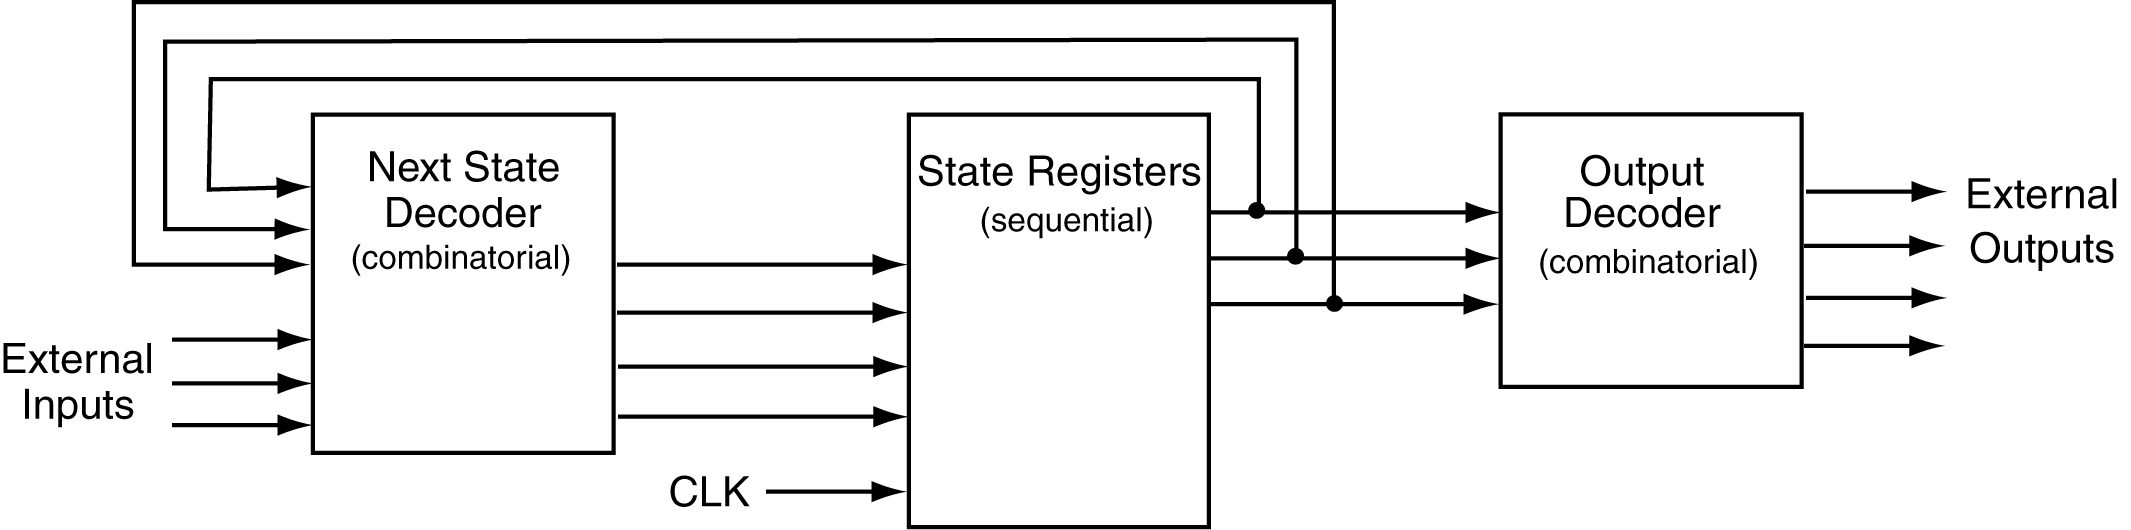
\includegraphics[width=13cm]{fsm/fsm.png}
	\caption{Block diagram for a Moore-type FSM.}
	\label{fsm}
\end{figure}

A block diagram for a standard Moore-type FSM is shown in Fig.~\ref{fsm}. This diagram looks fairly typical but different names are used for some of the blocks in the design. The \texttt{Next State Decoder} is a block of combinatorial logic that uses the current external inputs and the current state to decide upon the next state of the FSM. In other words, the inputs to the \texttt{Next State Decoder} block are decoded to produce an output that represents the next state of the FSM. The circuitry in \texttt{Next State Decoder} is generally the excitation equations for the storage elements (flip-flops) in the \texttt{State Register} block. The next state becomes the present state of the FSM when the clock input to the state registers block becomes active. The state registers block is a storage element that stores the present state of the machine. The inputs to the \texttt{Output Decoder} are used to generate the desired external outputs. The inputs are decoded via combinatorial logic to produce the external outputs. Because the external outputs are only dependent upon the current state of the machine, this FSM is classified as a Moore-type FSM.

The FSM model shown in Fig.~\ref{fsm} is probably the most common model for describing a Moore-type FSM. That is most likely because students are often asked to generate the combinatorial logic required to implement the \texttt{Next State Decoder} and the \texttt{Output Decoder}; however here we want to think about FSMs in the context of VHDL. The true power of VHDL starts to emerge in its dealings with FSMs. As you will see, the versatility of VHDL behavioral modeling removes the need for large paper designs of endless K-maps and endless combinatorial logic elements.

\begin{figure}[t]
    \centering
	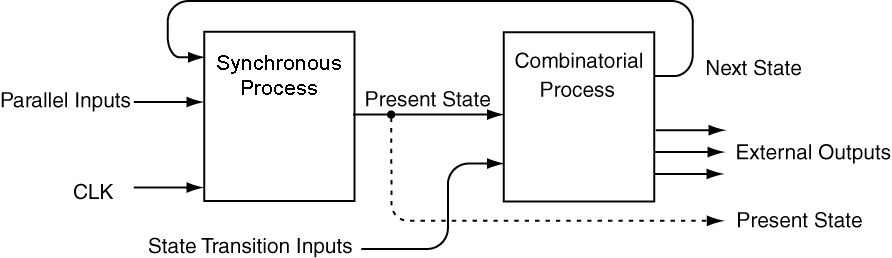
\includegraphics[width=12cm]{fsm/fsm_imp.png}
	\caption{Model for VHDL implementations of FSMs.}
	\label{fsm_imp}
\end{figure}

There are several different approaches used to model FSMs using VHDL. The many different possible approaches are a result of the general versatility of VHDL as a language. What we will describe in this section is probably the clearest approach for FSM implementation. A block diagram of the approach we will use in the implementation of FSMs is shown in Fig.~\ref{fsm_imp}.

Although it does not look that much clearer, you will soon be finding the FSM model shown in Fig.~\ref{fsm_imp} to be a straightforward method to implement FSMs. The approach we will use divides the FSM into two VHDL processes. One process, referred to as the \texttt{Synchronous Process} handles all the matters regarding clocking and other controls associated with the storage element. The other process, the \texttt{Combinatorial Process}, handles all the matters associated with the \texttt{Next State Decoder} and the \texttt{Output Decoder} of Fig.~\ref{fsm}. Note that the two blocks in Fig.~\ref{fsm} are both comprised solely of combinatorial logic.


There is some new lingo used in the description of signals used in Fig.~\ref{fsm_imp}; this description is outlined and described below: 
\begin{my_list}
\item The inputs labelled \texttt{Parallel Inputs} are used to signify inputs that act in parallel to each of the storage elements. These inputs would include enables, presets, clears, etc. 

\item The inputs labelled \texttt{State Transition Inputs} include external inputs that control the state transitions. These inputs also include external inputs used to decode Mealy-type external outputs. 

\item The \texttt{Present State} signals are used by the \texttt{Combinatorial Process} box for both next state decoding and output decoding. The diagram of Fig.~\ref{fsm_imp} also shows that the \texttt{Present State} variables can also be provided as outputs to the FSM but they are not required.
\end{my_list}

One final comment before we begin. Although there are many different methods that can be used to described FSMs using VHDL, two of the more common approaches are the dependent and independent PS/NS styles. This book only covers the dependent style because it is clearer than the independent PS/NS style. The model shown in Fig.~\ref{fsm_imp} is actually a model of the dependent PS/NS style of FSMs. Once you understand the VHDL modeling of the dependent PS/NS style of FSM, the understanding of the independent PS/NS style or any other style is relatively painless. More information on the other FSM coding styles is found in various VHDL texts or on the web.

\section{VHDL Behavioral Representation of FSMs}

\begin{leftbar}
\begin{minipage}[t]{0.5\textwidth}
\vspace{10pt}
\noindent
\textbf{EXAMPLE 18.}
Write the VHDL code that implements the FSM shown on the right. Use a dependent PS/NS coding style in your implementation.
\end{minipage}
\begin{minipage}[t]{0.47\textwidth}
\vspace{0pt}\raggedright
    \centering
	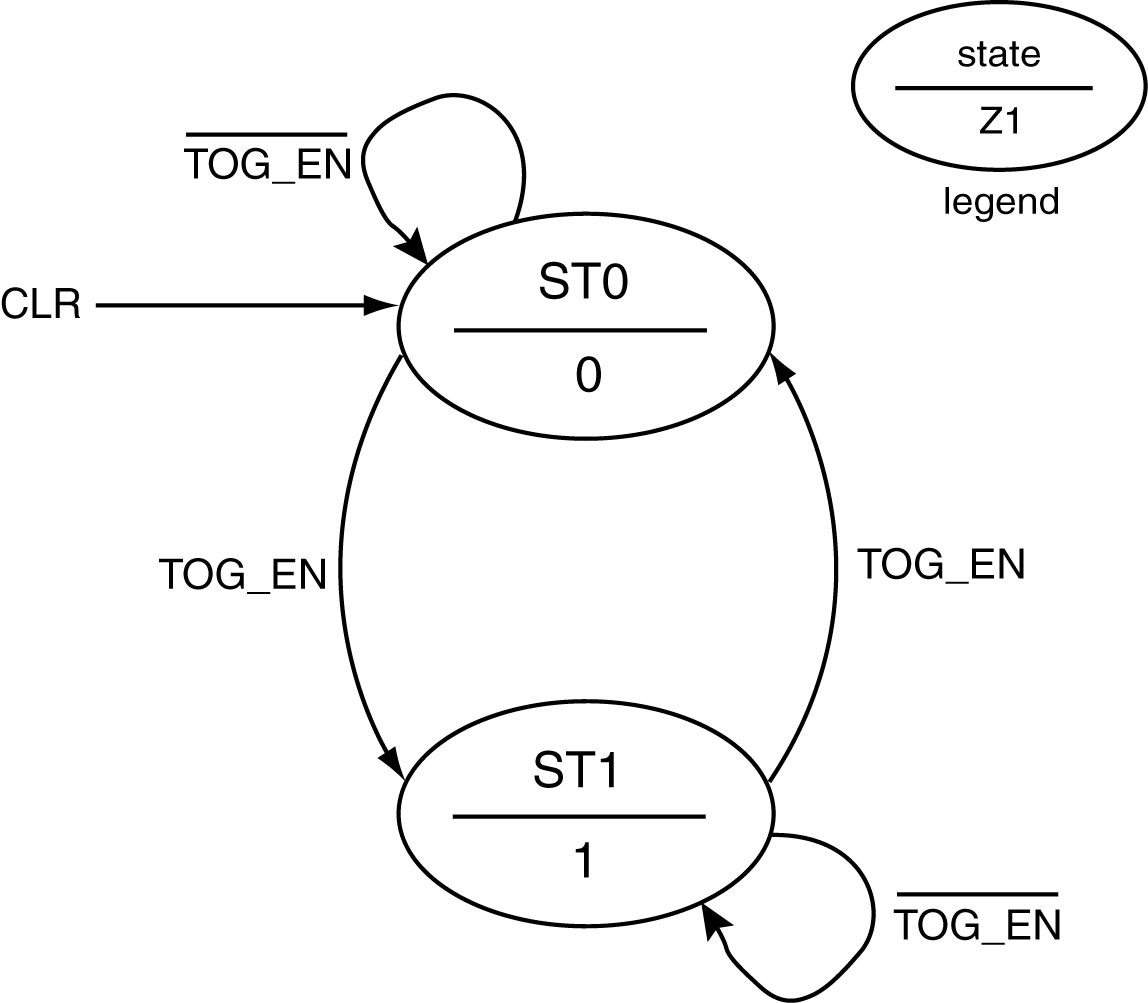
\includegraphics[width=5.3cm]{fsm/ex18.png}
\end{minipage}
\end{leftbar}
\noindent
\textbf{SOLUTION.} This problem represents a basic FSM implementation. It is somewhat instructive to show the black-box diagram which is an aid in writing the entity description. Starting FSM problems with the drawing of a black box diagram is always a healthy approach particularly when dealing with FSMs. Oftentimes with FSM problems, it becomes challenging to discern the FSM inputs from the outputs. Drawing a diagram partially alleviates this problem. The black box diagram and the code for the solution of Example 18 is shown in Listing \ref{exe_18_code}.

\begin{figure}[!h]
    \centering
	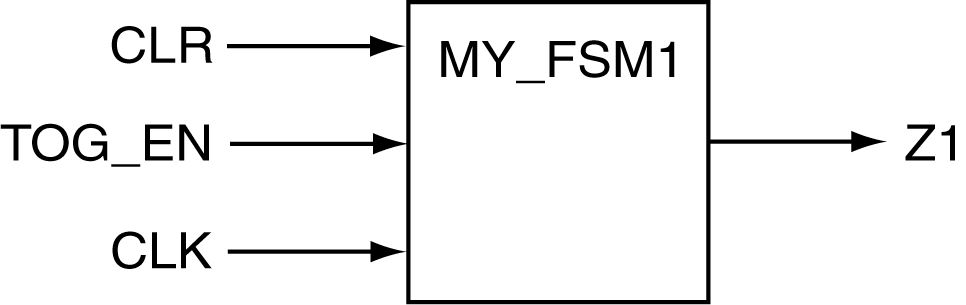
\includegraphics[width=5cm]{fsm/ex18_sol.png}
\end{figure}

\noindent
\begin{minipage}{0.99\linewidth}
\begin{lstlisting}[label=exe_18_code, caption=Solution to Example 18.]
-- library declaration
library IEEE;
use IEEE.std_logic_1164.all;
-- entity
entity my_fsm1 is 
    port (  TOG_EN  : in  std_logic; 
            CLK,CLR : in  std_logic; 
                 Z1 : out std_logic); 
end my_fsm1;
-- architecture
architecture fsm1 of my_fsm1 is
   type state_type is (ST0,ST1); 
   signal PS,NS : state_type; 
begin
   sync_proc: process(CLK,NS,CLR)
   begin
     -- take care of the asynchronous input
     if (CLR = '1') then 
        PS <= ST0;  
     elsif (rising_edge(CLK)) then 
        PS <= NS; 
     end if; 
   end process sync_proc; 

   comb_proc: process(PS,TOG_EN)
   begin
      Z1 <= '0';        -- pre-assign output
      case PS is 
         when ST0 =>    -- items regarding state ST0
            Z1 <= '0';  -- Moore output
            if (TOG_EN = '1') then NS <= ST1; 
            else  NS <= ST0; 
            end if; 
         when ST1 =>    -- items regarding state ST1
            Z1 <= '1';  -- Moore output
            if (TOG_EN = '1') then NS <= ST0; 
            else  NS <= ST1; 
            end if; 
         when others => -- the catch-all condition
            Z1 <= '0';  -- arbitrary; it should never 
            NS <= ST0;  -- make it to these two statements
      end case; 
   end process comb_proc; 
end fsm1;
\end{lstlisting}
\end{minipage}

And of course, this solution has many things worth noting in it. The more interesting things are listed below. 

\begin{my_list}
\item We have declared a special VHDL type named \texttt{state\_type} to represent the states in this FSM. This is an example of how enumeration types are used in VHDL. As with enumeration types in other higher-level computer languages, there are internal numerical representations for the listed state types but we only deal with the more expressive symbolic equivalent. In this case, the type we have created is called a \texttt{state\_type} and we have declared two variables of this type: PS and NS. The key thing to note here is that a \texttt{state\_type} is something we have created and is not a native VHDL type.

\item The synchronous process is equal in form and function to the simple D flip-flops we examined in the section about sequential circuits. The only difference is that we have substituted PS and NS for D and Q, respectively. Something to note here is that the storage element is associated with the PS signal only. Note that PS is not specified for every possible combination of inputs. 

\item Even though this example is of the simplest FSM you could hope for, the code looks somewhat complicated. But if you examine it closely, you can see that everything is nicely compartmentalized in the solution. There are two processes; the synchronous process handles the asynchronous reset and the assignment of a new state upon the arrival of the system clock. Additionally, the combinational process handles the outputs not handled in the synchronous process. 

\item Because the two processes operate concurrently, they can be considered as working in a lock-step manner. Changes to the NS signal that are generated in the combinatorial process force an evaluation of the synchronous process. When the changes are actually instituted in the synchronous process on the next clock edge, the changes in the PS signal causes the combinatorial process to be evaluated. And so on and so forth. 

\item The case statement in the combinatorial process provides a \texttt{when} clause for each state of the FSM. This is the standard approach for the dependent PS/NS coding style. A \texttt{when others} clause has also been used. The signal assignments that are part this catch-all clause are arbitrary since the code should never actually make it there. This statement is provided for a sense of completeness and represents good VHDL coding practice. 

\item The Moore output is a function of only the present state. This is expressed by the fact that the assignment of the Z1 output is unconditionally evaluated in each when clause of the case statement in the combinatorial process. In other words, the Z1 variable is inside the \texttt{when} clause but outside of the \texttt{if} statement in the \texttt{when} clause. This is of course because the Moore outputs are only a function of the states and not the external inputs. Note that it is the external input that controls the \texttt{which} state the FSM transitions to from any given state. You will see later that Mealy outputs, due their general nature, are assigned inside the \texttt{if} statement.

\item The Z1 output is pre-assigned as the first step in the combinatorial process. Pre-assigning it in this fashion prevents the unexpected latch generation for the Z1 signal. When dealing with FSMs, there is a natural tendency for the FSM designer to forget to specify an output for the Z1 variable in each of the states. Pre-assigning it prevents latches from being generated and can arguably clean up the source code. The pre-assignment makes no difference to the VHDL code because if multiple assignments are made within the code, only the final assignment takes effect. In other words, only the final assignment is considered once the process terminates. 
\end{my_list}

There is one final thing to note about Example 18. In an effort to keep the example simple, we disregarded the digital values of the state variables. This is indicated in the black-box diagram of Listing \ref{exe_18_code} by the fact that the only output of the FSM is the signal Z1. This is reasonable in that it could be considered that only one output was required in order to control some other device or circuit. The state variable is represented internally and its precise representation is not important since the state variable is not provided as an output. 

In some FSM designs, the state variables are provided as outputs. To show this situation, we will provide a solution to Example 18 with the state variables as outputs. The black-box diagram and the VHDL code of this solution is shown in Listing \ref{exe_18_code_alt}.
\begin{figure}[!h]
    \centering
	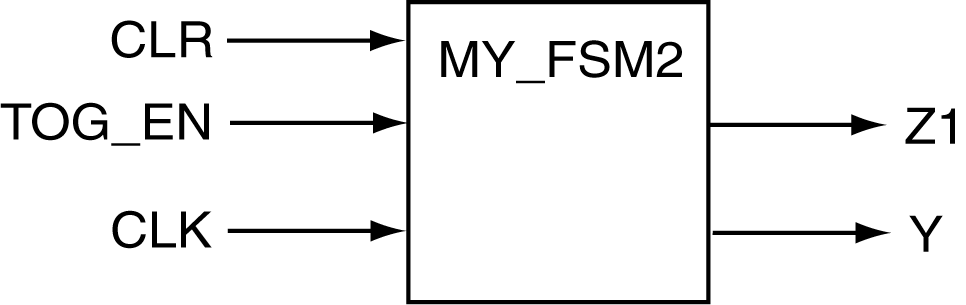
\includegraphics[width=5cm]{fsm/ex18_sol_alt.png}
\end{figure}

\noindent
\begin{minipage}{0.99\linewidth}
\begin{lstlisting}[label=exe_18_code_alt, caption=Solution to Example 18 that include state variable as output.]
-- library declaration
library IEEE;
use IEEE.std_logic_1164.all;
-- entity
entity my_fsm2 is 
   port (   TOG_EN : in  std_logic; 
           CLK,CLR : in  std_logic; 
              Y,Z1 : out std_logic); 
end my_fsm2;
-- architecture
architecture fsm2 of my_fsm2 is
   type state_type is (ST0,ST1); 
   signal PS,NS : state_type; 
begin
   sync_proc: process(CLK,NS,CLR)
   begin
      if (CLR = '1') then 
         PS <= ST0; 
      elsif (rising_edge(CLK)) then 
         PS <= NS; 
      end if; 
   end process sync_proc; 

   comb_proc: process(PS,TOG_EN)
   begin
      Z1 <= '0';
      case PS is    
         when ST0 =>        -- items regarding state ST0
            Z1 <= '0';      -- Moore output
            if (TOG_EN = '1') then NS <= ST1; 
            else  NS <= ST0; 
            end if; 
         when ST1 =>        -- items regarding state ST1
            Z1 <= '1';      -- Moore output
            if (TOG_EN = '1') then NS <= ST0; 
            else  NS <= ST1; 
            end if; 
         when others =>     -- the catch-all condition
            Z1 <= '0';      -- arbitrary; it should never 
            NS <= ST0;      -- make it to these two statements
      end case; 
   end process comb_proc; 
 
   -- assign values representing the state variables
   with PS select
      Y <= '0' when ST0, 
           '1' when ST1, 
           '0' when others; 
end fsm2;
\end{lstlisting}
\end{minipage}

Note that the VHDL code shown in Listing \ref{exe_18_code_alt} differs in only two areas from the code shown in Listing \ref{exe_18_code}. The first area is the modification of the entity declaration to account for the state variable output Y. The second area is the inclusion of the selective signal assignment statement which assigns a value of state variable output Y based on the condition of the state variable. The selective signal assignment statement is evaluated each time a change in signal PS is detected. Once again, since we have declared an enumeration type for the state variables, we have no way of knowing exactly how the synthesizer will decide to represent the state variable. The selective signal assignment statement in the code of Listing \ref{exe_18_code_alt} only makes it appear like there is one state variable and the states are represented with a '1' and a '0'. In reality, there are methods we can use to control how the state variables are represented and we will deal with those soon. 

Lastly, there are three concurrent statements in the VHDL code shown in Listing \ref{exe_18_code_alt}: two process statements and a selective signal assignment statement. 

\begin{leftbar}
\begin{minipage}[t]{0.5\textwidth}
\vspace{10pt}
\noindent
\textbf{EXAMPLE 19.}
Write the VHDL code that implements the FSM shown on the right. Use a dependent PS/NS coding style in your implementation. Consider the state variables as outputs of the FSM.
\end{minipage}
\begin{minipage}[t]{0.47\textwidth}
\vspace{0pt}\raggedright
\centering
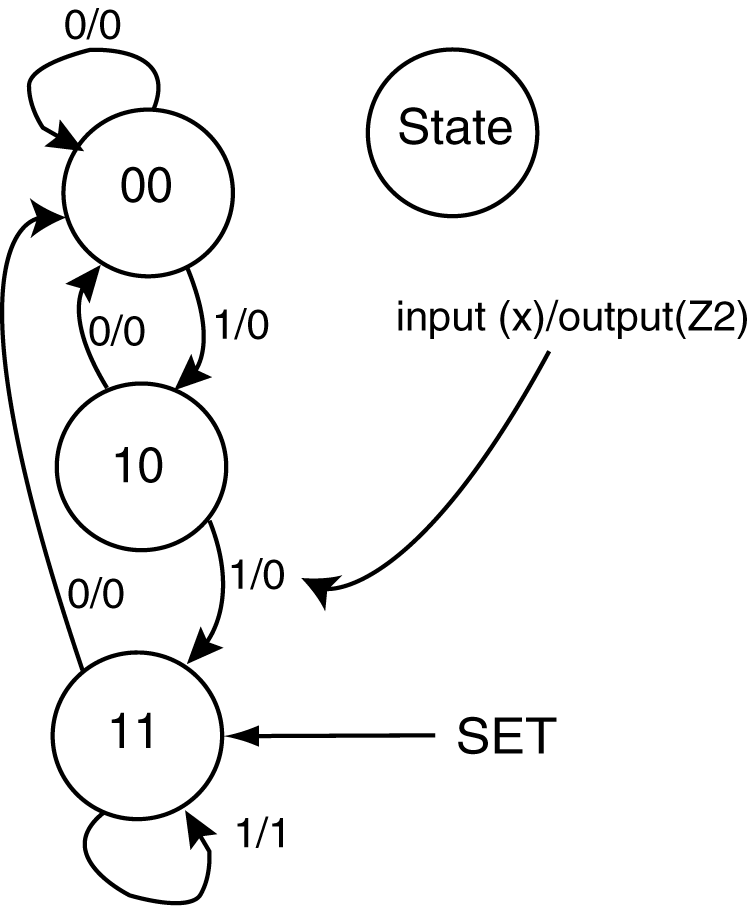
\includegraphics[width=5cm]{fsm/ex19.png}
\end{minipage}
\end{leftbar}
\noindent
\textbf{SOLUTION.} The state diagram shown in this problem indicates that this is a three-state FSM with one Mealy-type external output and one external input. Since there are three states, the solution requires at least two state variables to handle the three states. The black-box diagram of the solution is shown in Listing \ref{exe_19_code}. Note that the two state variables are handled as a bundled signal.


\begin{figure}[!h]
    \centering
	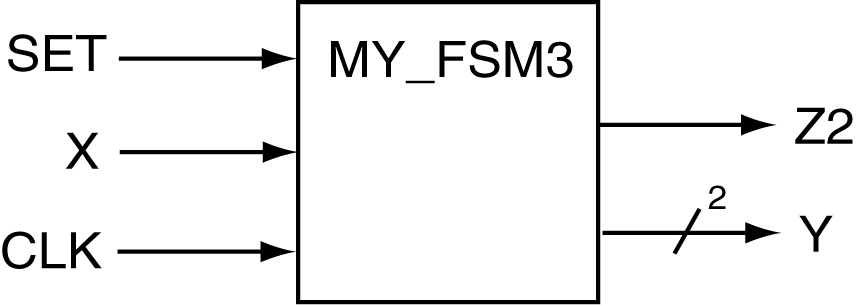
\includegraphics[width=5cm]{fsm/ex19_sol.png}
\end{figure}

\noindent
\begin{minipage}{0.99\linewidth}
\begin{lstlisting}[label=exe_19_code, caption=Solution to Example 19.]
-- library declaration
library IEEE;
use IEEE.std_logic_1164.all;
-- entity
entity my_fsm3 is 
    port ( X,CLK,SET : in  std_logic; 
                   Y : out std_logic_vector(1 downto 0); 
                  Z2 : out std_logic); 
end my_fsm3;
-- architecture
architecture fsm3 of my_fsm3 is
   type state_type is (ST0,ST1,ST2); 
   signal PS,NS : state_type; 
begin
   sync_proc: process(CLK,NS,SET)
   begin
      if (SET = '1') then 
         PS <= ST2; 
      elsif (rising_edge(CLK)) then 
         PS <= NS; 
      end if; 
   end process sync_proc; 

   comb_proc: process(PS,X)
   begin
      Z2 <= '0';           -- pre-assign FSM outputs
      case PS is 
         when ST0 =>       -- items regarding state ST0
            Z2 <= '0';     -- Mealy output always 0
            if (X = '0') then NS <= ST0;  
            else  NS <= ST1; 
            end if; 
         when ST1 =>       -- items regarding state ST1
            Z2 <= '0';     -- Mealy output always 0
            if (X = '0') then NS <= ST0; 
            else  NS <= ST2; 
            end if; 
         when ST2 =>       -- items regarding state ST2
            -- Mealy output handled in the if statement
            if (X = '0') then NS <= ST0; Z2 <= '0'; 
            else  NS <= ST2;  Z2 <= '1';     
            end if; 
         when others =>    -- the catch all condition
            Z2 <= '1'; NS <= ST0; 
      end case; 
   end process comb_proc; 
 
   -- faking some state variable outputs
   with PS select
      Y <= "00" when ST0, 
           "10" when ST1, 
           "11" when ST2, 
           "00" when others; 
end fsm3;
\end{lstlisting}
\end{minipage}

As usual, there are a couple of fun things to point out about the solution for Example 19. Most importantly, you should note the similarities between this solution and the previous solution. 

\begin{my_list}
\item The FSM has one Mealy-type output. The solution essentially treats this output as a Moore-type output in the first two \texttt{when} clauses of the \texttt{case} statement. In the final \texttt{when} clause, the Z2 output appears in both sections of the \texttt{if} statement. The fact the Z2 output is different in the context of state ST2 that makes it a Mealy-type output and therefore a Mealy-type FSM. 

\item When faking the state variable outputs (keeping in mind that the actual state variables are represented with enumeration types), two signals are required since the state diagram contains more than two states (and less than five states). The solution opted is to represent these outputs as a bundle which has the effect of slightly changing the form of the selected signal assignment statement appearing at the end of the architecture description. 
\end{my_list}

\begin{leftbar}
\begin{minipage}[t]{0.5\textwidth}
\vspace{10pt}
\noindent
\textbf{EXAMPLE 20.}
Write the VHDL code that implements the FSM shown on the right. Use a dependent PS/NS coding style in your implementation. Consider the listed state variables as output.
\end{minipage}
\begin{minipage}[t]{0.47\textwidth}
\vspace{0pt}\raggedright
\centering
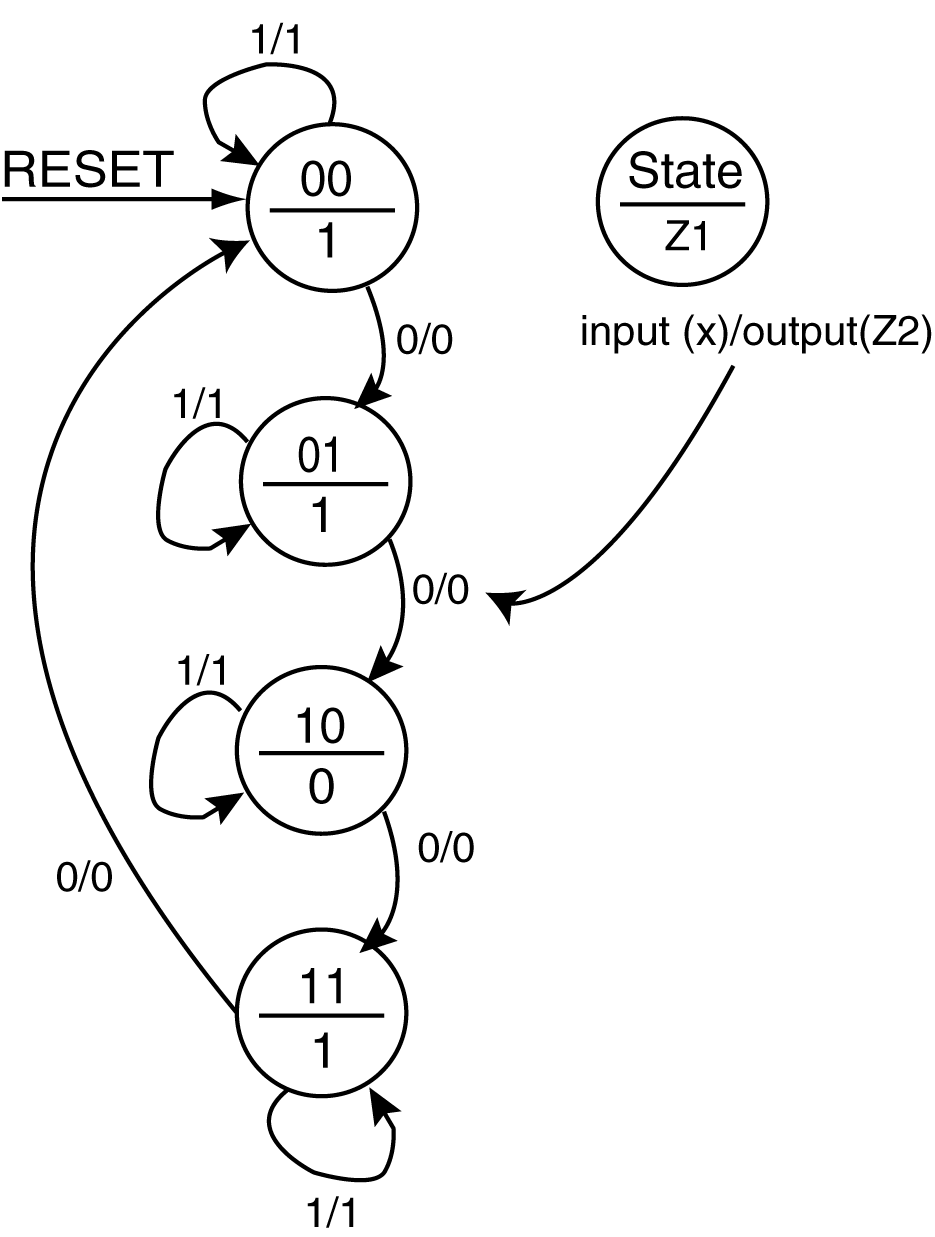
\includegraphics[width=5.2cm]{fsm/ex20.png}
\end{minipage}
\end{leftbar}

\noindent
\textbf{SOLUTION.} The state diagram indicates that its implementation will contain four states, one external input and two external outputs. This is a hybrid FSM in that the if contains both a Mealy and Moore-type output but in this case, the FSM would be considered a Mealy-type FSM. The black-box diagram and the actual solution for the solution is shown in Listing \ref{exe_20_code}. 
\begin{figure}[!h]
    \centering
	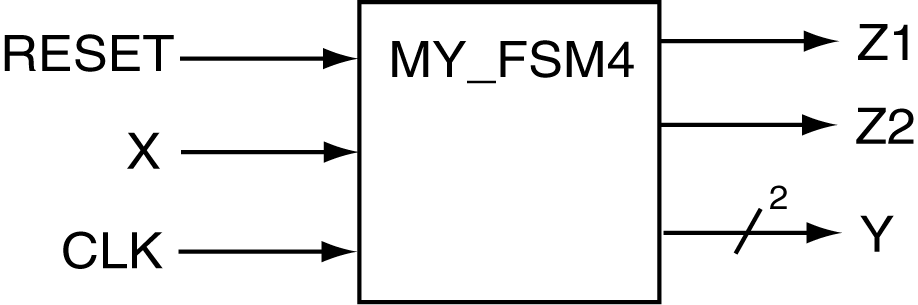
\includegraphics[width=5cm]{fsm/ex20_sol.png}
\end{figure}

\noindent
\begin{minipage}{0.99\linewidth}
\begin{lstlisting}[label=exe_20_code, caption=Solution to Example 20.]
-- library declaration
library IEEE;
use IEEE.std_logic_1164.all;
-- entity
entity my_fsm4 is 
    port ( X,CLK,RESET : in  std_logic; 
                     Y : out std_logic_vector(1 downto 0); 
                 Z1,Z2 : out std_logic);  
end my_fsm4;
-- architecture
architecture fsm4 of my_fsm4 is
   type state_type is (ST0,ST1,ST2,ST3); 
   signal PS,NS : state_type; 
begin
   sync_proc: process(CLK,NS,RESET)
   begin
     if (RESET = '1') then  PS <= ST0; 
     elsif (rising_edge(CLK)) then  PS <= NS; 
     end if; 
   end process sync_proc; 

   comb_proc: process(PS,X)
   begin
      -- Z1: the Moore output; Z2: the Mealy output
      Z1 <= '0';   Z2 <= '0'; -- pre-assign the outputs
      case PS is 
         when ST0 =>    -- items regarding state ST0
            Z1 <= '1';  -- Moore output 
            if (X = '0') then NS <= ST1; Z2 <= '0';   
            else  NS <= ST0; Z2 <= '1';
            end if; 
         when ST1 =>    -- items regarding state ST1
            Z1 <= '1';  -- Moore output 
            if (X = '0') then NS <= ST2; Z2 <= '0';  
            else  NS <= ST1; Z2 <= '1'; 
            end if; 
         when ST2 =>    -- items regarding state ST2
            Z1 <= '0';  -- Moore output 
            if (X = '0') then NS <= ST3; Z2 <= '0'; 
            else  NS <= ST2; Z2 <= '1'; 
            end if; 
         when ST3 =>    -- items regarding state ST3
            Z1 <= '1';  -- Moore output 
            if (X = '0') then NS <= ST0; Z2 <= '0'; 
            else  NS <= ST3;  Z2 <= '1';     
            end if; 
         when others => -- the catch all condition
            Z1 <= '1';  Z2 <= '0';  NS <= ST0; 
      end case; 
   end process comb_proc; 
 
   with PS select
      Y <= "00" when ST0, 
           "01" when ST1, 
           "10" when ST2, 
           "11" when ST3, 
           "00" when others; 
end fsm4;
\end{lstlisting}
\end{minipage}

If you haven't noticed by now, implementing FSMs using the VHDL behavioral model is remarkably straightforward. In reality, I rarely code a FSM from scratch; I usually opt to grab some previous FSM I have coded and start from there. Keep in mind that real engineering is rarely based on a cookbook. For FSM problems, the engineering is in the testing and creation of the state diagram. Do not get too comfortable with behavioral modeling of FSMs; the real fun is actually generating a FSM that solves a given problem. 

\section{One-Hot Encoding for FSMs}
Truth told, there are many different methods that can be used to encode state variables\footnote{In this case, encoding refers to the act of assigning a unique pattern of  1's and 0's to each of the state in order to make them unambiguous from other states.}. If the exact form of the representation used is important to you, then you will need to take the necessary steps in order to control how the state variables are represented by the synthesizer. There are two approaches to control state variable representation. The first approach is to allow the synthesizing tool to handle the details. Since every FSM we have seen up to this point has used enumeration types to represent the state variables, the synthesizer could choose to actually represent them with an encoding scheme of its own choosing. The reality is that the tools generally have an option to select the desired encoding scheme. The downside of this approach is that you are denied the learning experience associated with implementing the VHDL code that explicitly induces your desired encoding scheme. After all, you may have some special encoding scheme you need to use but is not supported by the development tools. The second approach to encoding the state variables is to specify them directly in VHDL. The approach of specifying the state variables in the VHDL code is presented in this section. 

One-hot encoding uses one bit in the state register for each state of the FSM. For a one-hot encoding FSM with 16 states, 16 flip flops are required. However only four flip flops are required if the same FSM is implemented using a binary encoding. One-hot encoding simplifies the logic and the interconnections between overall logic. Despite looking quite wasteful in terms of employed logic, one-hot encoding often results in smaller and faster FSMs.

The approach taken in the previous FSM examples was to pretend we were using full encoding for the state variables of the FSM. The full encoding approach minimizes the number of storage elements (flip-flops) used to store the state variables. The closed form equation describing the number of flip-flops required for a given FSM as a function of the number of states is shown in equation \ref{eq1}. The bracket-like symbols used in equation \ref{eq1} indicate a ceiling function\footnote{The ceiling function $y=\lceil x \rceil$ assigns $y$ to the smallest integer that is greater or equal to $x$.}. The binary nature expressed by this equation is so apparent that this encoding is often referred to as binary encoding.

\begin{equation}\label{eq1}
 \#(flip\_flops) = \lceil \log_2(\#states) \rceil
\end{equation}

For one-hot encoded FSMs, only one flip-flop is asserted at any given time. This requires that each distinct state be represented by one flip-flop. In one-hot encoding, the number of flip-flops required to implement a FSM is therefore equal to the number of states in the FSM. The closed form of this relationship is shown in equation \ref{eq2}. 

\begin{equation}\label{eq2}
 \#(flip\_flops) = \lceil \#(states) \rceil
\end{equation}

The question naturally arises as to how VHDL can be used to implement one-hot encoded FSMs. If you want total control of the process, you will need to grab control away from the synthesizer. And since we are concerned with learning VHDL, we need to look at the process of explicitly encoding one-hot FSMs. 

The modular approach we used to implement FSMs expedites the conversion process from using enumeration types to actually specifying how the state variables are represented. The changes from our previous approach are limited to how the outputs are assigned to the state variables and how the state variables are forced to be represented by certain bit patterns. Modifications to the full encoded approach are thus limited to the entity declaration (you will need more variables to represent the states), the declaration of the state variables (you will need to explicitly declare the bit patterns associated with each state) and the assignment of the state variables to the outputs (in this case, we are actually not faking it like we were in other examples). 

\begin{leftbar}
\begin{minipage}[t]{0.5\textwidth}
\vspace{10pt}
\noindent
\textbf{EXAMPLE 21.}
Write the VHDL code that implements the FSM shown on the right. Use a dependent PS/NS coding style in your implementation. Consider the listed state variables as output. Use one-hot encoding for the state variables. This problem is Example 20 all over again but uses true one-hot encoding for the state variables. 
\vspace{50px}
\end{minipage}
\begin{minipage}[t]{0.47\textwidth}
\vspace{0pt}\raggedright
    \centering
	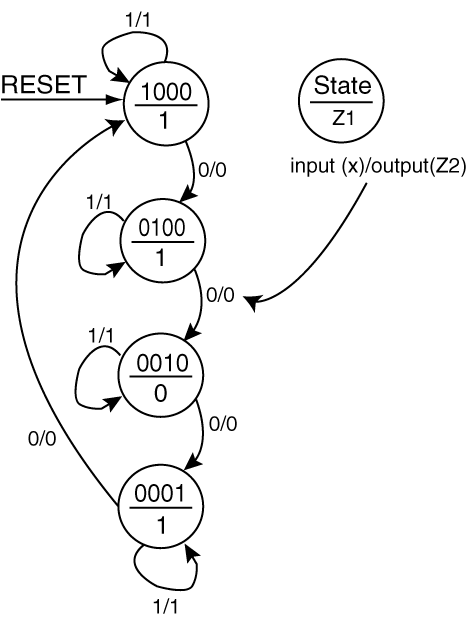
\includegraphics[width=5cm]{fsm/ex21.png}
\end{minipage}
\end{leftbar}
\noindent
\textbf{SOLUTION.} The state diagram shows four states, one external input X, two external outputs Z1 and Z2 with the Z2 output being a Mealy output. This is a Mealy machine that indicates one-hot encoding should be used to encode the state variables. We will approach the implementation of this FSM one piece at the time.

Listing \ref{exe_21_code_1} shows the modifications to the entity declaration required to convert the full encoding used in Example 20 to a pseudo one-hot encoding. Listing \ref{exe_21_code_2} shows the required modifications to the state variable output assignment in order to move from enumeration types to a special form of assigned types. Forcing the state variables to be truly encoded using one-hot encoding requires these two extra lines of code as is shown in Listing \ref{exe_21_code_2}. These two lines of code essentially force the VHDL synthesizer to represent each state of the FSM with its own storage element. In other words, each state is represented by the "string" modifier as listed. This forces four bits per state to be remembered by the FSM implementation which essentially requires four flip-flops. Note in Listing \ref{exe_21_code_3} that the default case is assigned a valid one-hot state instead of the customary all zero state. You should strongly consider comparing these three figures. The total solution is shown in Listing \ref{exe_21_code_4} 

\noindent
\begin{minipage}{0.99\linewidth}
\begin{lstlisting}[label=exe_21_code_1, caption=Modifications to convert Example 20 to one-hot encoding.]
-- full encoded approach
entity my_fsm4 is 
    port ( X,CLK,RESET : in  std_logic; 
                     Y : out std_logic_vector(1 downto 0); 
                 Z1,Z2 : out std_logic);  
end my_fsm4;
----------------------------------------------------------------------
-- one-hot encoding approach
entity my_fsm4 is 
    port ( X,CLK,RESET : in  std_logic; 
                     Y : out std_logic_vector(3 downto 0); 
                 Z1,Z2 : out std_logic);  
end my_fsm4;
\end{lstlisting}

\begin{lstlisting}[label=exe_21_code_2, caption=Modifications to convert state variables to use one-hot encoding.]
-- the approach for enumeration types   
type state_type is (ST0,ST1,ST2,ST3); 
signal PS,NS : state_type; 
----------------------------------------------------------------------
-- the approach used for explicitly specifying state bit patterns
type state_type is (ST0,ST1,ST2,ST3); 
attribute ENUM_ENCODING: STRING; 
attribute ENUM_ENCODING of state_type: type is "1000 0100 0010 0001";
signal PS,NS : state_type;
\end{lstlisting}
\end{minipage}

\noindent
\begin{minipage}{0.99\linewidth}
\begin{lstlisting}[label=exe_21_code_3, caption=Modifications to convert state output to pseudo one-hot encoding.]
-- fake full encoded approach 
with PS select
   Y <= "00" when ST0, 
        "01" when ST1, 
        "10" when ST2, 
        "11" when ST3, 
        "00" when others; 
end fsm4;
----------------------------------------------------------------------
-- one-hot encoded approach 
with PS select
   Y <= "1000" when ST0, 
        "0100" when ST1, 
        "0010" when ST2, 
        "0001" when ST3, 
        "1000" when others; 
end fsm4;
\end{lstlisting}
\end{minipage}

\noindent
\begin{minipage}{0.99\linewidth}
\begin{lstlisting}[label=exe_21_code_4, caption=The final solution to Example 21.]
-- library declaration
library IEEE;
use IEEE.std_logic_1164.all;
-- entity
entity my_fsm4_oh is 
    port ( X,CLK,RESET : in  std_logic; 
                     Y : out std_logic_vector(3 downto 0); 
                 Z1,Z2 : out std_logic);  
end my_fsm4_oh;
-- architeture
architecture fsm4_oh of my_fsm4_oh is
  type state_type is (ST0,ST1,ST2,ST3);
  attribute ENUM_ENCODING: STRING; 
  attribute ENUM_ENCODING of state_type: type is "1000 0100 0010 0001";
  signal PS,NS : state_type; 
begin
   sync_proc: process(CLK,NS,RESET)
   begin
     if (RESET = '1') then  PS <= ST0; 
     elsif (rising_edge(CLK)) then  PS <= NS; 
     end if; 
   end process sync_proc; 

   comb_proc: process(PS,X)
   begin
      -- Z1: the Moore output; Z2: the Mealy output
      Z1 <= '0';   Z2 <= '0'; -- pre-assign the outputs
      case PS is 
         when ST0 =>    -- items regarding state ST0
            Z1 <= '1';  -- Moore output 
            if (X = '0') then NS <= ST1; Z2 <= '0';   
            else  NS <= ST0; Z2 <= '1';
            end if; 
         when ST1 =>    -- items regarding state ST1
            Z1 <= '1';  -- Moore output 
            if (X = '0') then NS <= ST2; Z2 <= '0';  
            else  NS <= ST1; Z2 <= '1'; 
            end if; 
         when ST2 =>    -- items regarding state ST2
            Z1 <= '0';  -- Moore output 
            if (X = '0') then NS <= ST3; Z2 <= '0'; 
            else  NS <= ST2; Z2 <= '1'; 
            end if; 
         when ST3 =>    -- items regarding state ST3
            Z1 <= '1';  -- Moore output 
            if (X = '0') then NS <= ST0; Z2 <= '0'; 
            else  NS <= ST3;  Z2 <= '1';     
            end if; 
         when others => -- the catch all condition
            Z1 <= '1';  Z2 <= '0';  NS <= ST0; 
      end case; 
   end process comb_proc; 
 
   -- one-hot encoded approach 
   with PS select
      Y <= "1000" when ST0, 
           "0100" when ST1, 
           "0010" when ST2, 
           "0001" when ST3, 
           "1000" when others; 

end fsm4_oh;
\end{lstlisting}
\end{minipage}

\section{Important Points}

\begin{my_list}
\item Modeling FSMs from a state diagram is a straightforward process using VHDL behavioral modeling. The process is so straightforward that it is often considered cookie cutter. The real engineering involved in implementing FSM is in the generation of the state diagram that solved the problem at hand.

\item Due to the general versatility of VHDL, there are many approaches that can be used to model FSMs using VHDL. The approach used here details only one of those styles but is generally considered the most straightforward of all styles. 

\item The actual encoding of the FSM's state variables when enumeration types are used is left up to the synthesis tool. If a preferred method of variable encoding is desired, using the attribute approach detail in this section is a simple but viable alternative. 
\end{my_list}

\section{Exercises: Behavioral Modeling of FSMs}

%%%%%% EXERCISE 1 %%%%%%
\vspace{20pt}
\noindent
\begin{minipage}{1\textwidth}
\textbf{EXERCISE 1.}
Draw the state diagram associated with the following VHDL code. Be sure to provide a legend and completely label everything.
\end{minipage}
\begin{minipage}{0.66\textwidth}
\vspace{10px}
\begin{lstlisting}
-- library declaration
library IEEE;
use IEEE.std_logic_1164.all;
-- entity
entity fsm is 
   port (  X,CLK : in  std_logic; 
           RESET : in  std_logic; 
           Z1,Z2 : out std_logic;  
end fsm;
-- architecture
architecture fsm of fsm is
   type state_type is (A,B,C);
   signal PS,NS : state_type;
begin
   sync_proc: process(CLK,NS,RESET)
   begin
      if (RESET = '0') then PS <= C; 
      elsif (rising_edge(CLK)) then PS <= NS; 
      end if; 
   end process sync_proc; 

   comb_proc: process(PS,X)
   begin
      case PS is 
         Z1 <= '0';    Z2 <= '0'; 
         when A =>    
            Z1 <= '0';  
            if (X='0') then NS<=A; Z2<='1';   
            else  NS <= B; Z2 <= '0';
            end if; 
         when B =>    
            Z1 <= '1';  
            if (X='0') then NS<=A; Z2<='0';  
            else  NS <= C; Z2 <= '1'; 
            end if; 
         when C =>    
            Z1 <= '1';  
            if (X='0') then NS<=B; Z2<='1'; 
            else  NS <= A; Z2 <= '0'; 
            end if; 
         when others =>    
            Z1 <= '1'; NS<=A; Z2<='0'; 
      end case; 
   end process comb_proc; 
end fsm;
\end{lstlisting}
\end{minipage}
\begin{minipage}{0.29\textwidth}
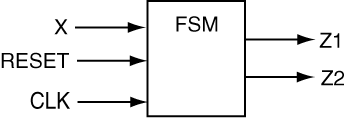
\includegraphics[width=4cm]{fsm/sm_ex1.png}
\vspace{250px}
\end{minipage}

%%%%%% EXERCISE 2 %%%%%%
\vspace{20pt}
\noindent
\begin{minipage}[t]{0.5\textwidth}
\textbf{EXERCISE 2.}
Write a VHDL behavioral model that could be used to implement the state diagram as shown on the right. The state variables should be encoded as listed and also provided as outputs of the FSM.
\end{minipage}
\begin{minipage}[t]{0.47\textwidth}
\vspace{0pt}\raggedright
\centering
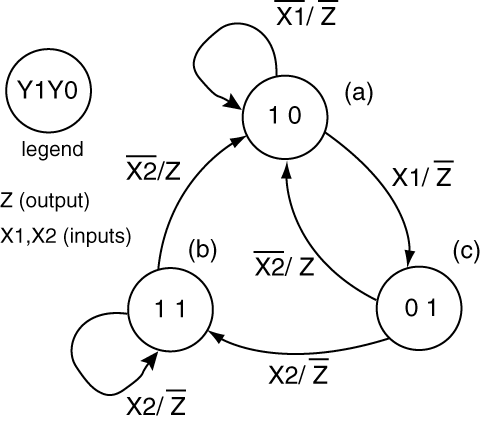
\includegraphics[width=5.3cm]{fsm/sm_ex2.png}
\end{minipage}

%%%%%% EXERCISE 3 %%%%%%
\vspace{20pt}
\noindent
\begin{minipage}{1\textwidth}
\textbf{EXERCISE 3.}
Draw the state diagram associated with the following VHDL code. Be sure to provide a legend and remember to label everything.
\end{minipage}
\begin{minipage}{0.66\textwidth}
\vspace{10px}
\begin{lstlisting}
-- library declaration
library IEEE;
use IEEE.std_logic_1164.all;
-- entity
entity fsmx is
    Port ( BUM1,BUM2 : in  std_logic;
                 CLK : in   std_logic;
            TOUT,CTA : out std_logic);
end fsmx;
-- architecture
architecture my_fsmx of fsmx is
   type state_type is (S1,S2,S3); 
	signal PS,NS : state_type; 
begin
   sync_p: process (CLK,NS)
   begin
      if (rising_edge(CLK)) then   
         PS <= NS; 
      end if; 
   end process sync_p; 

   comb_p: process (CLK,BUM1,BUM2)
   begin
      case PS is 

         when S1 => 
            CTA <= '0'; 
            if (BUM1 = '0')  then 
               TOUT <= '0'; 
               NS <= S1; 
            elsif (BUM1 = '1') then 
               TOUT <= '1';  
               NS <= S2; 
            end if; 

         when S2 =>
            CTA <= '0'; 
            TOUT <= '0'; 
            NS <= S3;   

         when S3 =>
            CTA <= '1'; 
            TOUT <= '0';   
            if (BUM2 = '1')  then 
               NS <= S1; 
            elsif (BUM2 = '0') then 
               NS <= S2; 
            end if; 
      
         when others =>   CTA <= '0'; 
                         TOUT <= '0';
                           NS <= S1;
      end case; 
   end process comb_p; 
end my_fsmx;
\end{lstlisting}
\end{minipage}
\begin{minipage}{0.29\textwidth}
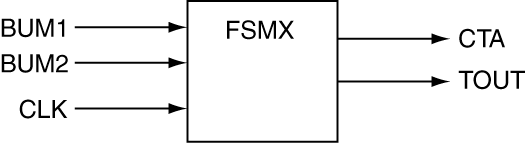
\includegraphics[width=4cm]{fsm/sm_ex3.png}
\vspace{250px}
\end{minipage}

%%%%%% EXERCISE 4 %%%%%%
\vspace{20pt}
\noindent
\begin{minipage}[t]{0.5\textwidth}
\textbf{EXERCISE 4.}
Write the VHDL behavioral model code that could be used to implement the state diagram on shown in the right.
\end{minipage}
\begin{minipage}[t]{0.47\textwidth}
\vspace{0pt}\raggedright
\centering
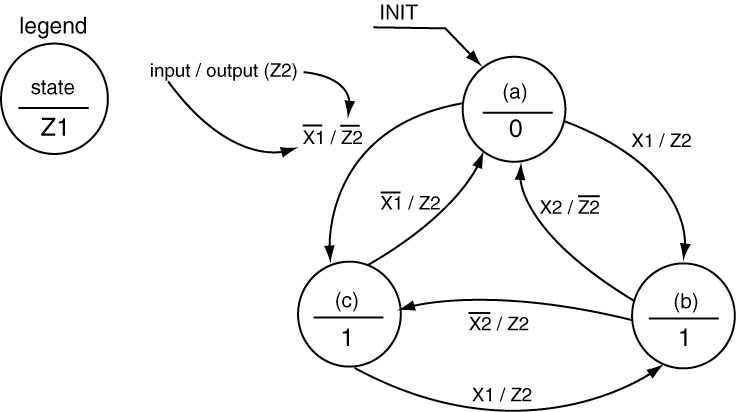
\includegraphics[width=5.7cm]{fsm/sm_ex4.png}
\end{minipage}

%%%%%% EXERCISE 5 %%%%%%
\vspace{20pt}
\noindent
\begin{minipage}{1\textwidth}
\textbf{EXERCISE 5.}
Draw the state diagram associated with the following VHDL code. Consider the outputs \texttt{Y} to be representative of the state variables. Be sure to provide a legend. Indicate the states with both state variables and their symbolic equivalents.
\end{minipage}
\begin{minipage}{1\textwidth}
\vspace{10px}
\begin{lstlisting}
-- library declaration
library IEEE;
use IEEE.std_logic_1164.all;
-- entity
entity fsm is 
port (     X,CLK : in  std_logic; 
           RESET : in  std_logic; 
           Z1,Z2 : out std_logic;  
               Y : out std_logic_vector(2 downto 0)); 
end fsm;
-- architecture
architecture my_fsm of fsm is
   type state_type is (A,B,C);
   attribute ENUM_ENCODING: STRING; 
   attribute ENUM_ENCODING of state_type: type is "001 010 100";
   signal PS,NS : state_type;
begin

sync_proc: process(CLK,NS,RESET) -- process
   begin
     if (RESET = '0') then PS <= C; 
     elsif (rising_edge(CLK)) then PS <= NS; 
     end if; 
   end process sync_proc; 

comb_proc: process(PS,X) -- process
   begin
      case PS is 
         when A =>    
            Z1 <= '0';  
            if (X = '0') then NS <= A; Z2 <= '1';   
            else  NS <= B; Z2 <= '0';
            end if; 
         when B =>    
            Z1 <= '1';  
            if (X = '0') then NS <= A; Z2 <= '0';  
            else  NS <= C; Z2 <= '1'; 
            end if; 
         when C =>    
            Z1 <= '1';  
            if (X = '0') then NS <= B; Z2 <= '1'; 
            else  NS <= A; Z2 <= '0'; 
            end if; 
         when others =>    
            Z1 <= '1'; NS <= A; Z2 <= '0';  
      end case; 
   end process comb_proc; 
 
with PS select
   Y <= "001" when A, 
        "010" when B, 
        "100" when C, 
        "001" when others; 
end my_fsm;
\end{lstlisting}
\end{minipage}

%%%%%% EXERCISE 6 %%%%%%
\vspace{20pt}
\noindent
\begin{minipage}[t]{0.5\textwidth}
\textbf{EXERCISE 6.}
Write a VHDL behavioral model code that can be used to implement the state diagram shown on the right. All state variables should be encoded as listed and also provided as outputs of the FSM.
\end{minipage}
\begin{minipage}[t]{0.47\textwidth}
\vspace{0pt}\raggedright
\centering
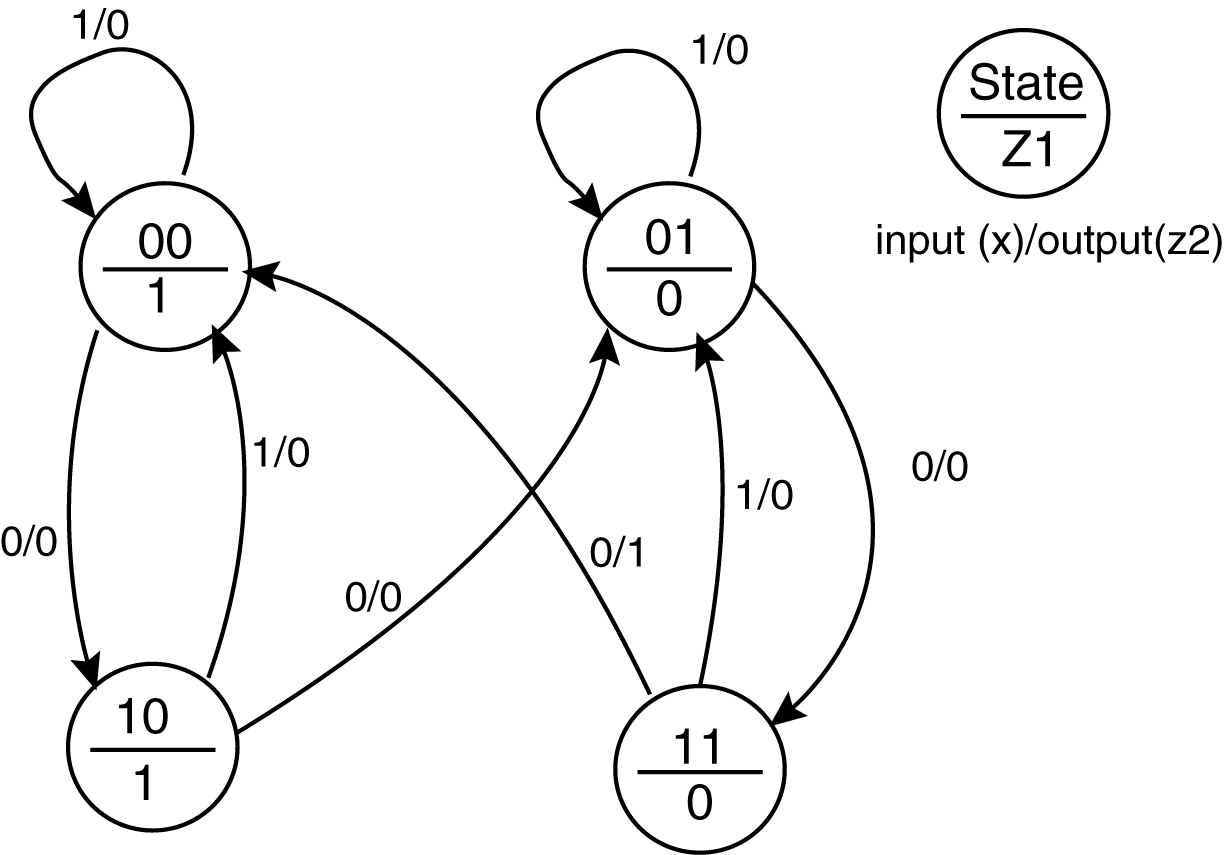
\includegraphics[width=6cm]{fsm/sm_ex6.png}
\end{minipage}

%%%%%% EXERCISE 7 %%%%%%
\vspace{20pt}
\noindent
\begin{minipage}{1\textwidth}
\textbf{EXERCISE 7.}
Draw the state diagram that corresponds to the following VHDL model and state whether the FSM is a Mealy machine or a Moore machine. Be sure to label everything.
\vspace{10pt}
\end{minipage}
\begin{minipage}{0.66\textwidth}

\begin{lstlisting}
-- library declaration
library IEEE;
use IEEE.std_logic_1164.all;
-- entity
entity fsm is
    Port ( CLK,CLR,SET,X1,X2 : in  std_logic;
                       Z1,Z2 : out std_logic);
end fsm;
-- architecture
architecture my_fsm of fsm is
   type state_type is (sA,sB,sC,sD); 
   attribute ENUM_ENCODING: STRING; 
   attribute ENUM_ENCODING of state_type: type is "1000 0100 0010 0001";
   signal PS,NS : state_type; 
begin
   sync_p: process (CLK,NS,CLR,SET) -- process
   begin
      if (CLR = '1' and SET = '0') then 
         PS <= sA; 
	  elsif (CLR = '0' and SET = '1') then 
	     PS <= sD;
      elsif (rising_edge(CLK)) then   
         PS <= NS; 
      end if; 
   end process sync_p; 

   comb_p: process (X1,X2,PS) -- process
   begin
      case PS is 
         when sA =>  
            if ( X1 = '1')  then 
               Z1 <= '0'; Z2 <= '0';   
               NS <= sA; 
            else  
               Z1 <= '0'; Z2 <= '0';   
               NS <= sB; 
            end if; 
         when sB =>
            if ( X2 = '1')  then 
               Z1 <= '1'; Z2 <= '1';   
               NS <= sC; 
            else  
               Z1 <= '1'; Z2 <= '0';   
               NS <= sB; 
            end if;				
         when sC =>
            if ( X2 = '1')  then 
               Z1 <= '0'; Z2 <= '0';   
               NS <= sB; 
            else  
               Z1 <= '0'; Z2 <= '1';   
               NS <= sC; 
            end if;
         when sD =>
            if ( X1 = '1')  then 
               Z1 <= '1'; Z2 <= '1';   
               NS <= sD; 
            else  
               Z1 <= '1'; Z2 <= '1';   
               NS <= sC; 
            end if;				
      end case; 
   end process comb_p; 
end my_fsm;
\end{lstlisting}
\end{minipage}
\begin{minipage}{0.29\textwidth}
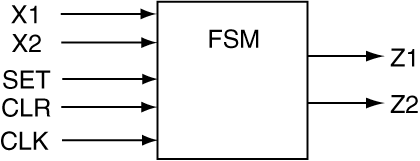
\includegraphics[width=4cm]{fsm/sm_ex7.png}
\vspace{250px}
\end{minipage}

%%%%%% EXERCISE 8 %%%%%%
\vspace{20pt}
\noindent
\begin{minipage}[t]{0.5\textwidth}
\textbf{EXERCISE 8.}
Write the VHDL behavioral model code that can be used to implement the state diagram shown on the right. The state variables should be encoded as listed and also provided as outputs of the FSM.
\end{minipage}
\begin{minipage}[t]{0.47\textwidth}
\vspace{0pt}\raggedright
\centering
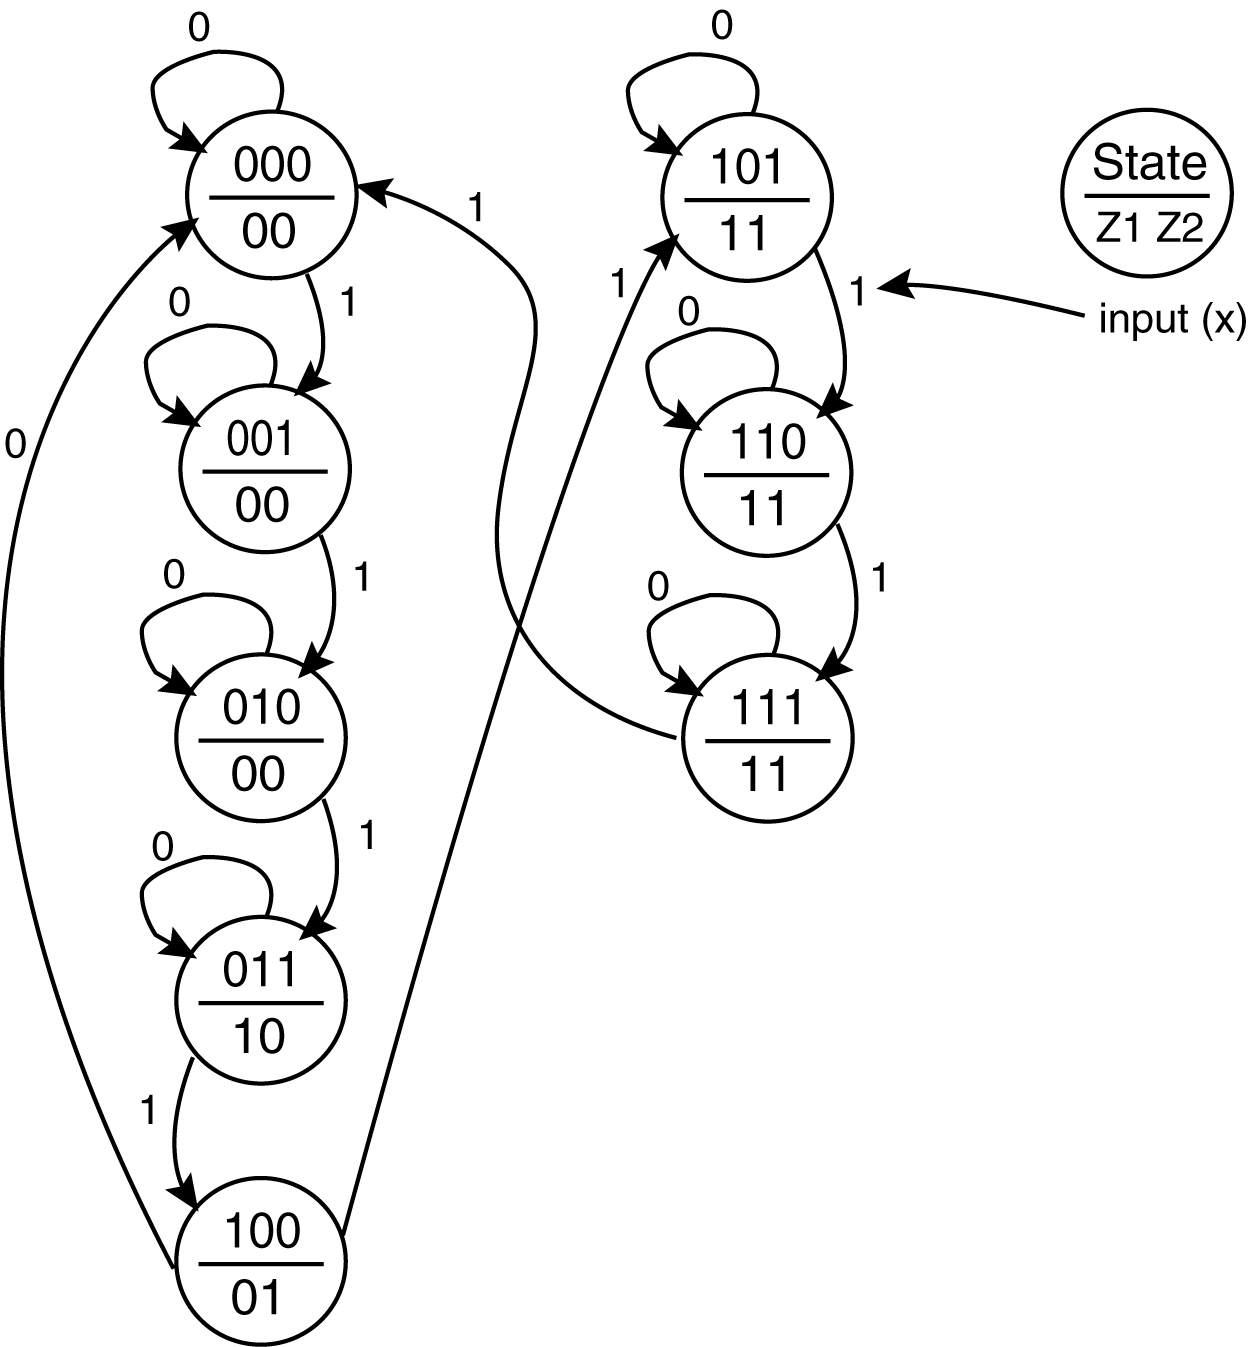
\includegraphics[width=5.3cm]{fsm/sm_ex8.png}
\end{minipage}

%%%%%% EXERCISE 9 %%%%%%
\vspace{20pt}
\noindent
\begin{minipage}[t]{0.5\textwidth}
\textbf{EXERCISE 9.}
Write the VHDL behavioral model code that can be used to implement the state diagram shown on the right. The state variables should be encoded as listed and also provided as outputs of the FSM.
\end{minipage}
\begin{minipage}[t]{0.47\textwidth}
\vspace{0pt}\raggedright
\centering
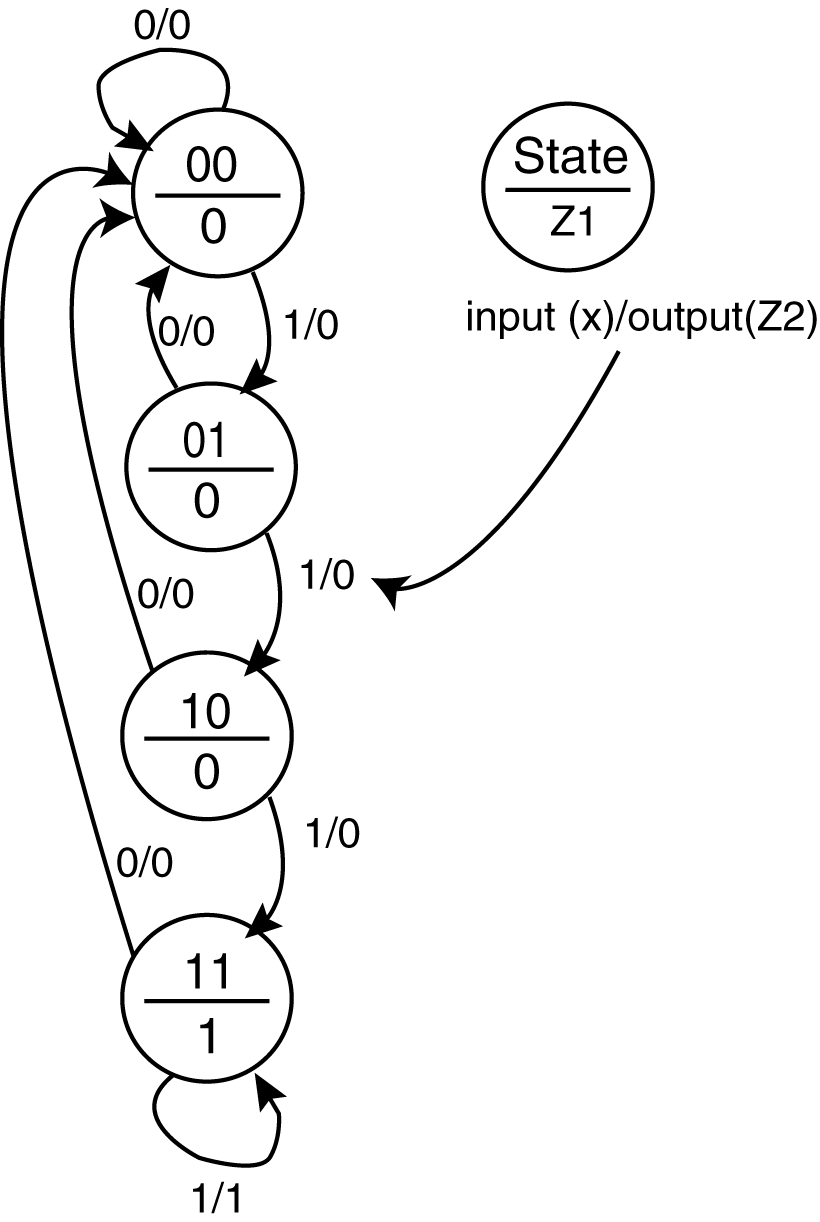
\includegraphics[width=4.2cm]{fsm/sm_ex9.png}
\end{minipage}

%%%%%% EXERCISE 10 %%%%%%
\vspace{20pt}
\noindent
\begin{minipage}[t]{0.5\textwidth}
\textbf{EXERCISE 10.}
Write the VHDL behavioral model code that can be used to implement the state diagram shown on the right. The state variables should be encoded as listed and also provided as outputs of the FSM.
\end{minipage}
\begin{minipage}[t]{0.47\textwidth}
\vspace{0pt}\raggedright
\centering
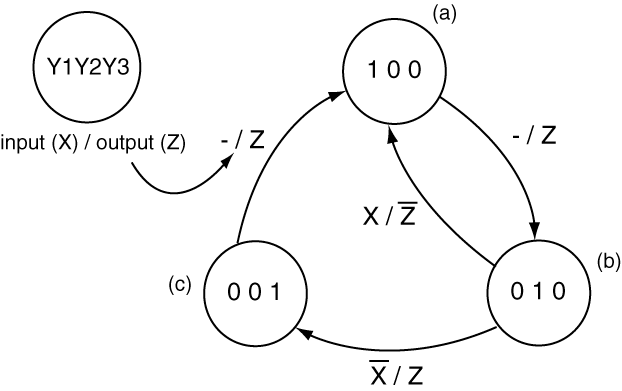
\includegraphics[width=6cm]{fsm/sm_ex10.png}
\end{minipage}

%%%%%% EXERCISE 11 %%%%%%
\vspace{20pt}
\noindent
\begin{minipage}[t]{0.5\textwidth}
\textbf{EXERCISE 11.}
Write the VHDL behavioral model code that can be used to implement the state diagram shown on the right. The state variables should be encoded as listed and also provided as outputs of the FSM.
\end{minipage}
\begin{minipage}[t]{0.47\textwidth}
\vspace{0pt}\raggedright
\centering
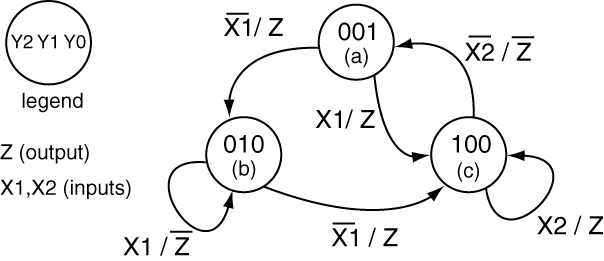
\includegraphics[width=6.4cm]{fsm/sm_ex11.png}
\end{minipage}

%%%%%% EXERCISE 12 %%%%%%
\vspace{20pt}
\noindent
\begin{minipage}[t]{1\textwidth}
\textbf{EXERCISE 12.}
Write the VHDL behavioral model code that can be used to implement the state diagram shown on the right. The state variables should be encoded as listed and also provided as outputs of the FSM.
\end{minipage}
\begin{minipage}[t]{1\textwidth}
\vspace{10pt}
\centering
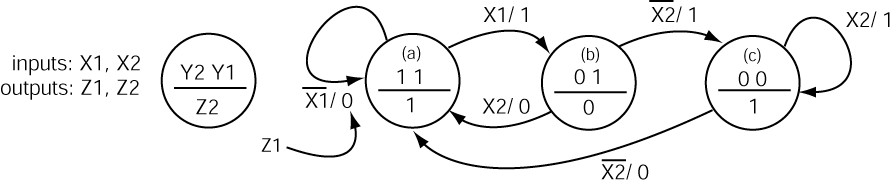
\includegraphics[width=11cm]{fsm/sm_ex12.png}
\end{minipage}

%%%%%% EXERCISE 13 %%%%%%
\vspace{20pt}
\noindent
\begin{minipage}[t]{0.5\textwidth}
\textbf{EXERCISE 13.}
Write the VHDL behavioral model code that can be used to implement the state diagram shown on the right. The state variables should be encoded as listed and also provided as outputs of the FSM.
\end{minipage}
\begin{minipage}[t]{0.47\textwidth}
\vspace{0pt}\raggedright
\centering
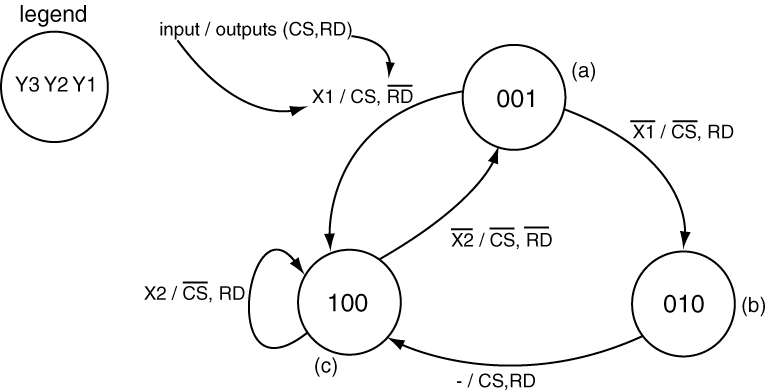
\includegraphics[width=6cm]{fsm/sm_ex13.png}
\end{minipage}

%%%%%% EXERCISE 14 %%%%%%
\vspace{20pt}
\noindent
\begin{minipage}[t]{0.5\textwidth}
\textbf{EXERCISE 14.}
Write the VHDL behavioral model code that can be used to implement the state diagram shown on the right. The state variables should be encoded as listed and also provided as outputs of the FSM.
\end{minipage}
\begin{minipage}[t]{0.47\textwidth}
\vspace{0pt}\raggedright
\centering
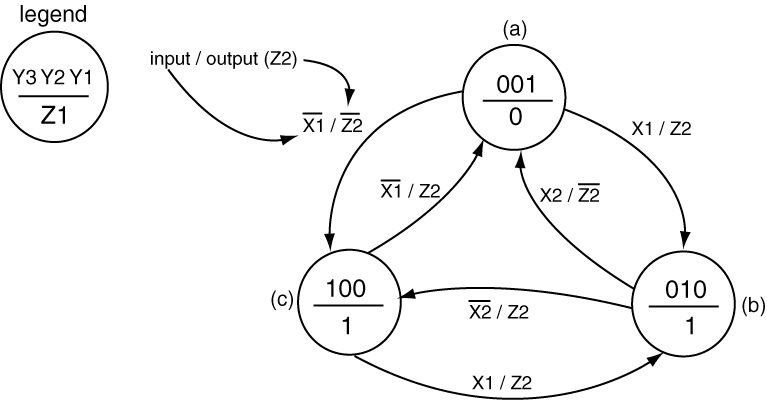
\includegraphics[width=6cm]{fsm/sm_ex14.png}
\end{minipage}




	% Free range VHDL
% Authors: Bryan Mealy, Fabrizio Tappero
% Date: May, 2012
% URL: freerangefactory.org
% (C) 2013 B. Mealy, F. Tappero
%
% !TEX root = master.tex
%
\chapter{Structural Modeling In VHDL}
As was mentioned earlier, there are generally three approaches to writing VHDL code: data-flow modeling, behavioral modeling and structural modeling.

Up to this point, this book has only dealt with data-flow and behavioral models. This section presents an introduction to structural modeling. 

As digital designs become more complex, it becomes less likely that any one design can be implemented with any one of the three types of VHDL models. We have already seen this property in dealings with FSMs where we mixed process statements (behavioral modeling) with selective signal assignment statements (data-flow modeling). The result was a hybrid VHDL model. By its very nature, structural modeling is likewise a hybrid VHDL model. Most complex designs could be considered structural models, i.e. if they are implemented using sound coding procedures. 

The design of complex digital circuits using VHDL should closely resemble the structure of complex computer programs. Many of the techniques and practices used to construct large and well structured computer programs written in higher-level languages should also be applied when using VHDL. This common structure we are referring to is the ever so popular modular approach to coding. The term structural modeling is the terminology that VHDL uses for the modular design. The VHDL modular design approach directly supports hierarchical design which is essentially employed when attempting to understand complex digital designs. 

The benefits of modular design to VHDL are similar to the benefits that modular design or object-oriented design provides for higher-level computer languages. Modular designs promote understandability by packing low-level functionality into modules. These modules can be easily reused in other designs thus saving the designer time by removing the need to reinvent and re-test the wheel. The hierarchical approach extends beyond code written on file level. VHDL modules can be placed in appropriately named files and libraries in the same way as higher-level languages. Moreover, there are often libraries out there that contain useful modules that can only be accessed using a structural-modeling approach. Having access to these libraries and being fluent in their use will serve to increase your perception as a VHDL guru.

After all the commentary regarding complex designs, we present a few simple examples. Though the structural approach is most appropriately used in complex digital designs, the examples presented in this section are rather simplistic in nature. These examples show the essential details of VHDL structural modeling. It is up to the designer to conjure up digital designs where a structural modeling approach would be more appropriate. Keep in mind that your first exposure to structural modeling may be somewhat rough. Although there is some new syntax to become familiar with, once you complete a few structural designs, this new syntax becomes ingrained in your brain and it becomes second nature to apply where required.

The tendency at this juncture in your VHDL programming career is to use some type of schematic capture software instead of learning the structural modeling approach. The fact is that no one of consequence uses the schematic capture software except for tired old university professors who are more interested in selling books than they are in teaching modern approach to VHDL modeling. The funny part about this entire process is that the schematic capture software is a tool that allows you to visually represent circuits but in the end generates VHDL code (the only thing the synthesizer understands is VHDL code).

\section{VHDL Modularity with Components}
The main tool for modularity in higher-level languages such as C is the function. In other computer languages, similar modularity is accomplished through the use of methods, procedures and subroutines. The approach used in C is to 1) name the function interface you plan on writing (the function declaration), 2) code what the function will do (the function body), 3) let the program know it exists and is available to be called (the prototype) and 4) call the function from the main portion of the code. In VDHL modularity is achieved via the use of \textbf{packages}, \textbf{components} and \textbf{functions}. In the following sections we are going to see how to use \texttt{components}.

The approach to use a \texttt{component} in VHDL  is: 1) name the module you plan to describe (the entity), 2) describe what the module will do (the architecture), 3) let the program know the module exists and can be used (component declaration) and 4) use the module in your code (component instantiation, or mapping). The similarities between these two approaches are listed in Table \ref{vhdl_c_comp}.

\begin{table}[!b]
\centering
\footnotesize\textsf{\begin{tabular}{ l l }
\hline
\rowcolor{gray} \textbf{C programming language} & \textbf{VHDL}\\
\hline
\rowcolor{light-gray} Describe function interface & The entity\\
\hline
Describe what the function does (coding) & The architecture \\
\hline
\rowcolor{light-gray} Provide a function prototype to main program & Component declaration \\
\hline
Call the function from main program & Component instantiation or mapping \\
\hline
\end{tabular}}
\caption{Similarities between modules in C and VHDL.}
\label{vhdl_c_comp}
\end{table}

Let us now use these principles in a practical example. Our approach is to describe a template-type approach to VHDL structural design using a simple and well-known combinational circuit.

\begin{leftbar}
\begin{minipage}[t]{0.52\textwidth}
\vspace{10pt}
\noindent
\textbf{EXAMPLE 22.}
Design a 3-bit comparator using a VHDL structural modeling. The interface to this circuit is described in the diagram below.
\end{minipage}
\begin{minipage}[t]{0.47\textwidth}
\vspace{0pt}\raggedright
    \centering
	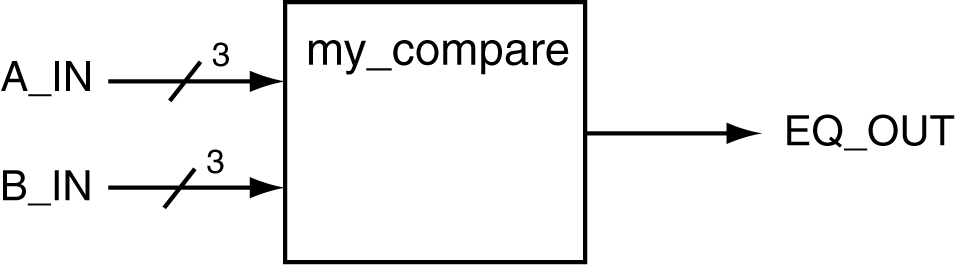
\includegraphics[width=5.2cm]{smu_vhdl/ex22.png}
\end{minipage}
\end{leftbar}

\noindent
\textbf{SOLUTION.} A comparator is one of the classic combinatorial circuits that every digital design engineer must derive at some point in his career. The solution presented here implements the discrete gate version of the circuit which is shown in Fig.~\ref{ex22_comp}. Once again, the solution presented here is primarily an example of a VHDL structural model and does not represent the most efficient method to represent a comparator using VHDL. 

The approach of this solution is to model each of the discrete gates as individual blocks. In this case, they are actually simple gates but the interfacing requirements of the VHDL structural approach are the same regardless of whether the circuit elements are simple gates or complex digital subsystems.

The circuit shown in Fig.~\ref{ex22_comp} contains some extra information that relates to its VHDL structural implementation. First, the dashed line represents the boundary of the top-level VHDL entity; therefore signals that cross this boundary must appear in the entity declaration for this implementation. Second, each of the internal signals is given a name. In this case, internal signals are defined to be signals that do not cross the dashed entity boundary. This is a requirement for VHDL structural implementations as these signals must be assigned to the various sub-modules in the interior of the design (somewhere in the architecture). 

\begin{figure}[!h]
    \centering
	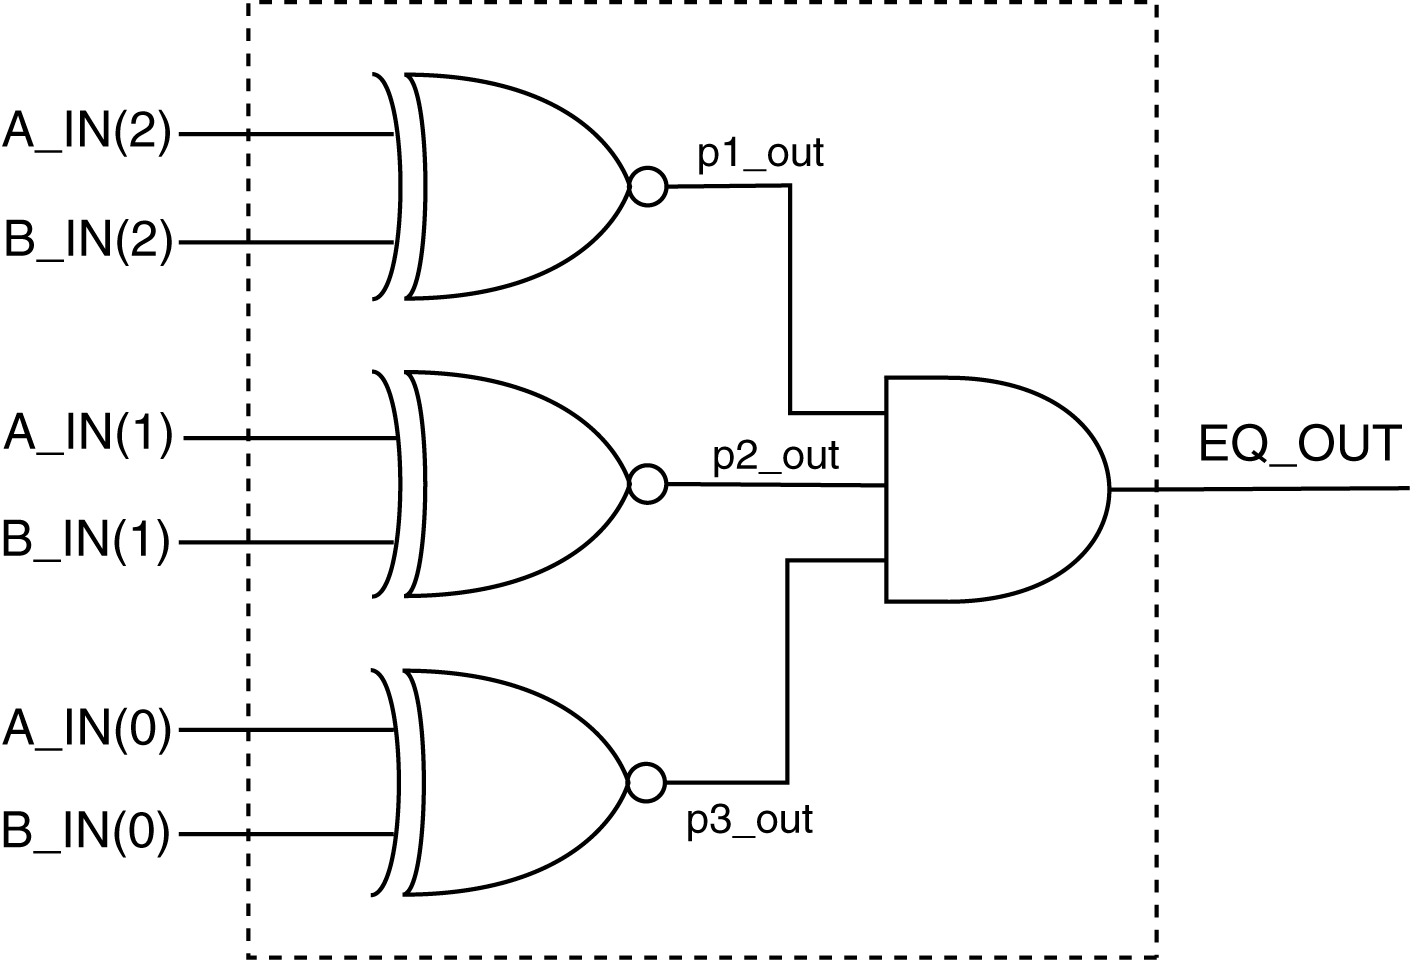
\includegraphics[width=7cm]{smu_vhdl/ex22_comp.png}
	\caption{Discrete gate implementation of a 3-bit comparator.}
	\label{ex22_comp}
\end{figure}

The first part of the solution is to provide entity and architecture implementations for the individual gates shown in Fig.~\ref{ex22_comp}. We need to provided as least one definition of an XNOR gate and a 3-input AND gate. We only need to provide one definition of the XNOR gate despite the fact that actually three are shown in the diagram. The modular VHDL approach allows us to reuse circuit definitions and we take advantage of this feature. These definitions are shown in Listing~\ref{ex22_code}. 

\noindent
\begin{minipage}{0.99\linewidth}
\begin{lstlisting}[label=ex22_code, caption=Entity and Architecture definitions for discrete gates.]
----------------------------------
-- Description of XNOR function --
----------------------------------
entity big_xnor is
    Port ( A,B : in  std_logic;
             F : out std_logic);
end big_xnor;

architecture ckt1 of big_xnor is
begin
      F <= not ( (A and (not B)) or ( (not A) and B) ); 
end ckt1;   
-----------------------------------------
-- Description of 3-input AND function --
-----------------------------------------
entity big_and3 is
    Port ( A,B,C : in std_logic;
               F : out std_logic);
end big_and3;

architecture ckt1 of big_and3 is
begin
      F <= ( A and B and C ); 
end ckt1;
\end{lstlisting}
\end{minipage}

The implementations shown in Listing~\ref{ex22_code} present no new VHDL details. The new information is contained in how the circuit elements listed in Fig.~\ref{ex22_comp} are used as components in a larger circuit. The procedures for implementing a structural VHDL design can be summarized in the following steps. These steps assume that the entity declarations for the interior modules already exist.

\noindent
\textbf{Step 1.} Generate the top-level entity declaration.\\
\textbf{Step 2.} Declare the lower-level design units used in design.\\
\textbf{Step 3.} Declare required internal signals used to connect the design units.\\
\textbf{Step 4.} Instantiate the design units.

This is how you therefore proceed:

\noindent
\textbf{Step One:} The first step in a structural implementation is identical to the standard approach we have used for the implementing other VHDL circuits: the \texttt{entity}. The entity declaration is derived directly from dashed box in Fig.~\ref{ex22_comp} and is shown in Listing~\ref{ex22_code_ent}. In other words, signals that intersect the dashed lines are signals that are known to the outside world and must be included in the entity declaration.

\noindent
\begin{minipage}{0.99\linewidth}
\begin{lstlisting}[label=ex22_code_ent, caption=Entity declaration for 3-bit comparator.]
-----------------------------------------------
-- Interface description of 3-bit comparator --
-----------------------------------------------
entity my_compare is
    Port ( A_IN   : in  std_logic_vector(2 downto 0);
           B_IN   : in  std_logic_vector(2 downto 0);
           EQ_OUT : out std_logic);
end my_compare;
\end{lstlisting}
\end{minipage}

\noindent
\textbf{Step Two:} The next step is to declare the design units that are used in the circuit. In VHDL lingo, declaration refers to the act of making a particular design unit available for use in a particular design. Note that the act of declaring a design unit, by definition, transforms your circuit into a hierarchical design. The declaration of a design unit makes the unit available to be placed into the design hierarchy. Design units are essentially modules that reside in the lower levels of the design. For our design, we need to declare two separate design units: the XOR gate and a 3-input AND gate.  

There are two factors involved in declaring a design unit: 1) how to do it and, 2) where to place it. A component declaration can be viewed as a modification of the associated entity declaration. The difference is that the word \texttt{entity} is replaced with the word \texttt{component} and the word \texttt{component} must also be followed by the word \texttt{end component} to terminate the declaration. The best way to do this is by copying, pasting and modifying the original entity declaration. The resulting component declaration is placed in the architecture declaration after the \texttt{architecture} line and before the \texttt{begin} line. The two component declarations and their associated entity declarations are shown in the next listing. Listing~\ref{ex22_code_final} shows the component declarations as they appear in working VHDL code.

\noindent
\begin{minipage}[t]{0.48\textwidth}
\vspace{0pt}
\noindent
\begin{lstlisting}[]

entity big_xnor is
    Port ( A,B : in  std_logic;
             F : out std_logic);
end big_xnor;
\end{lstlisting}
\begin{lstlisting}[]

entity big_and3 is
    Port ( A,B,C : in  std_logic;
               F : out std_logic);
end big_and3;
\end{lstlisting}
\end{minipage}
\begin{minipage}[t]{0.48\textwidth}
\vspace{0pt}\raggedright
\begin{lstlisting}[]

component big_xnor 
   Port ( A,B : in  std_logic;
            F : out std_logic);
end component;
\end{lstlisting}
\begin{lstlisting}[]

component big_and3 
   Port ( A,B,C : in  std_logic;
              F : out std_logic);
end component;
\end{lstlisting}
\end{minipage}

\noindent
\textbf{Step Three:} The next step is to declare internal signals used by your design. The required internal signals for this design are the signals that are not intersected by the dashed line shown in Fig.~\ref{ex22_comp}. These three signals are similar to local variables used in higher-level programming languages in that they must be declared before they can be used in the design. These signals effectively provide an interface between the various design units that are instantiated in the final design. For this design, three signals are required and used as outputs of the XOR gates and as inputs to the AND gate. Internal signal declarations such as these appear with the component declarations in the architecture declaration after the  \texttt{architecture} line and before the  \texttt{begin} line. Note that the declaration of intermediate signals is similar to the signal declaration contained in the entity body. The only difference is that the intermediate signal declaration does not contain the mode specifier. We have previously dealt with intermediate signals in other sections of this book. Signal declarations are included as part of the final solution shown in Listing~\ref{ex22_code_final}.

\noindent
\textbf{Step Four:} The final step is to create instances of the required modules and map the instances of the various components in the architecture body. Technically speaking, as the word instantiation implies, the appearance of instances of design units is the main part of the instantiation process. In some texts, the process of instantiation includes what we have referred to as component declaration but we have opted not to do this here. The approach presented here is to have the declaration refer to the component declarations before the \texttt{begin} line while instantiation refers to the creation of individual instances after the \texttt{begin} line. The mapping process is therefore included in our definition of component instantiation.

The process of mapping provides the interface requirements for the individual components in the design. This mapping step associates external connections from each of the components to signals in the next step upwards in the design hierarchy. Each of the signals associated with individual components maps to either an internal or external signal in the higher-level design. Each of the individual mappings includes a unique name for the particular instance as well as the name of the original entity. The actual mapping information follows the VHDL key words of \texttt{port map}. All of this information appears in the final solution shown in Listing~\ref{ex22_code_final}.

One key point to note in the instantiation process is the inclusion of labels for all instantiated design units. Labels should always be used as part of design unit instantiation because the use of appropriate labels increases the understandability of your VHDL model. In other words, the proper choice of labels increases the self-describing nature of your design and is considered a good VHDL programming approach.

\noindent
\begin{minipage}{0.99\linewidth}
\begin{lstlisting}[label=ex22_code_final, caption=VHDL code for the design hierarchy for the 3-bit comparator.]
-- library declaration
library IEEE;
use IEEE.std_logic_1164.all;
-- entity
entity my_compare is
    Port ( A_IN   : in  std_logic_vector(2 downto 0);
           B_IN   : in  std_logic_vector(2 downto 0);
           EQ_OUT : out std_logic);
end my_compare;
-- architecture
architecture ckt1 of my_compare is

   -- XNOR gate --------------------
   component big_xnor is
      Port ( A,B : in  std_logic;
               F : out std_logic);
   end component;
 
   -- 3-input AND gate -------------
   component big_and3 is
      Port ( A,B,C : in  std_logic;
                 F : out std_logic);
   end component;

   -- intermediate signal declaration
   signal p1_out,p2_out,p3_out : std_logic; 

begin
   x1: big_xnor port map (A => A_IN(2),
                          B => B_IN(2),
                          F => p1_out); 

   x2: big_xnor port map (A => A_IN(1),
                          B => B_IN(1),
                          F => p2_out); 
  
   x3: big_xnor port map (A => A_IN(0),
                          B => B_IN(0),
                          F => p3_out); 
  
   a1: big_and3 port map (A => p1_out,
                          B => p2_out, 
                          C => p3_out,
                          F => EQ_OUT); 
end ckt1;
\end{lstlisting}
\end{minipage}

It is worth noting that the solution shown in Listing~\ref{ex22_code_final} is not the only approach to use for the mapping process. The approach shown in Listing~\ref{ex22_code_final} uses what is referred to as a \texttt{direct mapping} of components. In this manner, each of the signals in the interface of the design units are listed and are directly associated with the signals they connect to in the higher-level design by use of the $=>$ operator. This approach has several potential advantages: it is explicit, complete, orderly and allows signals to be listed in any order. The only possible downside of this approach is that it uses up more space in your VHDL source code. 

The alternative approach to mapping is to use \texttt{implied mapping}. In this approach, connections between external signals from the design units are associated with signals in the design unit by order of their appearance in the mapping statement. This differs from direct mapping because only signals from the higher-level design appear in the mapping statement instead. The association between signals in the design units and the higher-level design are implied by the ordering of the signal as they appear in the component or entity declaration. This approach uses less space in the source code but requires signals to be placed in the proper order. An alternative but equivalent architecture for the previous example using implied mapping is shown in Listing~\ref{ex22_code_final_alt}. 

To successfully simulate and synthesize the design shown in Listing~\ref{ex22_code_final}, the code of Listing~\ref{ex22_code} needs to be included in your VHDL project as well. It is normal practice to keep the two listings in two distinctive files. The same is true for the implementation of Listing~\ref{ex22_code_final_alt}.

\noindent
\begin{minipage}{0.99\linewidth}
\begin{lstlisting}[label=ex22_code_final_alt, caption=Alternative architecture for Example~22 using implied mapping.]
-- library declaration
library IEEE;
use IEEE.std_logic_1164.all;
-- entity
entity my_compare is
    Port ( A_IN   : in  std_logic_vector(2 downto 0);
           B_IN   : in  std_logic_vector(2 downto 0);
           EQ_OUT : out std_logic);
end my_compare;
-- architecture
architecture ckt2 of my_compare is 
   component big_xnor is
      Port ( A,B : in  std_logic;
               F : out std_logic);
   end component;

   component big_and3 is
      Port ( A,B,C : in  std_logic;
                 F : out std_logic);
   end component;
   signal p1_out,p2_out,p3_out : std_logic; 

begin
   x1: big_xnor port map (A_IN(2),B_IN(2),p1_out); 
   x2: big_xnor port map (A_IN(1),B_IN(1),p2_out); 
   x3: big_xnor port map (A_IN(0),B_IN(0),p3_out);   
   a1: big_and3 port map (p1_out,p2_out,p3_out,EQ_OUT); 
end ckt2;
\end{lstlisting}
\end{minipage}

Due to the fact that this design was relatively simple, it was possible to bypass one of the interesting issues that arises when using structural modeling. Often when dealing with structural designs, different levels of the design will contain the same signal name. The question arises as to whether the synthesizer is able to differentiate between the signal names across the hierarchy. VHDL synthesizers, like compilers for higher-level languages, are able to handle such instances. Signals with the same names are mapped according to the mapping presented in the component instantiation statement. Probably the most common occurrence of this is with clock signals. In this case, a component instantiation such as the one shown in Listing~\ref{ex22_code_same_sig} is both valid and commonly seen in designs containing a system clock. Name collision does not occur because the signal name on the left-hand side of the $=>$ operator is understood to be internal to the component while the signal on the right-hand side is understood to reside in the next level up in the hierarchy.

\noindent
\begin{minipage}{0.99\linewidth}
\begin{lstlisting}[label=ex22_code_same_sig, caption=Example~of the same signal name crossing hierarchical boundaries.]
x5: some_component port map (CLK => CLK,
                              CS => CS); 
\end{lstlisting}
\end{minipage}


\section{Generic Map}
As we have seen in the previous section, the use of the keyword \texttt{component} allows us to declare a VHDL module for further instantiation.

Often it is desirable to write code that is generic. For instance a routine that perform a certain task on an input array of a generic size. Let us suppose that we want to implement a piece of code of a parity check routine that returns \texttt{'1'} when the input N-size array is an even number and \texttt{'0'} when the input N-size array is an odd number. The Listing~\ref{gen_parity_check} shows such an implementation.

\noindent
\begin{minipage}{0.99\linewidth}
\begin{lstlisting}[numbers=left, label=gen_parity_check, caption= Parity check implementation with generic input array size.]
-- library declarations
library IEEE;
use IEEE.std_logic_1164.all;
-- entity
entity gen_parity_check is
    generic ( n: positive);
    port    ( x: in  std_logic_vector(n-1 downto 0);
              y: out std_logic);
end gen_parity_check;
-- architecture
architecture arch of gen_parity_check is
    begin
        process(x)
            variable temp: std_logic;
        begin
            temp:='0';
            for i in x'range loop
                temp := temp XOR x(i);
            end loop;
            y <= temp;
        end process;
end arch;
\end{lstlisting}
\end{minipage}

Listing~\ref{gen_map} shows how the code above can be declared and instantiated in your own code via the already see \texttt{component} method. Specifically, In Listing~\ref{gen_map} the above generic parity check module is used to create a 4-bit parity check module.

To achieve the mentioned modularity the keyword \texttt{generic} was used inside the \texttt{entity} field in the code above and again inside the \texttt{component} field during its declaration in the code below. The \texttt{generic} field it is used to allow you to control all generic variables.

Notice how during instantiation, Listing~\ref{gen_map} line 20, the keyword \texttt{generic map} was used in conjunction with the keyword \texttt{port map} to define the generic variables.

\noindent
\begin{minipage}{0.99\linewidth}
\begin{lstlisting}[numbers=left, label=gen_map, caption=Use of \texttt{generic} for the construct of a generic parity check code.]
-- library declaration
library IEEE;
use IEEE.std_logic_1164.all;
-- entity
entity my_parity_chk is
    Port ( input   : in  std_logic_vector(3 downto 0);
           output  : out std_logic);
end my_parity_chk;

-- architecture
architecture arch of my_parity_chk is 
   --------------- component declaration --------------------
   component gen_parity_check is
      generic ( std_logic : positive);
      port    ( input     : in  std_logic_vector(N-1 downto 0);
                output    : out std_logic);
   end component;
begin
   -------------- component instantiation -------------------
   cp1: my_parity_chk generic map (4) port map (input, output);
end arch;

\end{lstlisting}
\end{minipage}

Once again, to successfully simulate and synthesize the design shown in Listing~\ref{gen_map}, the code of Listing~\ref{gen_parity_check} needs to be included in your VHDL project as well.

\section{Important Points}
\begin{my_list}
\item Structural modeling in VHDL supports hierarchical design concepts. The ability to abstract digital circuits to higher levels is the key to understanding and designing complex digital circuits.

\item Digital design using schematic capture is an outdated approach: you should resist the inclination and/or directive at all costs.

\item The VHDL structural model supports the reuse of design units. This includes units you have previously designed as well as the ability to use predefined module libraries.

\item If you use one FPGA software development tool from one of the major FPGA players in the market, you will be able to use digital blocks already developed once you declare them. In this case the entity declaration is not the one of Listing~\ref{ex22_code_ent} but instead a simple library inclusion in your VHDL code that looks like:

\vspace*{5pt}
\noindent
\begin{minipage}{0.99\textwidth}
\texttt{library UNISIM;}\\
\texttt{use UNISIM.VComponents.all;}\\
\end{minipage}
All digital blocks available from this library package are described in the documentation of the FPGA software development tool (e.g. Xilinx ISE).
\end{my_list}

\section{Exercises: Structural Modeling}

%%%%%% EXERCISE 1 %%%%%%
\vspace{20pt}
\noindent
\begin{minipage}{1\textwidth}
\textbf{EXERCISE 1.}
Draw a block diagram of the circuit represented by the VHDL code listed below. Be sure to completely label the final diagram.
\vspace{10pt}

\begin{lstlisting}
-- library declaration
library IEEE;
use IEEE.std_logic_1164.all;
-- entity
entity ckt1 is
    Port ( EN1, EN2 : in  std_logic;
                CLK : in  std_logic;
                  Z : out std_logic);
end ckt1;
-- architecture
architecture arch of ckt1 is

    component T_FF
        port ( T,CLK : in  std_logic;
                   Q : out std_logic);
    end component;

    signal t_in, t1_s, t2_s : std_logic;
begin
    t1 : T_FF
    port map (T => t_in,
            CLK => CLK,
              Q => t1_s );
    t2 : T_FF
    port map (T => t1_s,
            CLK => CLK,
              Q => t2_s );

       Z <= t2_s OR t1_s;
    t_in <= EN1 AND EN2;
end arch;
\end{lstlisting}
\end{minipage}

%%%%%% EXERCISE 2 %%%%%%
\vspace{20pt}
\noindent
\begin{minipage}{1\textwidth}
\textbf{EXERCISE 2.}
Draw a block diagram of the circuit represented by the VHDL code listed below. Be sure to completely label the final diagram.
\vspace{10pt}

\begin{lstlisting}
-- library declaration
library IEEE;
use IEEE.std_logic_1164.all;
-- entity
entity ckt is
    port ( A,B : in  std_logic;
             C : out std_logic);
end ckt;
-- architecture
architecture my_ckt of ckt is

    component bb1
        port (D,E : in  std_logic;
            F,G,H : out std_logic);
end component;

    component bb2
        port ( L,M,N : in  std_logic;
                   P : out std_logic);
end component;

    signal x1,x2,x3 : std_logic;
begin
    b1: bb1
    port map ( D => A, E => B, F => x1, G => x2, H => x3);

    b2: bb2
    port map ( L => x1, M => x2, N => x3, P => C);

end my_ckt;
\end{lstlisting}
\end{minipage}

%%%%%% EXERCISE 3 %%%%%%
\vspace{20pt}
\noindent
\begin{minipage}{\textwidth}
\textbf{EXERCISE 3.}
Provide the VHDL structural models for the circuits listed below.

\vspace{7pt}
\begin{minipage}[b]{0.45\linewidth}
\centering
a)
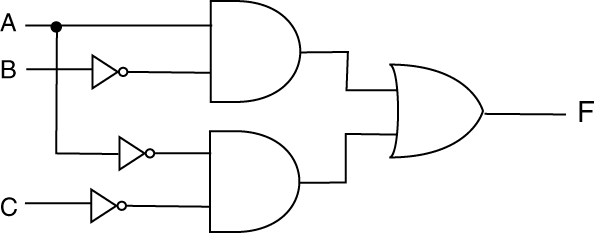
\includegraphics[width=0.8\textwidth]{smu_vhdl/ex3a.png}
\end{minipage}
\hspace{0.2cm}
\begin{minipage}[b]{0.5\linewidth}
\centering
b)
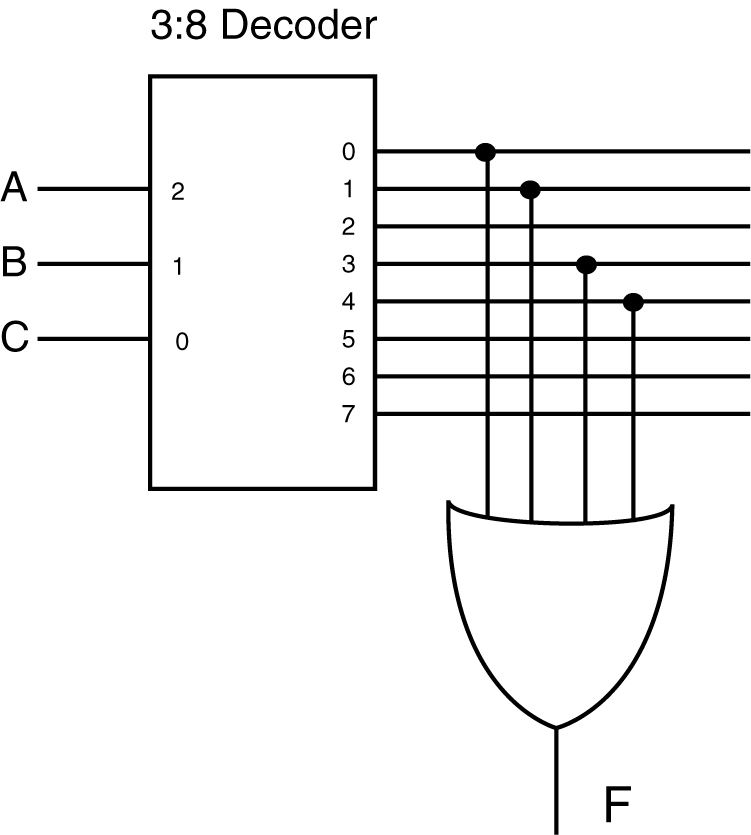
\includegraphics[width=0.5\textwidth]{smu_vhdl/ex3b.png}
\end{minipage}\\

\vspace{7pt}
\begin{minipage}[b]{0.45\linewidth}
\centering
c)
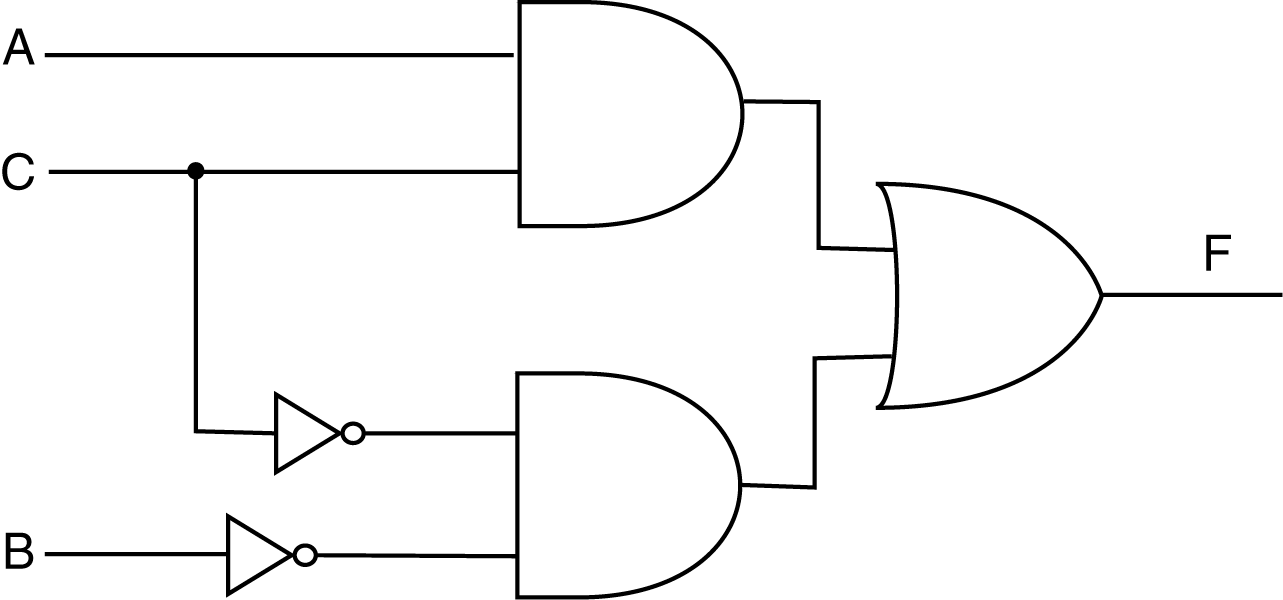
\includegraphics[width=0.8\textwidth]{smu_vhdl/ex3c.png}
\end{minipage}
\hspace{0.2cm}
\begin{minipage}[b]{0.5\linewidth}
\centering
d)
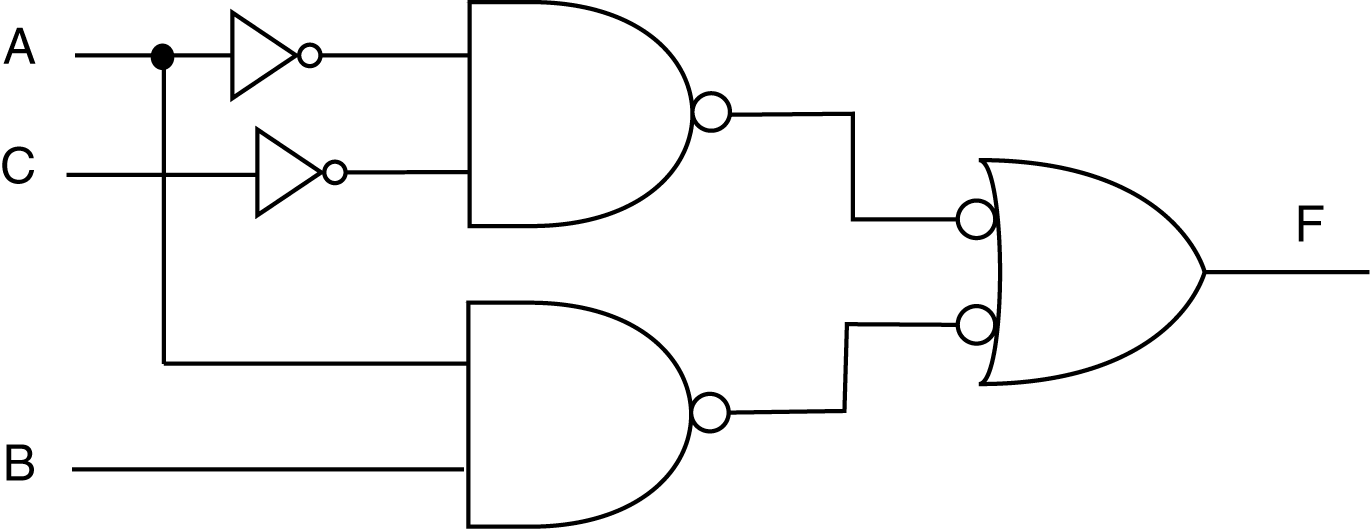
\includegraphics[width=0.8\textwidth]{smu_vhdl/ex3d.png}
\end{minipage}
\end{minipage}












	% Free range VHDL
% Authors: Bryan Mealy, Fabrizio Tappero
% Date: May, 2011
%
% (C) 2011 B. Mealy, F. Tappero
%
% !TEX root = master.tex
%
\chapter{Registers and Register Transfer Level}
The concept of a register in VHDL and its subsequent use in digital circuit design is probably one of the more straightforward concepts in VHDL. A register is VHDL is simply a vector version of a D flip-flop in which all operations on the flip-flops occur simultaneously. The "register transfer level", or RTL, is a flavor of design that is primarily concern with how and when data is transferred between the various registers in a digital system. RTL-level design in often associated with "data-path" designs which requires the careful control and timing of the data that is being transferred between registers. The controls associated with even simple registers are sufficient to ensure that some outside entity has adequate control over the "sequencing" of data through the circuit associated with the data-path. In these cases, the proper sequencing of data transfers is controlled by a FSM. 

The study of RTL-level design is best accomplished in the context of a data-path design. The design of data-paths is best accomplished in the context of a digital circuit that has some purpose such as an arithmetic logic unit design. Both of these topics are beyond what needs to be mentioned here. The good news is that the simplicity of the registers makes for a quick introduction to the matter. Major circuit implementations are saved for some other time.

\begin{leftbar}
\begin{minipage}[t]{0.52\textwidth}
\vspace{10pt}
\noindent
\textbf{EXAMPLE 23.}
Use VHDL behavioral modeling to design the 8-bit register that has a synchronous active high parallel load signal LD. Consider the load of the register to be synchronized to rising edges of the clock. 
\end{minipage}
\begin{minipage}[t]{0.47\textwidth}
\vspace{0pt}\raggedright
    \centering
	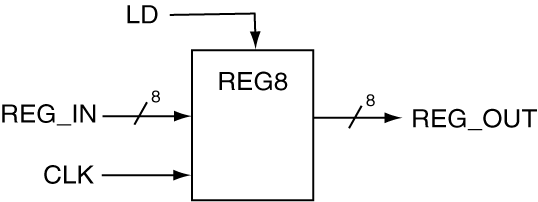
\includegraphics[width=5.2cm]{r_rtl/ex23.png}
\end{minipage}
\end{leftbar}
\noindent
\textbf{SOLUTION.} The solution for the 8-bit register looks amazingly similar to a model of a D flip-flop. The full solution to Example 23 is shown in listing \ref{ex23_code}. As usual, there are a couple of things worth noting in this solution.
\begin{my_list}
\item Note that there is an \texttt{if} statement that does not contain a corresponding \texttt{else} which is what generates the memory element. For this example, there are considered to be eight bit-sized memory elements (flip-flops). For this example the flip flops are considered to be D-type flip-flops. The storage elements are associated with the REG\_OUT bundle. The ease in using VHDL code to generate D flip-flops in this manner makes D flip-flops the most widely used type of flip-flop in digital design.

\item The code uses a bundle signal for both the input and output. The assignment of the bundles to other bundles is straightforward in VHDL as is shown in the code. In many cases, such as the one in this example, there is no need to use a bundle access operator in the VHDL model. 

\item The assignment of the input to the output is based on characteristics of both the clock edge and the state of the LD signal. The approach taken in the VHDL model shown in listing \ref{ex23_code} is to provide a separate \texttt{if} clause for both the LD and CLK signals. Only one \texttt{if} statement could have been used by making both conditions associated with the single \texttt{if} clause but this is not considered good VHDL programming practice when dealing with synchronized elements. In other words, you should always strive to keep special conditions associated with the clocking signal separate from all other conditions associated with the action in question. Clock signals are somewhat special in the VHDL land; you should get into the habit of treating them gently. 
\end{my_list}

\begin{lstlisting}[label=ex23_code, caption=Solution to Example 23.]
entity reg8 is
    Port ( REG_IN  :  in std_logic_vector(7 downto 0);
           LD,CLK  :  in std_logic;
           REG_OUT : out std_logic_vector(7 downto 0));
end reg8;

architecture reg8 of reg8 is
begin
   reg: process(LD,CLK,REG_IN)
   begin
      if (rising_edge(CLK)) then 
         if (LD = '1') then 
            REG_OUT <= REG_IN; 
         end if;
      end if;
   end process; 
end reg8;
\end{lstlisting}

The circuit in the following example is slightly more complex than most of the examples seen so far. Additionally, remember that there are many different solutions to the same problem. This is a common occurrence in VHDL, in fact, many times there is no best method for implementing a given circuit. The following examples are essentially the same problem solved using two different but functionally equivalent solutions.

\begin{leftbar}
\begin{minipage}[t]{0.5\textwidth}
\vspace{10pt}
\noindent
\textbf{EXAMPLE 24.}
Use VHDL behavioral modeling to design the circuit shown on the right. Consider both the loading signals to be active high. Consider the circuit to be synchronized to the rising edge of the clock signal. 
\end{minipage}
\begin{minipage}[t]{0.5\textwidth}
\vspace{0pt}\raggedright
    \centering
	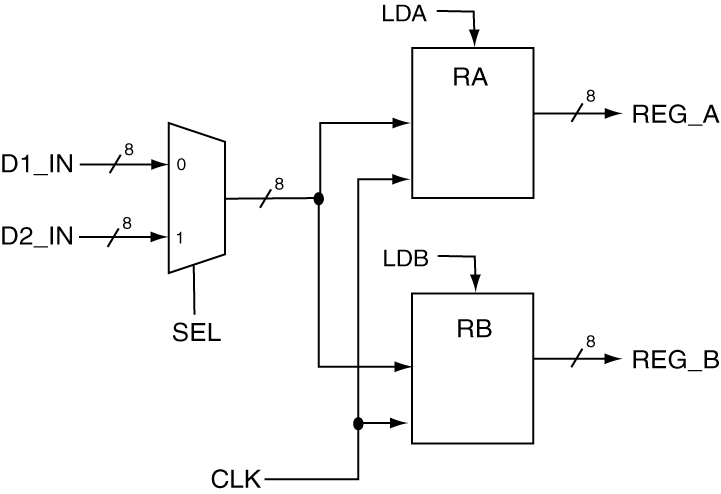
\includegraphics[width=5.7cm]{r_rtl/ex24.png}
\end{minipage}
\end{leftbar}
\noindent
\textbf{SOLUTION.} The circuit shown in Example 24 includes two 8-bit registers and a 2:1 MUX. This is an example of a bus-based data transfer in the output of the MUX that is connected to the inputs of the two registers. Each of the two registers has their own independent load control input. The solution to Example 24 is shown in listing \ref{ex23_code}. And as we have grown to expect, there are a couple of things worth noting about this solution. 
\begin{my_list}
\item There are three concurrent statements in this solution: two behavioral models and one data-flow model. 

\item There is a separate process for each of the two registers. Although it would have been possible to represent both registers using one process, it would have been somewhat complicated and somewhat hard to understand. The better approach in VHDL is always to break tasks down into their logically separate functions and use the various VHDL modeling techniques as tools to keep the tasks separate and simple. The reality is that the synthesizer becomes your friend if you provide it with simple models. The quantity of VHDL code describing a certain design is immaterial; the complexity of any given model is determined by the most complex piece of code in the model. Simple is always better in VHDL.

\item All of signal shown in the Example 24 have external linkage except for the output of the MUX. The MUX output is connected to the inputs of both registers. The final approach taken in this solution is typical in VHDL: many processes that communicate with each other through shared signals. In this example, there is only one shared signal but this is a fairly simple program. The same inter-process communication model is used in more complicated circuits.

\item The model for the 2:1 MUX uses the terminology \texttt{(others => '0')}. This is a short-hand terminology for assigning all of the outputs to '0'. The real nice part about this instruction is that you do not need to know how many 0’s you need to write. This is a nice feature in that if the width of the associated bundle were to change, this particular line of code would not need to be modified. 
\end{my_list}

\begin{lstlisting}[label=ex24_code, caption=Solution to Example 24.]
entity ckt_rtl is
   port (D1_IN,D2_IN : in std_logic_vector(7 downto 0);
             CLK,SEL : in std_logic; 
             LDA,LDB : in std_logic; 
         REG_A,REG_B : out std_logic_vector(7 downto 0)); 
end ckt_rtl; 

architecture rtl_behavioral of ckt_rtl is 
   -- intermediate signal declaration ---------------
   signal s_mux_result : std_logic_vector(7 downto 0);
begin

   ra: process(LDA,CLK,s_mux_result)
   begin
      if (rising_edge(CLK)) then 
         if (LDA = '1') then 
            REG_A <= s_mux_result; 
         end if;
      end if;
   end process; 
	
   rb: process(LDB,CLK,s_mux_result)
   begin
      if (rising_edge(CLK)) then 
         if (LDB = '1') then 
            REG_B <= s_mux_result; 
         end if;
      end if;
   end process; 
	
   with SEL select
   s_mux_result <= D1_IN when '1', 
                   D2_IN when '0', 
                   (others => '0') when others; 
end rtl_behavioral;
\end{lstlisting}

\begin{leftbar}
\begin{minipage}[t]{0.5\textwidth}
\vspace{10pt}
\noindent
\textbf{EXAMPLE 25.}
Use VHDL structural modeling to design the circuit shown on the right. Consider both of the loading signals to be active high. Consider the circuit to be synchronized to the rising edge of the clock signal.
\end{minipage}
\begin{minipage}[t]{0.5\textwidth}
\vspace{0pt}\raggedright
    \centering
	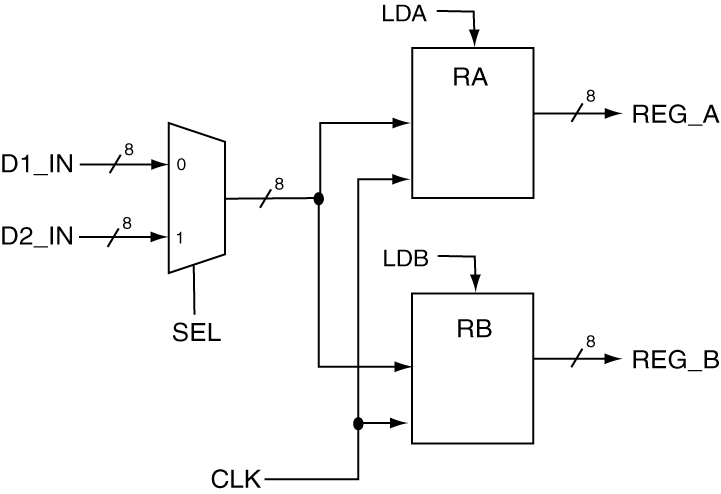
\includegraphics[width=5.7cm]{r_rtl/ex25.png}
\end{minipage}
\end{leftbar}
\noindent
\textbf{SOLUTION.} The solution to Example 25 is shown in listing \ref{ex25_code}. There is not too much interesting to note here. This is a more realistic example of a structural model compared to the example presented in the section on structural modeling. There are only a few new and wonderful things to note about this solution.

\begin{my_list}
\item The massively important thing to note about the solution in listing \ref{ex25_code} is to not be intimidated by the shear quantity of code listed. The code is well structured; if you are able to recognize this structure, you will be more apt to understand the solution. And better yet, you will be more on your way of being able to write you own amazing chunks of VHDL code. 

\item The VHDL source code shown in listing \ref{ex25_code} is nicely formatted. In particular, the code is nicely indented. Properly indented code is highly desirable in that it nicely presents information based on the indented. No surprise here but, properly formatted code is easier to understand. Better yet, good looking code leads people who may or may not know otherwise into thinking your code is as actually as good as it looks. In this busy world of ours, a quick glance is just about all the time people (bosses and teachers) have to dedicate to perusing your VHDL source code.
\end{my_list}

\begin{lstlisting}[label=ex25_code, caption=Solution to Example 25 using a structural modeling approach.]
entity mux2t1 is
   port (  A,B : in std_logic_vector(7 downto 0); 
           SEL : in  std_logic; 
         M_OUT : out std_logic_vector(7 downto 0)); 
end mux2t1; 

architecture my_mux of mux2t1 is
begin 
   with SEL select
   M_OUT <= A when '1', 
            B when '0', 
            (others => '0') when others; 
end my_mux;

entity reg8 is
    Port (  REG_IN : in std_logic_vector(7 downto 0);
            LD,CLK : in std_logic;
           REG_OUT : out std_logic_vector(7 downto 0));
end reg8;

architecture reg8 of reg8 is
begin
   reg: process(LD,CLK,REG_IN)
   begin
      if (rising_edge(CLK)) then 
         if (LD = '1') then 
            REG_OUT <= REG_IN; 
         end if;
      end if;
   end process; 
end reg8;

entity ckt_rtl is
   port (D1_IN,D2_IN : in std_logic_vector(7 downto 0);
             CLK,SEL : in std_logic; 
             LDA,LDB : in std_logic; 
         REG_A,REG_B : out std_logic_vector(7 downto 0)); 
end ckt_rtl; 

architecture rtl_structural of ckt_rtl is 
 
   -- component declaration -----------------------
   component mux2t1 
      port (  A,B : in std_logic_vector(7 downto 0); 
              SEL : in std_logic; 
            M_OUT : out std_logic_vector(7 downto 0)); 
   end component; 

   component reg8 
       Port (  REG_IN : in std_logic_vector(7 downto 0);
               LD,CLK : in std_logic;
              REG_OUT : out std_logic_vector(7 downto 0));
   end component;

   -- intermediate signal declaration ---------------
   signal s_mux_result : std_logic_vector(7 downto 0); 
	
begin
   ra: reg8
   port map ( REG_IN => s_mux_result,
                  LD => LDA,
                 CLK => CLK,
             REG_OUT => REG_A ); 

   rb: reg8
   port map ( REG_IN => s_mux_result,
                  LD => LDB,
                 CLK => CLK,
             REG_OUT => REG_B ); 
				 
   m1: mux2t1
   port map (   A => D1_IN, 
                B => D2_IN,
              SEL => SEL,
            M_OUT => s_mux_result); 				 
end rtl_structural;
\end{lstlisting}

\section{Important Points}

\begin{my_list}
\item VHDL can be used to easily implement circuits at the register transfer level. The corresponding VHDL models can be implemented in either structural of full behavioral format. 

\item RTL level VHDL models should strive for simplicity in their designs. If the behavioral models in the RTL design become complicated, the chances that your circuit works correctly greatly diminish due to the synthesis of the complicated circuit. 
\end{my_list}





	% Free range VHDL
% Authors: Bryan Mealy, Fabrizio Tappero
% Date: May, 2012
% URL: freerangefactory.org
% (C) 2013 B. Mealy, F. Tappero
%
% !TEX root = master.tex
%
\chapter{Data Objects}

Many of the concepts presented so far have been implicitly presented in the context of example problems. In this way, you have probably been able to generate quality VHDL code but were constrained to use the VHDL style presented in these examples. In this section, we will present some of the underlying details and theories that surround VHDL as a backdoor approach for presenting tools that will allow you to use VHDL for describing the behavior of more complex digital circuits.

In order to move into more sophisticated VHDL, a good place to start is with the definition of VHDL objects (e.g. data types). An object is an item in VHDL that has both a name (associated identifier) and a specific type. There are four types of objects and many different data types in VHDL. Up to this point, we have only used \texttt{signal} data objects and \texttt{std\_logic} data types. Two new data objects and several new data types are introduced and discussed in this section.

\section{Types of Data Objects}
There are four types of data objects in VHDL: \textbf{signals}, \textbf{variables}, \textbf{constants} and \textbf{files}. One of the purposes of this section is to present some background information regarding variables which will be used later in this tutorial. The idea of constants will also be briefly mentioned since they are generally straightforward to understand and use once the concepts of signals and variables are understood. File data objects, exclusively used in simulations, are not discussed in this chapter.

Mind that VHDL is a vast language that goes well beyond the VHDL code that is used to program an FPGA or a CPLD. In fact the actual VHDL that can be translated into an FPGA/CPLD bit-stream is called RTL VHDL and represents only a small subset of what is included in the current VHDL standard. The file  data objects are an example of a data object that cannot be implemented in a silicon device.

Just as side note, it is interesting to point out that it is also possible to compile VHDL code into an executable file that can be executed, generally for simulation purposes, with any general purpose Intel PC. For more details refer to the open-source work of T. Gingold available at:

\noindent
\url{http://ghdl.free.fr}.

\section{Data Object Declarations}

The first thing to note about data objects is the similarity in their declarations. The forms for the three data objects we will be discussing are listed in Table \ref{vhdl_data_objs}. For each of these declarations, the bold-face font is used to indicate VHDL keywords. The form for the signal object should seem familiar since we have used it extensively up to this point.

\begin{table}[!h]
\centering
\footnotesize\textsf{\begin{tabular}{ l l }
\hline
\rowcolor{gray} \textbf{VHDL data object} & \textbf{Declaration form}\\
\hline
\rowcolor{light-gray} Signal & \texttt{{\bf signal} sig\_name : sig\_type:=initial\_value;} \\
\hline
Variable & \texttt{{\bf variable} var\_name : var\_type:=initial\_value;} \\
\hline
\rowcolor{light-gray} Constant & \texttt{{\bf constant} const\_name : const\_type:=initial\_value;} \\
\hline
\end{tabular}}
\caption{Data object declaration forms.}
\label{vhdl_data_objs}
\end{table}

Note that each of the data objects can optionally be assigned initial values. Signal declarations do not usually include initial values as opposed to constants which generally do. 

Initial values for signals are in fact not implementable on silicon by the synthesizing tools but are taken into consideration by VHDL simulation tools. Example~declarations for these three flavors of data objects are provided in Table \ref{vhdl_data_objs_ex}. These examples include several new data types which will be discussed in the next section. 

\begin{table}[!h]
\centering
\footnotesize\textsf{\begin{tabular}{ l l }
\hline
\rowcolor{gray} \textbf{Data object} & \textbf{Declaration form}\\
\hline
Signal & \texttt{{\bf signal} sig\_var1 : std\_logic := '0';} \\
& \texttt{{\bf signal} tmp\_bus : std\_logic\_vector(3 downto 0):="0011";} \\
& \texttt{{\bf signal} tmp\_int : integer range -128 to 127 := 0;}  \\
& \texttt{{\bf signal} my\_int  : integer;}\\
\hline
Variable &\texttt{{\bf variable} my\_var1, my\_var2 : std\_logic;} \\
&\texttt{{\bf variable} index\_a : integer range (0 to 255) := 0;} \\ 
&\texttt{{\bf variable} index\_b : integer := -34;} \\
\hline
Constant & \texttt{{\bf constant} sel\_val : std\_logic\_vector(2 downto 0):="001";} \\
&\texttt{{\bf constant} max\_cnt : integer := 12;} \\
\hline
\end{tabular}}
\caption{Example~declarations for signal, variable and constant data objects.}
\label{vhdl_data_objs_ex}
\end{table}

\section{Variables and Assignment Operator ``\texttt{:=}''}
Although variables are similar to signals, variables are not as functional for the several reasons mentioned in this section. Variables can only be declared and used inside of processes, functions and procedures (functions and procedures will not be discussed here). Implied in this statement is the sequential nature of variable assignment statements in that all statements appearing in the body of a process are sequential. One of the early mistakes made by VHDL programmers is attempting to use variables outside of processes.

The signal assignment operator, $<=$, was used to transfer the value of one signal to another while dealing with signal data objects. When working with variables, the assignment operator $:=$ is used to transfer the value of one variable data object to another. As you can see from Table \ref{vhdl_data_objs_ex}, the assignment operator is overloaded which allows it to be used to assign initial values to the three listed forms of data objects.

\section{Signals vs. Variables}
The use of signals and variables can be somewhat confusing because of their similarities. Generally speaking, a signal can be thought of as representing a wire or some type of physical connection in a design. Signals thus represent a means to interface VHDL modules which include connections to the outside world. In terms of circuit simulation, signals can be scheduled to take on multiple values at specific times in the simulation. The specifics of simulating circuits using VHDL are not covered here so the last statement may not carry much meaning to you. The important difference here is that events can be scheduled for signals while for variables, they cannot. The assignment of variables is considered to happen immediately and cannot have a list of scheduled events.

With relatively simple circuits, signal objects are generally sufficient. As your digital designs become more complex, there is a greater chance that you will need more control of your models than signals alone can provide. The main characteristic of signals that leave them somewhat limited in complex designs is when and how they are scheduled. More specifically, \textbf{assignments made to signals inside a process are actually only scheduled when the same process is completed. The actual assignment is not made until after the process terminates}. This is why multiple signal assignments can be made to the same signal during the execution of a process without generating any type of synthesis error. In the case of multiple signal assignments inside the process, only the most recent assignment to the signal during process execution is assigned. The important thing here is that the signal assignment is not made until after the process terminates. The potential problem that you might face is that the new result (the new value assigned to the signal) is not available to use inside the process. 

Variable assignment within processes is different. When a variable is assigned a value inside of a process, the assignment is immediate and the newly assigned value can be used immediately inside of the process. In other words, the variable assignment is not scheduled as it was for the signal. This is a giant difference and has very important ramifications in both the circuit simulation and synthesis realm. 

Variables cannot always be modeled as wires in a circuit. They also have no concept of memory since they cannot store events. With all this in mind, you may wonder what is the appropriate place to use variables. The answer is variables should only be used as iteration counters in loops or as temporary values when executing an algorithm that performs some type of calculation. It is possible to use variables outside of these areas, but it should be avoided.

Even though instructions inside a process are executed consecutively, this should not fool you in thinking that a process environment is similar to a segment of C code. Remember that while lines of C code require some tens of clock cycles each to be executed, VHDL instructions require very little time to be executed, less than one clock cycle. The price to pay for this enormously fast execution time is that any signal assignment inside a process only takes place at the end of the process. It is therefore advisable that your processes are short and simple.

\section{Standard Data Types}
Not only does VHDL have many defined data types but VHDL also allows you to define your own types. Here however we will only deal with few of the most widely used types. Among the most popular VHDL data type we would like to mention the following data types:\\

\noindent
\texttt{bit}: It is a two-value enumerated type. Replaced by the \texttt{std\_logic} type.\\
\texttt{bit\_vector}: Replaced by the more powerful \texttt{std\_logic\_vector} type.\\
\texttt{boolean}: As expected, it is a two-value enumerated type.\\
\texttt{boolean vector}: It is the vector form of a \texttt{boolean} type.\\
\texttt{integer}: Refer to the Integer Types section.\\
\texttt{natural}: It is a subtype of \texttt{integer} because it is a non-negative integer.\\
\texttt{positive}: It is a subtype of \texttt{integer} because it is a positive integer.\\
\texttt{integer\_vector}: It is the vector form of an \texttt{integer} type.\\
\texttt{character}: A 256-symbol enumerated type.\\
\texttt{string}: It is the vector form of a \texttt{character} type.\\

In the following sections, a few more popular and useful types are introduced.

\section{User-Defined Types}
VHDL allows you to define your own data type. A typical example of a custom integer type is:

\noindent
\texttt{type my\_type is range 0 to 100;}\\
\texttt{constant my\_const : my\_type := 31;}

\noindent
Obviously it is possible to define more complex data structures. For instance it is a common practice to use a custom data type when you want to implement a ROM (read-only memory) in VHDL.

\noindent
\begin{minipage}{0.99\linewidth}
\begin{lstlisting}

-- typical custom data type for a 20-byte ROM
type memory is array (0 to 19 of std_logic_vector(7 downto 0);
constant my_rom : memory := (
        1 => "11111111"
        2 => "11110111"
        5 => "11001111"
       12 => "10110101"
       18 => "10001101"
   others => "00000000");
\end{lstlisting}
\end{minipage}

\section{Commonly Used Types}
The types already introduced in previous chapters as well as two new types are listed in Table \ref{vhdl_data_types}. The \texttt{std\_logic} and \texttt{std\_logic\_vector} types have been extensively used so far. These types are more complex than has been previously stated and will be discussed further in this chapter. The \texttt{enumerated} type was used during the previous discussion of finite state machines. The \texttt{integer} type was cryptically mentioned before but it will be discussed further along with the \texttt{boolean} type in this chapter. 

\begin{table}[!h]
\centering
\footnotesize\textsf{\begin{tabular}{ l l l}
\hline
\rowcolor{gray} \textbf{Type} & \textbf{Example} & \textbf{Usage} \\
\hline
\rowcolor{light-gray} std\_logic & \texttt{{\bf signal} my\_sig : {\bf std\_logic};} & all examples \\
\hline
std\_logic\_vectors & \texttt{{\bf signal} busA : {\bf std\_logic\_vector}(3 downto 0)}; & all examples \\
\hline
\rowcolor{light-gray} enumerated &  \texttt{{\bf type} state\_type {\bf is} (ST0,ST1,ST2,ST3);} & Example~18\\
\hline
boolean & \texttt{{\bf variable} my\_test : {\bf boolean} := {\bf false};} & None \\
\hline
\rowcolor{light-gray} integer & \texttt{{\bf signal} iter\_cnt : {\bf integer} := 0;}  & Example~26 \\
\hline
\end{tabular}}
\caption{Some popular data types already introduced in previous chapters.}
\label{vhdl_data_types}
\end{table}

\section{Integer Types}
The use of integer types aids in the design of algorithmic-type VHDL code. This type of coding allows VHDL to describe the behaviour of complex digital circuits. As you progress in your digital studies, you will soon find yourself in need of more complex descriptive VHDL tools. Data types such as integers partially fill that desire. This section briefly looks at integer types as well as the definition of user-specified integer types.

The range of the integer type is (-2,147,483,648 to 2,147,483,647). These numbers should seem familiar since they represent the standard 32-bit range for a signed number: from $-(2^{31})$ to $+(2^{31}-1)$. Other types similar to integers include natural and positive types. These types are basically integers with shifted ranges. For example, the natural and positive types range from 0 and 1 to the full 31-bit range, respectively. Examples of integer declarations are shown in the following listing.
\vspace{8pt}

\noindent
\begin{minipage}{0.99\linewidth}
\begin{lstlisting}

-- integer declarations
signal   my_int     : integer range 0 to 255 := 0;
variable max_range  : integer := 255;
constant start_addr : integer := 512;
\end{lstlisting}
\end{minipage}

Although it could be possible to use only basic integer declarations in your code, as we have seen before, VHDL allows you to define your own data types with their own personalized range constraints. These special types should be used wherever possible to make your code more readable. The custom integer-type definition uses the type \texttt{range} construct and the \texttt{to} or the \texttt{downto} keywords for the definition. Some examples of integer-type declarations are provided in the following listing.
\vspace{8pt}

\noindent
\begin{minipage}{0.99\linewidth}
\begin{lstlisting}

-- integer type declarations
type scores  is range 0 to 100; 
type years   is range -3000 to 3000; 
type apples  is range 0 to 15; 
type oranges is range 0 to 15; 
\end{lstlisting}
\end{minipage}

Although each of the types listed in the previous listing are basically integers, they are still considered different types and cannot be assigned to each other. In addition to this, any worthy VHDL synthesizer will do range checks on your integer types. In the context of the definitions previously presented, each of the statements in the following listing is illegal. 
\vspace{8pt}

\noindent
\begin{minipage}{0.99\linewidth}
\begin{lstlisting}

-- Illegal assignment statements
signal score1    : scores  := 100;  
signal my_apple  : apples  := 0; 
signal my_orange : oranges := 0; 

my_apple  <= my_orange;  -- different types
my_orange <= 24;         -- out of range
my_score  <= 110;        -- out of range
\end{lstlisting}
\end{minipage}

\section{\texttt{signed} and \texttt{unsigned} Types}
\texttt{signed} and \texttt{unsigned} data types are available once you declare the standard IEEE \texttt{ieee.numeric\_std} package. Mind that these two data types are also defined in the non-standard \texttt{std\_logic\_arith} package. The use of non-standard libraries is however highly discouraged.

A \texttt{signed} value ranges from $-2^{N-1}$ to $2^{N-1}-1$ and an \texttt{unsigned} value ranges from $0$ to $2^N-1$ where $N$ is the number of bits.

\texttt{signed} and \texttt{unsigned} types can be conveniently used for internal variables as well as for entity ports. Additionally the \texttt{ieee.numeric\_signed} library and the \texttt{ieee.numeric\_unsigned} library offer arithmetic and type conversion for both types.

\texttt{signed} and \texttt{unsigned} types, in a way, look like \texttt{std\_logic\_vector} types, especially in how they are declared and so the question that you might have is:
\begin{quotation}\ttfamily
Why would I need to use a \textbf{\color{gray}signed} or \textbf{\color{gray}unsigned} type in place of a \textbf{\color{gray}std\_logic\_vector} type?
\end{quotation}
The answer to this question is in Listing~\ref{my_sum}, specifically in line 17 and in line 18. The \texttt{std\_logic\_vector} type should not be used to define a numerically meaningful\footnote{Numerically meaningful signal: a signal that looks and behave like a number.} signal or variable. The \texttt{std\_logic\_vector} type should be only employed for defining ``bags of bits''.

The use of \texttt{signed/unsigned} types is desirable any time your bags of bits (signals, variables or constants) stop being ``bags'' and become numbers of type signed, unsigned or even integers.

\noindent
\begin{minipage}{0.99\linewidth}
\begin{lstlisting}[numbers=left, label=my_sum, caption= Use of unsigned types in your code.]
-- library declaration
library IEEE;
    use IEEE.std_logic_1164.all; -- defines std_logic_vector type
    use IEEE.numeric_std.all;    -- defines signed and unsigned types
-- entity
entity double_sum is
    Port (
        in1       : in  std_logic_vector (7 downto 0);
        in2       : in  std_logic_vector (7 downto 0);
        out1      : out std_logic_vector (7 downto 0));
        unsig_in  : in  unsigned(7 downto 0);
        unsig_out : out unsigned(7 downto 0));
    end double_sum;
-- architecture
architecture arch of sum is
    begin
        out1 <= in1 + 1;  -- ILLEGAL OPERATION, 1 is an integer
        out1 <= in1 + in2;-- ILLEGAL OPERATION, addition is not defined
        unsig_out <= unsig_in + 1;                  -- legal operation
        unsig_out <= unsigned(in1) + 1;             -- legal operation
        out1 <= std_logic_vector(unsigned(in1) + 1);-- legal operation
    end arch;
\end{lstlisting}
\end{minipage}

As final note, we should mention that the inclusion of the non-standard \texttt{std\_logic\_arith} library could have given us the possibility of doing \texttt{out1 <= in1 + 1;} in line 17 of Listing~\ref{my_sum}, making things much simpler. However, once again, the use of non-standard library is highly discouraged.

\section{\texttt{std\_logic} Types}
For the representation of digital signals so far in this book, we have used the \texttt{std\_logic} type. However, one of the data types, similar to \texttt{std\_logic}, neither used nor endorsed in this book is the \texttt{bit} type. This type can take on only the values of \texttt{'1'} or \texttt{'0'}. While this set of values seems appropriate for designing digital circuits, it is actually somewhat limited. Due to its versatility and a more complete range of possible values, the \texttt{std\_logic} type is preferred over \texttt{bit} types. The \texttt{std\_logic} type is defined in the VHDL package \texttt{ieee.std\_logic\_1164} and provides a common standard that can be used by all VHDL programmers.

The \texttt{std\_logic} type is officially defined as an \texttt{enumerated} type. Two of the possible enumerations of course include \texttt{'1'} and \texttt{'0'}. The actual definition is shown in the Listing~\ref{logic_type}. The \texttt{std\_logic} type is a resolved version of the \texttt{std\_ulogic} type. Resolved means that unlike for \texttt{std\_ulogic} types, when you use \texttt{std\_logic} type signals, you can use multiple assignments to the same signal without having the compile to complain about it.

\noindent
\begin{minipage}{0.99\linewidth}
\begin{lstlisting}[label=logic_type, caption=Declaration of the \texttt{std\_logic} enumerated type.]

type std_logic is  ( 'U', -- uninitialised 
                     'X', -- forcing unknown
                     '0', -- forcing 0
                     '1', -- forcing 1
                     'Z', -- high impedance
                     'W', -- weak unknown
                     'L', -- weak 0
                     'H', -- weak 1
                     '-'  -- unspecified (do not care) 
                   );
\end{lstlisting}
\end{minipage}

The \texttt{std\_logic} type uses the VHDL character type in its definition. Although there are nine values in the definition shown in Listing~\ref{logic_type}, this book only deals with \texttt{'0'},  \texttt{'1'},  \texttt{'Z'} and  \texttt{'-'}. The  \texttt{'Z'} is generally used when dealing with bus structures. This allows a signal or set of signals (a bus) to have the possibility of being driven by multiple sources without the need to generate resolution functions. When a signal is driven to its high-impedance state, the signal is not driven from that source and is effectively removed from the circuit. Finally, since the characters used in the \texttt{std\_logic} type are part of the definition, they must be used as listed. Mind the use of lower-case letters will generate an error. 
\begin{leftbar}
\begin{minipage}[t]{0.52\textwidth}
\vspace{10pt}
\noindent
\textbf{EXAMPLE 26.}
Design a clock divider circuit that reduces the frequency of the input signal by a factor of 64. The circuit has two inputs as shown in the diagram. The  \texttt{div\_en} input allows the  \texttt{clk} signal to be divided when asserted and the  \texttt{sclk} output will exhibit a frequency 1/64 that of the  \texttt{clk} signal. When  \texttt{div\_en} is not asserted, the  \texttt{sclk} output remains low. Frequency division resets when the  \texttt{div\_en} signal is reasserted.
\end{minipage}
\begin{minipage}[t]{0.4\linewidth}
\vspace{10pt}
\begin{flushright}
\begin{tikzpicture}
[x=1mm,y=1mm,line width=0.8pt,scale=1,framed]
% BOX
\draw (20,5) rectangle (35,20) node[midway]{$clk\_div$};
% INPUTS
\small
\node (b) at (0,-2) {}; % this is to extend the pink area
\node (b) at (20,22.5) {}; % this is to extend the pink area
\node (a) at (20,2.5) {}; % this is the reference point
\draw [latex-] ($(a)+(0,15)$) -- ++(-10,0) node[above]{clk};
\draw [latex-] ($(a)+(0,5)$) -- ++(-10,0) node[above]{div\_en};
% OUTPUTS
\draw [-latex] ($(a)+(15,10)$) -- ++(10,0) node[above]{sclk};
\end{tikzpicture}
\end{flushright}
\end{minipage}
\end{leftbar}
\noindent
\textbf{SOLUTION.} As usual for more complex concepts and circuits, there are a seemingly infinite number of solutions. A solution that uses several of the concepts discussed in this section is presented in Listing~\ref{ex26_code}. Some of the more important issues in this solution are listed below.

\begin{my_list}
\item The type declaration for  \texttt{my\_count} appears in the architecture body before the \texttt{begin} statement. 

\item A constant is used for the  \texttt{max\_count} variable. This allows for quick adjustments in the clock frequency. In this example, this concept is somewhat trivial because the  \texttt{max\_count} variable is used only once.  

\item The variable is declared inside of the process, after the process \texttt{begin} line.
\end{my_list}

\noindent
\begin{minipage}{0.99\linewidth}
\begin{lstlisting}[numbers=left,label=ex26_code, caption=Solution to Example~26.]

-- library declaration
library IEEE;
use IEEE.std_logic_1164.all;
use IEEE.numeric_std.all;

-- entity
entity clk_div is
Port (
    clk    : in  std_logic;
    div_en : in  std_logic;
    sclk   : out std_logic);
end clk_div;

-- architecture
architecture my_clk_div of clk_div is
    type my_count is range 0 to 100;     -- user-defined type
    constant max_count : my_count := 31; -- user-defined constant
    signal tmp_sclk : std_logic;         -- intermediate signal
    begin
        my_div: process (clk,div_en)
        variable div_count : my_count := 0;
        begin
            if (div_en = '0') then
                div_count := 0;
                tmp_sclk <= '0';             
            elsif (rising_edge(clk)) then
                    -- divider enabled
                    if (div_count = max_count) then
                        tmp_sclk <= not tmp_sclk;   -- toggle output
                        div_count := 0;             -- reset count
                    else
                        div_count := div_count + 1; -- count
                    end if;
            end if;
        end process my_div;
        sclk <= tmp_sclk;                          -- final assignment
end my_clk_div;
\end{lstlisting}
\end{minipage}

The VHDL implementation of frequency divider that takes a certain clock signal and generates a second clock signal of higher or lower frequency is quite common practise in VHDL. Such an implementation is normally done using clock management blocks built in the FPGA fabric specifically for this purpose. Digital Clock Managers (DCM), Mixed Mode Clock Managers (MMCM) or Phase Locked Loops (PLL) are just some examples.

The use of clock management blocks will guarantee your design meets timing requirements or clock phase noise constraints that will make your job a lot easier in the long run. Try to remember this.

\section{Important Points}

\begin{my_list}
\item The use of \texttt{signed/unsigned} types is desirable any time your ``bags of bits'' (signals, variables or constants) stop being ``bags'' and become numbers of type signed, unsigned or even integers. A typical example is the variable used for a counter for which there is really no reason to use a \texttt{std\_logic\_vector} type for. Refer to line 17, 22 and 33 of Listing~\ref{ex26_code}.

\item The standard IEEE library \texttt{numeric\_std} is needed when you want to use \texttt{signed} and/or \texttt{unsigned} types. The standard IEEE library \texttt{numeric\_std} is almost always preferred over the non-standard\\ \texttt{std\_logic\_arith} library.
\item Any use of the non-standard Synopsys libraries: \texttt{std\_logic\_signed}, \texttt{std\_logic\_unsigned} and \texttt{std\_logic\_arith} is highly discouraged.
\item You cannot increment a \texttt{std\_logic\_vector} type signal, you need to first convert it into an unsigned, a signed or an integer:

\noindent
\begin{minipage}{0.99\linewidth}
\begin{lstlisting}

library IEEE;
use IEEE.std_logic_1164.all;
use ieee.numeric_std.all

signal val1, val2 : std_logic_vector( 31 downto 0 );
val2 <= val1 + 1;     -- ILLEGAL OPERATION 
val2 <= std_logic_vector( unsigned(val1) + 1 );
\end{lstlisting}
\end{minipage}

\end{my_list}


	% Free range VHDL
% Authors: Bryan Mealy, Fabrizio Tappero
% Date: May, 2011
%
% (C) 2011 B. Mealy, F. Tappero
%
% !TEX root = master.tex
%
\chapter{Looping Constructs}
As the circuits you are required to design become more and more complex, you will find yourself searching for more functionality and versatility from VHDL. You will probably find what you are looking for in various looping constructs which are yet another form of VHDL statements. This chapter provides descriptions of several types of looping constructs and some details regarding their use. 

There are two types of loops in VHDL: \texttt{for} loops and \texttt{while} loops. The names of these loops should seem familiar from your experience with higher-level computer programming languages. Generally speaking, you can leverage your previous experience with these loop types when describing the behavior of digital circuits. The comforting part is that since these two types of loops are both sequential statements, they can only appear inside processes. You will also be able to apply to the circuits you will be describing using VHDL the algorithmic thinking and designing skills you developed in coding with higher-level computer languages. The syntax is slightly different but the basic structured programming concepts are the same. 

\section{\texttt{for} and \texttt{while} Loops}
The purpose of a loop construct is to allow some coding instructions to happen iteratively (over and over again). These two types of loops of course share this functionality. As you probably remember from higher-level language programming, the syntax of the language is such that you can use either type of loops in any given situation by some modification of the code. The same is true in VHDL. But although you can be clever in the way you design your VHDL code, the best approach is to make the code readable and understandable. Keeping this concept in mind let us see the functional differences between \texttt{for} and \texttt{while} loops. This basic difference can be best highlighted by examining the code provided in listing \ref{for_while_code}.

\noindent
\begin{minipage}{1\linewidth}
\begin{lstlisting}[label=for_while_code, caption=The basic structure of the \texttt{for} and \texttt{while} loops.]
-- for loop							|	-- while loop
label: for index in a_range loop	|	label: while (condition) loop
	sequential statements...		|		sequential statements...
end loop label;						|	end loop label;
\end{lstlisting}
\end{minipage}

The major difference between these two loops lies in the number of iterations the loop will perform. This difference can be classified as under what conditions the circuit will terminate its iterations. If you know the number of iterations the loop requires, you should use a \texttt{for} loop. As you will see in the examples that follow, the \texttt{for} loop allows you to explicitly state the number of iterations that the loop performs. 

The \texttt{while} loop should be used when you do not know the number of iterations the loop needs to perform. In this case, the loop stops iterating when the terms stated in the condition clause are met. Using these loops in this manner constitute good a programming practice. The loop labels are listed in italics to indicate that they are optional. These labels should be always used to clarify the associated VHDL code. Use of loop labels is an especially good idea when nested loops are used and when loop control statements are applied. 

\subsection{\texttt{for} Loops}
The basic form of the \texttt{for} loop was shown in listing \ref{for_while_code}. This loop uses some type of index value to iterate through a range of discrete values. There are two options that can be applied as to the range of discrete values: 1) the range can be specified in the \texttt{for} loop statement or 2) the loop can use a previously declared range. Here-follow you find  an example.

\vspace{10pt}
\noindent
\begin{minipage}{0.5\linewidth}
\begin{lstlisting}


for cnt_val in 0 to 24 loop
   -- sequential_statements
end loop; 
\end{lstlisting}
\end{minipage}
\noindent
\begin{minipage}{0.5\linewidth}
\begin{lstlisting}
type my_range is range 0 to 24; 

for cnt_val in my_range loop
   -- sequential_statements
end loop; 
\end{lstlisting}
\end{minipage}
\noindent
\begin{minipage}{0.5\linewidth}
\begin{lstlisting}


for cnt_val in 24 downto 0 loop
   -- sequential_statements
end loop; 
\end{lstlisting}
\end{minipage}
\noindent
\begin{minipage}{0.5\linewidth}
\begin{lstlisting}
type my_range is range 24 downto 0; 

for cnt_val in my_range loop
   -- sequential_statements
end loop
\end{lstlisting}
\end{minipage}

The index variable used in the \texttt{for} loop contains some strange qualities which are listed below. Although your VHDL synthesizer should be able to flag these errors, you should still keep these in mind when you use a \texttt{for} loop and you will save yourself a bunch of debugging time. Also note that the loop body has been indented to make the code more readable. Enhanced readability of the code is always a good thing. 
\begin{my_list}
\item The index variable does not need to be declared, it is in fact done implicitly. 

\item Assignments cannot be made to the index variable. The index variable can, however, be used in calculations within the loop body. 

\item The index variable can only step through the loop in increments of one. 

\item The identifier used for the index variable can be the same as another variable or signal; no name collisions will occur. The index variable will effectively hide identifiers with the same name inside the body of the loop. Using the same identifier for two different values constitutes bad programming practice and should be avoided. 

\item The specified range for the index (when specified outside of the loop declaration) can be of any enumerated type.
\end{my_list}

And lastly, as shown in the previous listing, \texttt{for} loops can also be implemented using the \texttt{downto} option. This option makes more sense when the range is specified in the \texttt{for} loop declaration. 

\subsection{\texttt{while} Loops}
\texttt{while} loops are somewhat simpler than \texttt{for} loops due to the fact that they do not contain an index variable. The major difference between the \texttt{for} and \texttt{while} loops is that the \texttt{for} loop declaration contains a built-in loop termination criteria. The first thing you should remember about \texttt{while} loops is that the associated code should contain some way of exiting the loop. Examples of \texttt{while} loops are shown in the following listing. Needless to say that the VHDL code appearing in the next listing on the right should have made with a \texttt{for} loop instead of a \texttt{while} loop because the number of iterations is actually known. 

\vspace{10pt}
\noindent
\begin{minipage}{0.5\linewidth}
\begin{lstlisting}
constant max_fib : integer := 2000;
variable fib_sum : integer := 1;
variable tmp_sum : integer := 0;


while (fib_sum < max_fib) loop
   fib_sum := fib_sum + tmp_sum;
   tmp_sum := fib_sum;
end loop;
--
\end{lstlisting}
\end{minipage}
\noindent
\begin{minipage}{0.5\linewidth}
\begin{lstlisting}
constant max_num : integer := 10; 
variable fib_sum : integer := 1; 
variable tmp_sum : integer := 0; 
variable int_cnt : integer := 0; 

while (int_cnt < max_num) loop
   fib_sum := fib_sum + tmp_sum; 
   tmp_sum := fib_sum; 
   int_cnt := int_cnt + 1; 
end loop;
\end{lstlisting}
\end{minipage}

\subsection{Loop Control: \texttt{next} and \texttt{exit} Statements}

Similarly to higher-level computer languages, VHDL provides some extra loop control options. These options include the \texttt{next} statement and the \texttt{exit} statement. These statements are similar to their counterparts in higher-level languages in the control they can exert over loops. These two loop-control constructs are available for use in either the \texttt{for} or the \texttt{while} loop. 

\subsubsection{The \texttt{next} Statement}
The next statement allows for the loop to bypass the remaining statements within the body of the loop and start immediately at the next iteration. In \texttt{for} loops, the index variable is incremented automatically before the start of the upcoming iteration. In \texttt{while} loops, it is up to the programmer to ensure that the loop operates properly when the next statement is used. There are two forms of the \texttt{next} statement and both forms are shown in the next listing. These are two examples that use the \texttt{next} statement and do not necessarily represent a good programming practice nor really contain meaningful code.

\vspace{10pt}
\noindent
\begin{minipage}{0.5\linewidth}
\begin{lstlisting}
variable my_sum : integer := 0; 

for cnt_val in 0 to 50 loop
   if (my_sum = 20) then 
      next; 
   end if; 
   my_sum := my_sum + 1; 
end loop;
\end{lstlisting}
\end{minipage}
\noindent
\begin{minipage}{0.5\linewidth}
\begin{lstlisting}
variable my_sum : integer := 0; 

while (my_sum < 300) loop
   next when (my_sum = 20); 
   my_sum := my_sum + 1; 
end loop; 
--
--
\end{lstlisting}
\end{minipage}

\subsubsection{The \texttt{exit} Statement}
The \texttt{exit} statement allows for the immediate termination of the loop and can be used in both \texttt{for} loops and \texttt{while} loops. Once the \texttt{exit} statement is encountered in the flow of the code, control is returned to the statement following the \texttt{end loop} statement associated with the given loop. The \texttt{exit} statement works in nested loops as well. The two forms of the exit statement are similar to the two forms of the next statement. Examples of these forms are provided in the next listing.

\vspace{10pt}
\noindent
\begin{minipage}{0.5\linewidth}
\begin{lstlisting}
variable my_sum : integer := 0; 

for cnt_val in 0 to 50 loop
   if (my_sum = 20) then 
      exit; 
   end if; 
   my_sum := my_sum + 1; 
end loop; 
\end{lstlisting}
\end{minipage}
\noindent
\begin{minipage}{0.5\linewidth}
\begin{lstlisting}
variable my_sum : integer := 0; 

while (my_sum < 300) loop
   exit when (my_sum = 20); 
   my_sum := my_sum + 1; 
end loop; 
--
--
\end{lstlisting}
\end{minipage} 

	% Freerange VHDL
% Authors: Bryan Mealy, Fabrizio Tappero
% Date: May, 2011
%
% (C) 2011 B. Mealy, F. Tappero
%
% !TEX root = master.tex
%
\chapter{Standard Digital Circuits in VHDL}
As you know or as you will be finding out soon, even the most complex digital circuit is comprised of a relatively small set of standard digital circuits plus some associated control signals. This list of standard digital circuits is a mixed bag of combinatorial sequential devices such as MUXes, decoders, counters, comparators, registers, etc. The art of digital design using VHDL is centered around the proper selection and interfacing of these devices. The actual creation and testing of these devices is de-emphasized. 

The most efficient approach to utilizing standard digital circuits using VHDL is to use existing code for these devices and modify them according to the needs of your particular design. This approach allows you to utilize your current knowledge of VHDL to quickly an efficiently design complex digital circuits. The following listings show a set of standard digital devices and the VHDL code used to describe them. The following circuits are represented in various sizes and widths. Note that the following circuit descriptions represent possible VHDL descriptions but are by no means the only descriptions. They do however provide starting points for you to modify them for your own design needs. 

\section{RET D Flip-flop (Behavioral Model)}
\noindent
\begin{minipage}{1\linewidth}
\begin{lstlisting}
-------------------------------------------------------------------
--  D flip-flop: RET D flip-flop with single output
--
--  Required signals: 
---------------------------------------------------
--  CLK,D: in STD_LOGIC;
--  Q: out STD_LOGIC;
-------------------------------------------------------------------
process (CLK,D) 
begin
   if (rising_edge(CLK)) then  
      Q <= D;
   end if;
end process;
--
\end{lstlisting}
\end{minipage}

\section{FET D Flip-flop with Active-low Asynchronous Preset (Behavioral Model)}
\noindent
\begin{minipage}{1\linewidth}
\begin{lstlisting}
-------------------------------------------------------------------
--  D flip-flop: FET D flip-flop with asynchronous preset. The 
--  preset input takes precedence over the synchronous input.
--
--  Required signals: 
---------------------------------------------------
--  CLK,D,S: in STD_LOGIC;
--  Q: out STD_LOGIC;
-------------------------------------------------------------------
process (CLK,D,S) 
begin
   if (S = '0') then 
      Q <= '1'; 
   elsif (falling_edge(CLK)) then  
      Q <= D;
   end if;
end process;
--
\end{lstlisting}
\end{minipage}

\section{8-Bit Register with Load Enable (Behavioral Model)}
\noindent
\begin{minipage}{1\linewidth}
\begin{lstlisting}
-------------------------------------------------------------------
--  Register: 8-bit Register with load enable. 
--
--  Required signals: 
---------------------------------------------------
--  CLK,LD: in STD_LOGIC;
--  D_IN: in STD_LOGIC_VECTOR(7 downto 0);
--  D_OUT: out STD_LOGIC_VECTOR(7 downto 0);
-------------------------------------------------------------------
process (CLK,LD) 
begin
   if (rising_edge(CLK)) then  
      if (LD = '1') then   -- positive logic for LD
         D_OUT <= D_IN;
      end if;
   end if;
end process;
--
\end{lstlisting}
\end{minipage}

\section{Synchronous Up/Down Counter (Behavioral Model)}
\noindent
\begin{minipage}{1\linewidth}
\begin{lstlisting}
-------------------------------------------------------------------
-- Counter: synchronous up/down counter with asynchronous 
-- reset and synchronous parallel load. 
---------------------------------------------------
entity COUNT_8B is
   port ( RESET,CLK,LD,UP : in std_logic; 
                      DIN : in std_logic_vector (7 downto 0); 
                    COUNT : out std_logic_vector (7 downto 0)); 
end COUNT_8B; 
architecture my_count of COUNT_8B is 
   signal  t_cnt : std_logic_vector(7 downto 0); 
begin          
   process (CLK, RESET) 
   begin
      if (RESET = '1') then    
         t_cnt <= (others => '0');  -- clear
      elsif (rising_edge(CLK)) then
         if (LD = '1') then     t_cnt <= DIN;  -- load
         else 
            if (UP = '1') then  t_cnt <= t_cnt + 1; -- incr
            else                t_cnt <= t_cnt - 1; -- decr
            end if;
         end if;
      end if;
   end process;
   COUNT <= t_cnt; 
end my_count;
--
\end{lstlisting}
\end{minipage}

\section{Shift Register with Synchronous Parallel Load (Behavioral Model)}
\noindent
\begin{minipage}{1\linewidth}
\begin{lstlisting}
-------------------------------------------------------------------
-- Shift Register: One direction shift register with synchronous 
-- parallel load. 
-- 
-- Required signals: 
---------------------------------------------------
-- CLK, D_IN: in STD_LOGIC;
-- P_LOAD: in STD_LOGIC;
-- P_LOAD_DATA: in STD_LOGIC_VECTOR(7 downto 0);
-- D_OUT: out STD_LOGIC; 
-- 
-- Required intermediate signals: 
signal REG_TMP: STD_LOGIC_VECTOR(7 downto 0);
-------------------------------------------------------------------- 
process (CLK)
begin
   if (rising_edge(CLK)) then
      if (P_LOAD = '1') then
         REG_TMP <= P_LOAD_DATA;
      else
         REG_TMP <= REG_TMP(6 downto 0) & D_IN;
      end if;
   end if;
   D_OUT <= REG_TMP(3);
end process;
--
\end{lstlisting}
\end{minipage}

\section{8-Bit Comparator (Behavioral Model)}
\noindent
\begin{minipage}{1\linewidth}
\begin{lstlisting}
-------------------------------------------------------------------
-- Comparator: Implemented as a behavioral model. The outputs 
-- include equals, less than, and greater than status.  
-- 
-- Required signals: 
---------------------------------------------------
-- CLK: in STD_LOGIC;
-- A_IN, B_IN : in STD_LOGIC_VECTOR(7 downto 0);
-- ALB, AGB, AEB : out STD_LOGIC
-------------------------------------------------------------------
process(CLK)
begin
   if ( A_IN < B_IN ) then ALB <= '1';
   else ALB <= '0';
   end if;
    
   if ( A_IN > B_IN ) then AGB <= '1';
   else AGB <= '0';
   end if;
    
   if ( A_IN = B_IN ) then AEB <= '1';
   else AEB <= '0';
   end if;    
end process;
--
\end{lstlisting}
\end{minipage}

\section{BCD to 7-Segment Decoder (Data-Flow Model)}
\noindent
\begin{minipage}{1\linewidth}
\begin{lstlisting}
-------------------------------------------------------------------
-- BCD to 7-Segment Decoder: Implemented as combinatorial circuit.  
-- Outputs are active low; Hex outputs are included. The SSEG format
-- is ABCDEFG (segA, segB etc.)
--
-- Required signals: 
---------------------------------------------------
-- BCD_IN : in STD_LOGIC_VECTOR(3 downto 0);
-- SSEG : out STD_LOGIC_VECTOR(6 downto 0); 
-------------------------------------------------------------------   
with BCD_IN select
   SSEG <= "0000001" when "0000",   -- 0
           "1001111" when "0001",   -- 1
           "0010010" when "0010",   -- 2
           "0000110" when "0011",   -- 3
           "1001100" when "0100",   -- 4
           "0100100" when "0101",   -- 5
           "0100000" when "0110",   -- 6
           "0001111" when "0111",   -- 7
           "0000000" when "1000",   -- 8
           "0000100" when "1001",   -- 9
           "0001000" when "1010",   -- A
           "1100000" when "1011",   -- b
           "0110001" when "1100",   -- C
           "1000010" when "1101",   -- d
           "0110000" when "1110",   -- E
           "0111000" when "1111",   -- F
           "1111111" when others;   -- turn off all LEDs
--
\end{lstlisting}
\end{minipage}

\section{4:1 Multiplexer (Behavioral Model)}
\noindent
\begin{minipage}{1\linewidth}
\begin{lstlisting}
-------------------------------------------------------------------
-- A 4:1 multiplexer implemented as behavioral model using case
-- statement. 
--
-- Required signals: 
---------------------------------------------------
-- SEL: in STD_LOGIC_VECTOR(1 downto 0);
-- A, B, C, D:in STD_LOGIC;
-- MUX_OUT: out STD_LOGIC;
----------------------------------------------------------------------
process (SEL, A, B, C, D)
begin
   case SEL is
      when "00" => MUX_OUT <= A;
      when "01" => MUX_OUT <= B;
      when "10" => MUX_OUT <= C;
      when "11" => MUX_OUT <= D;
      when others => (others => '0');
   end case;
end process;
--
\end{lstlisting}
\end{minipage}

\section{4:1 Multiplexer (Data-Flow Model)}
\noindent
\begin{minipage}{1\linewidth}
\begin{lstlisting}
-------------------------------------------------------------------
-- A 4:1 multiplexer implemented as data-flow model using a
-- selective signal assignment statement. 
--
-- Required signals: 
---------------------------------------------------
-- SEL: in STD_LOGIC_VECTOR(1 downto 0);
-- A, B, C, D:in STD_LOGIC;
-- MUX_OUT: out STD_LOGIC;
----------------------------------------------------------------------
with SEL select
   MUX_OUT <= A when "00", 
              B when "01", 
              C when "10", 
              D when "11", 
              (others => '0') when others;
--
\end{lstlisting}
\end{minipage}

\section{Decoder}
\noindent
\begin{minipage}{1\linewidth}
\begin{lstlisting}
-------------------------------------------------------------------
-- Decoder: 3:8 decoder with active high outputs implemented as
-- combinatorial circuit with selective signal assignment statement
--
-- Required signals: 
---------------------------------------------------
-- D_IN: in STD_LOGIC_VECTOR(2 downto 0); 
-- FOUT: out STD_LOGIC_VECTOR(7 downto 0); 
-------------------------------------------------------------------
with D_IN select
   F_OUT <= "00000001" when "000",
            "00000010" when "001",
            "00000100" when "010",
            "00001000" when "011",
            "00010000" when "100",
            "00100000" when "101",
            "01000000" when "110",
            "10000000" when "111",
            "00000000" when others;
--
\end{lstlisting}
\end{minipage}















    \begin{appendices}
	    % Free range VHDL
% Authors: Bryan Mealy, Fabrizio Tappero
% Date: May, 2012
% URL: freerangefactory.org
% (C) 2013 B. Mealy, F. Tappero
%
% !TEX root = master.tex
%
\chapter{VHDL Reserved Words}
Table \ref{vhdl_ref_words} provides a complete list of VHDL reserved words.

\begin{table}[!h]
\centering
\small\textsf{
\begin{tabular*}{0.9\textwidth}{@{\extracolsep{\fill}} l l l l l }
\hline
abs            &  downto    &  library  &  postponed  &  srl        \\
\rowcolor{light-gray} access         &  else      &  linkage  &  procedure  &  subtype    \\
after          &  elsif     &  literal  &  process   &  then        \\
\rowcolor{light-gray} alias          &  end       &  loop     &  pure      &  to          \\
all            &  entity    &  map      &  range     &  transport   \\
\rowcolor{light-gray} and            &  exit      &  mod      &  record    &  type        \\
architecture   &  file      &  nand     &  register  &  unaffected  \\
\rowcolor{light-gray} array          &  for       &  new      &  reject    &  units       \\
assert         &  function  &  next     &  rem       &  until       \\
\rowcolor{light-gray} attribute      &  generate  &  nor      &  report    &  use         \\
begin          &  generic   &  not      &  return    &  variable    \\
\rowcolor{light-gray} block          &  group     &  null     &  rol       &  wait        \\
body           &  guarded   &  of       &  ror       &  when        \\
\rowcolor{light-gray} buffer         &  if        &  on       &  select    &  while       \\
bus            &  impure    &  open     &  severity  &  with        \\
\rowcolor{light-gray} case           &  in        &  or       &  signal    &  xnor        \\
component      &  inertial  &  others   &  shared    &  xor         \\
\rowcolor{light-gray} configuration  &  inout     &  out      &  sla       &              \\
constant       &  is        &  package  &  sll       &              \\
\rowcolor{light-gray} disconnect     &  label     &  port     &  sra       &              \\
\hline
\end{tabular*}}
\caption{A complete list of VHDL reserved words.}
\label{vhdl_ref_words}
\end{table}

% blank page
\null\newpage
\thispagestyle{empty}
\mbox{}

\chapter{Standard VHDL Packages}
After years of development by the US Department of Defense, in February 1986 all VHDL rights were transferred to the Institute of Electrical and Electronics Engineers (IEEE) which since then has carried on the process of standardization of the language.

After three main language standardization steps that took place in 1987, 1993 and in 2002, VHDL now includes a large set of packages that, once included in your code, give you the possibility of using several mathematical constants, numerical functions, overloaded operators, type conversion functions, enhanced signal types and much more.

The main VHDL language library packages that you will probably need to use in your career as an engineer can be included in your code via the following statements:

{\scriptsize
\begin{lstlisting}
library IEEE;
-- essential IEEE libraries
use IEEE.std_logic_1164.all;
use IEEE.numeric_std.all;

-- more IEEE libraries
use IEEE.numeric_signed.all;
use IEEE.numeric_unsigned.all;

use IEEE.numeric_bit.all;
use IEEE.math_real.all;
use IEEE.math_complex.all;
\end{lstlisting}
}

For instance, the inclusion of the package \texttt{std\_logic\_1164} in your code, will give you the ability to use the several data types like the \texttt{std\_logic} or the \texttt{std\_logic\_vector}. The following listing shows a simple coding example of some of the many advantages of using these libraries.

\noindent
\begin{minipage}{0.99\linewidth}
\begin{lstlisting}[label=good_lib_ex, caption=Example of operators and types available with some IEEE packages.]
-- typical packages declaration
library IEEE;
use ieee.std_logic_1164.all ;
use ieee.numeric_std.all ;

-- entity
entity my_blk is
    port (  IN1, IN2  : in  std_logic;
            CLK, CLR  : in  std_logic;
            OUT1      : out std_logic);
end my_blk;

-- architecture
architecture arch of my_blk is
signal A,B: unsigned(7 downto 0);--note how for internal signals the
signal Y1 : unsigned(7 downto 0);--unsigned and integer types replaced
signal Y2 : unsigned(8 downto 0);--the simpler std_logic_vector
signal X  : integer range 0 to 255;

begin
   sync_proc: process(CLK,CLR)
   begin
     if CLR = '1' then
        OUT1 <= '0';
     elsif rising_edge(CLK) then --std_logic_1164 gives rising_edge()
       Y1 <= A + B + unsigned("0" & IN1);--numeric_std defines addition
                                         --for unsigned types.

       Y2<= resize(A, Y2'length) + B + ("0" & IN1);

       X <= to_integer(A); --numeric_std gives to_integer()

        OUT1 <= IN1 AND IN2;
     end if;
   end process sync_proc;
end arch;
\end{lstlisting}
\end{minipage}

As it becomes clear from the previous listing, the inclusion of the main standard libraries allows you to write very powerful VHDL code. A quite useful cheat-sheet about VHDL standard libraries and what they can offer is available from here:

\noindent
\begin{verbatim}
http://www.vhdl.org/rassp/vhdl/guidelines/vhdlqrc.pdf
http://www.vhdl.org/rassp/vhdl/guidelines/1164qrc.pdf
\end{verbatim}

The IEEE standardized libraries heavily enhance the VHDL language capability giving you a long list of functions that you can freely use in your VHDL source code. A list of these libraries cannot be included here for copyright reasons but all IEEE libraries source code is freely available to you from the following link:

\noindent
\url{http://standards.ieee.org/downloads/1076/1076.2-1996/}

\noindent
Alternatively, the same VHDL libraries can be browsed and downloaded from the GHDL website:

\noindent
\url{http://ghdl.free.fr}

\noindent
Finally, the software development tool (e.g. Xilinx ISE) that you use for the synthesis of your VHDL code will include these libraries. A quick look at the source code will give you a pretty good idea of what is available to you and how to use it. For instance, a quick look at the \texttt{math\_real.vhdl} library, available from:

\noindent
\url{http://standards.ieee.org}

\noindent
will show you that the constant of type real \texttt{MATH\_PI = 3.1415926} is available to you as soon as you include the \texttt{"use IEEE.math\_real.all;"} line. The square root function \texttt{SQRT()} is just another example.

\section{IEEE Standard Libraries}
In VHDL, basic arithmetics is defined for the \texttt{integer} data type and for the \texttt{natural} data type. In order to have more control during synthesis over the various data formats, other libraries were developed and included into the IEEE standard.

The library \texttt{numeric\_std} extended the standard VHDL by adding the \texttt{signed} and the \texttt{unsigned} data types as well as the arithmetics for them. These libraries are IEEE standard packages and their behaviour is governed by the standard, therefore assuring compatibility. In this book, we highly recommend the use of the \texttt{numeric\_std} library over the Synopsys \texttt{std\_logic\_arith} library.

As a natural consequence, we recommend using the types \texttt{unsigned}, \texttt{signed} and \texttt{integer} instead of the simpler \texttt{std\_logic\_vector} type for the many needs you might have. Refer to Listing~\ref{good_lib_ex} for en example of the wise use of the type \texttt{unsigned} or the type \texttt{integer} over the type \texttt{std\_logic\_vector}.

\section{Non-standard Libraries}
If {you often use google for learning purposes}, you will soon discover that the use of the non-standard library:\\
\texttt{library ieee;}

\noindent
\texttt{ieee.std\_logic\_arith.all;}

\noindent
is amazingly common among VHDL programmers.

The \texttt{std\_logic\_arith} library, as well as the \texttt{std\_logic\_unsigned} and the \texttt{std\_logic\_signed} libraries, were written and packaged by Synopsys to provide extended VHDL programming functionalities. Using these libraries eliminates the need for data conversion and, for instance, it allows you to write:\\
\texttt{a\_logic\_vector <= a\_logic\_vector + 1;}\\
Despite the great advantage that these non-standard libraries seem to give you, their use is not considered a good practice. Because of compatibility issues during synthesis, we strongly discourage the use of these libraries.

\chapter{VHDL Reference Cards}
Hereafter you can find two sets of very useful VHDL reference cards made by Qualis Design Corporation.

\noindent
\begin{verbatim}
http://www.vhdl.org/rassp/vhdl/guidelines/vhdlqrc.pdf
http://www.vhdl.org/rassp/vhdl/guidelines/1164qrc.pdf
\end{verbatim}

\newpage\clearpage
\thispagestyle{empty}
\begin{textblock*}{148mm}(1mm,10mm)
%\textblockcolour{red}
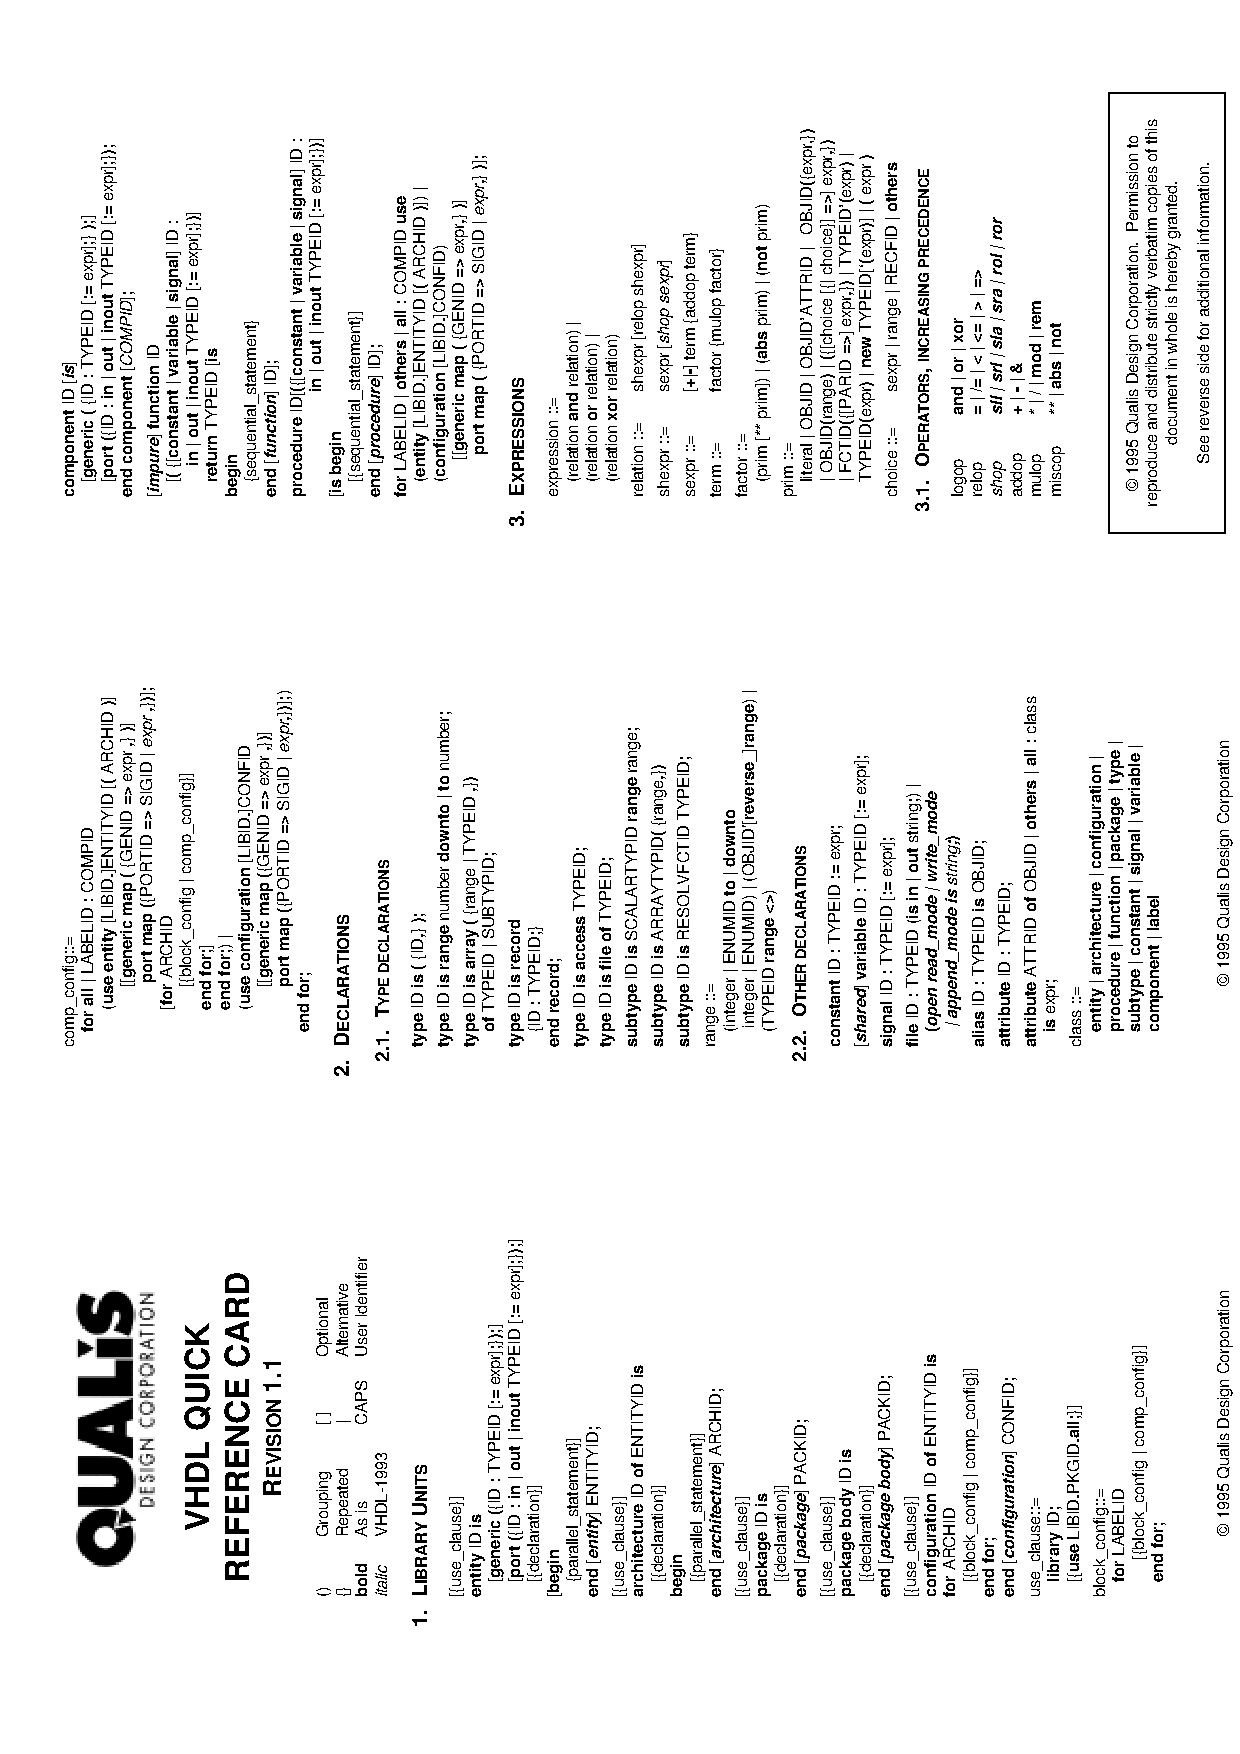
\includegraphics[width=145mm]{ref_cards/qr1.pdf}
\end{textblock*}
\null\newpage

\thispagestyle{empty}
\begin{textblock*}{148mm}(1mm,10mm)
%\textblockcolour{red}
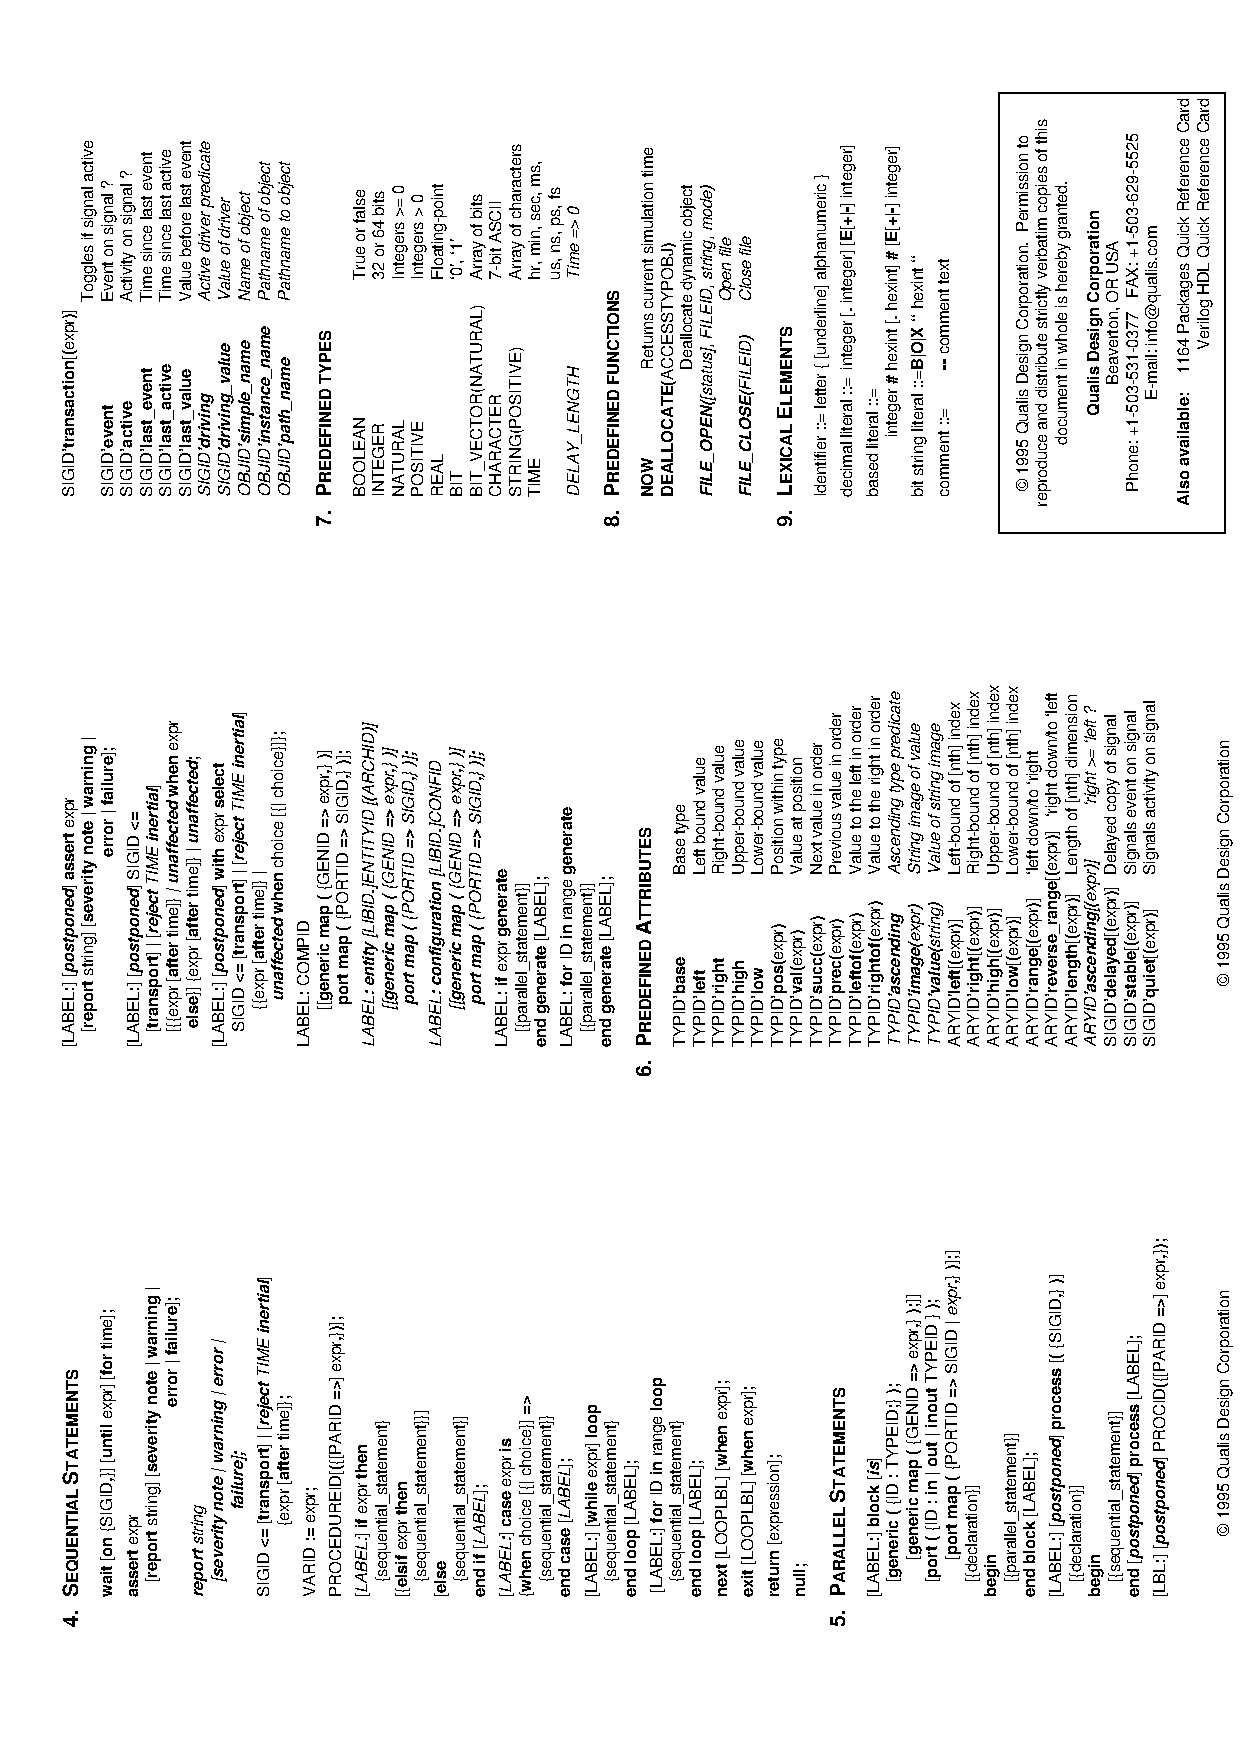
\includegraphics[width=145mm]{ref_cards/qr2.pdf}
\end{textblock*}
\null\newpage

\thispagestyle{empty}
\begin{textblock*}{148mm}(1mm,10mm)
%\textblockcolour{red}
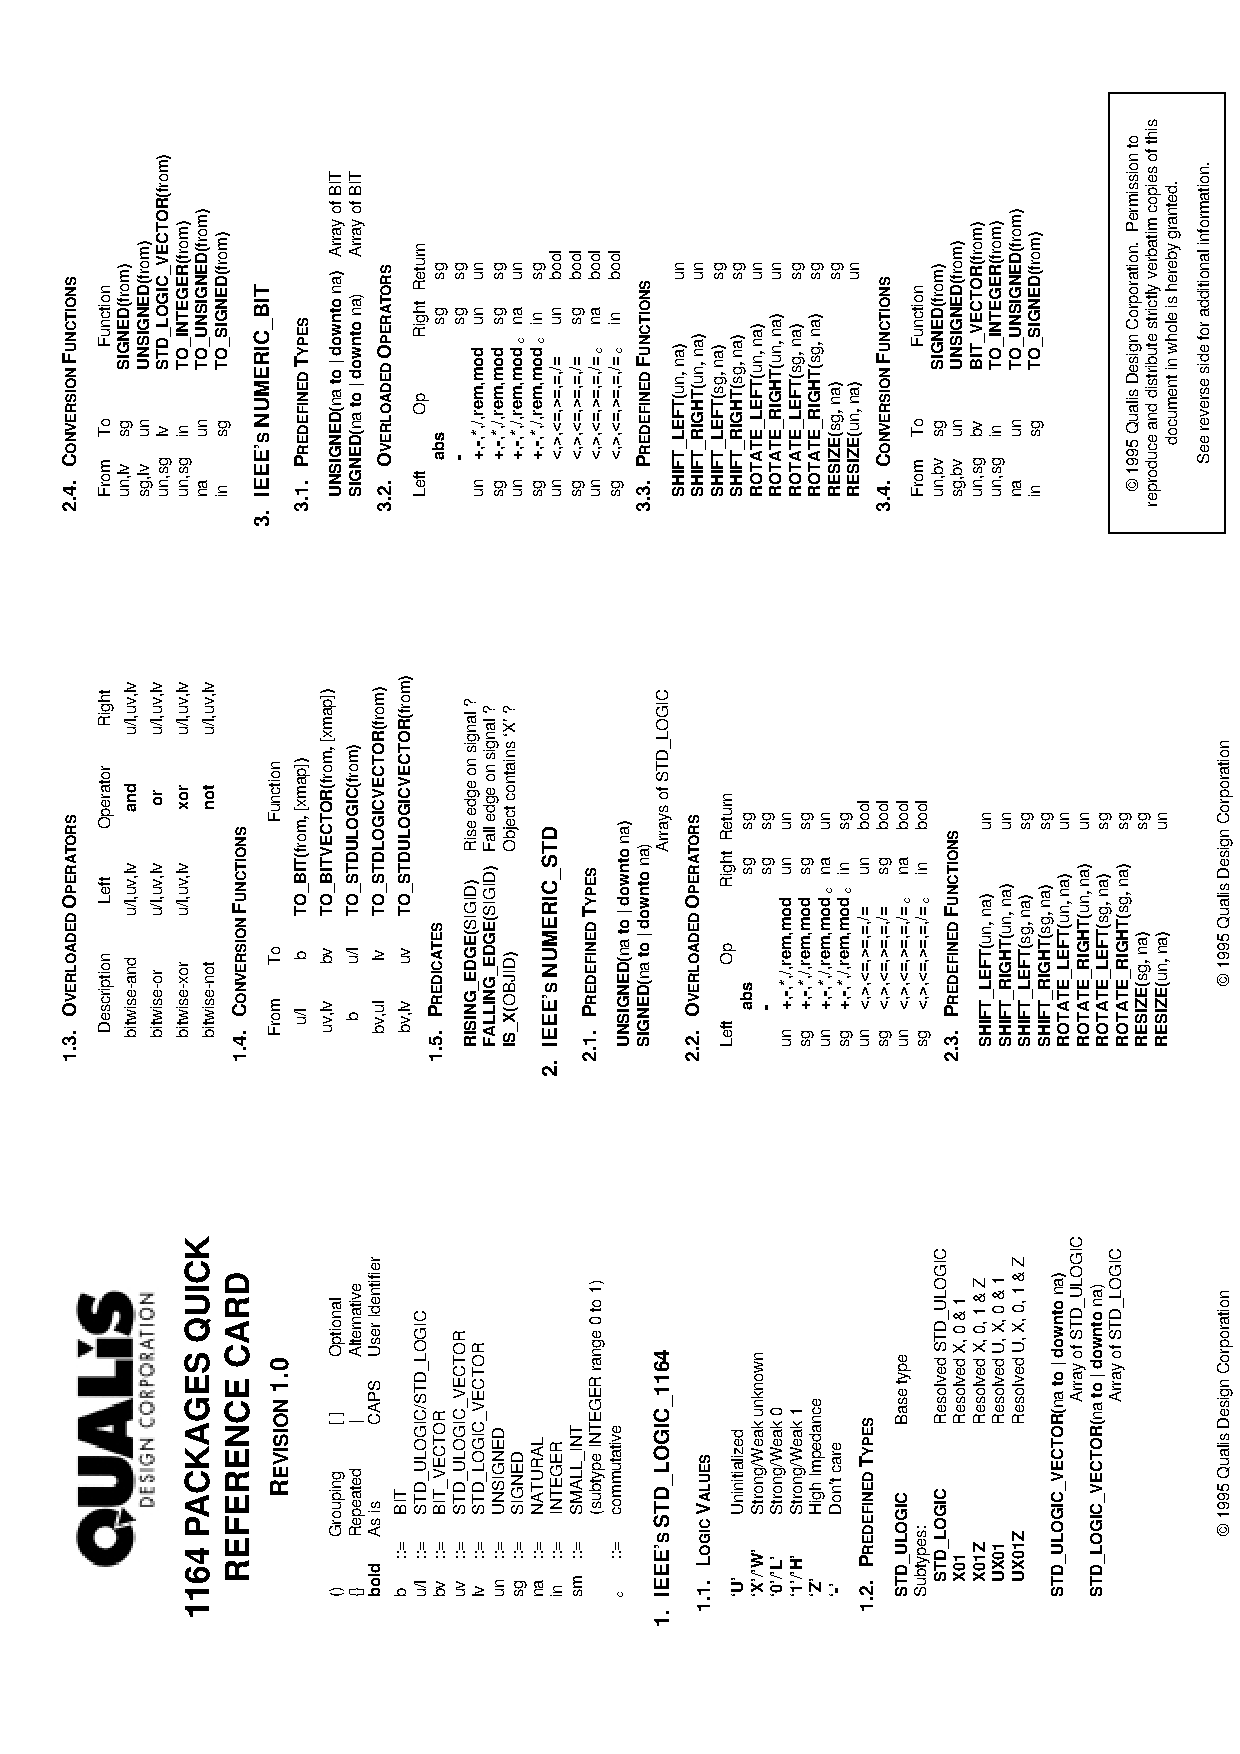
\includegraphics[width=145mm]{ref_cards/qr3.pdf}
\end{textblock*}
\null\newpage

\thispagestyle{empty}
\begin{textblock*}{148mm}(1mm,10mm)
%\textblockcolour{red}
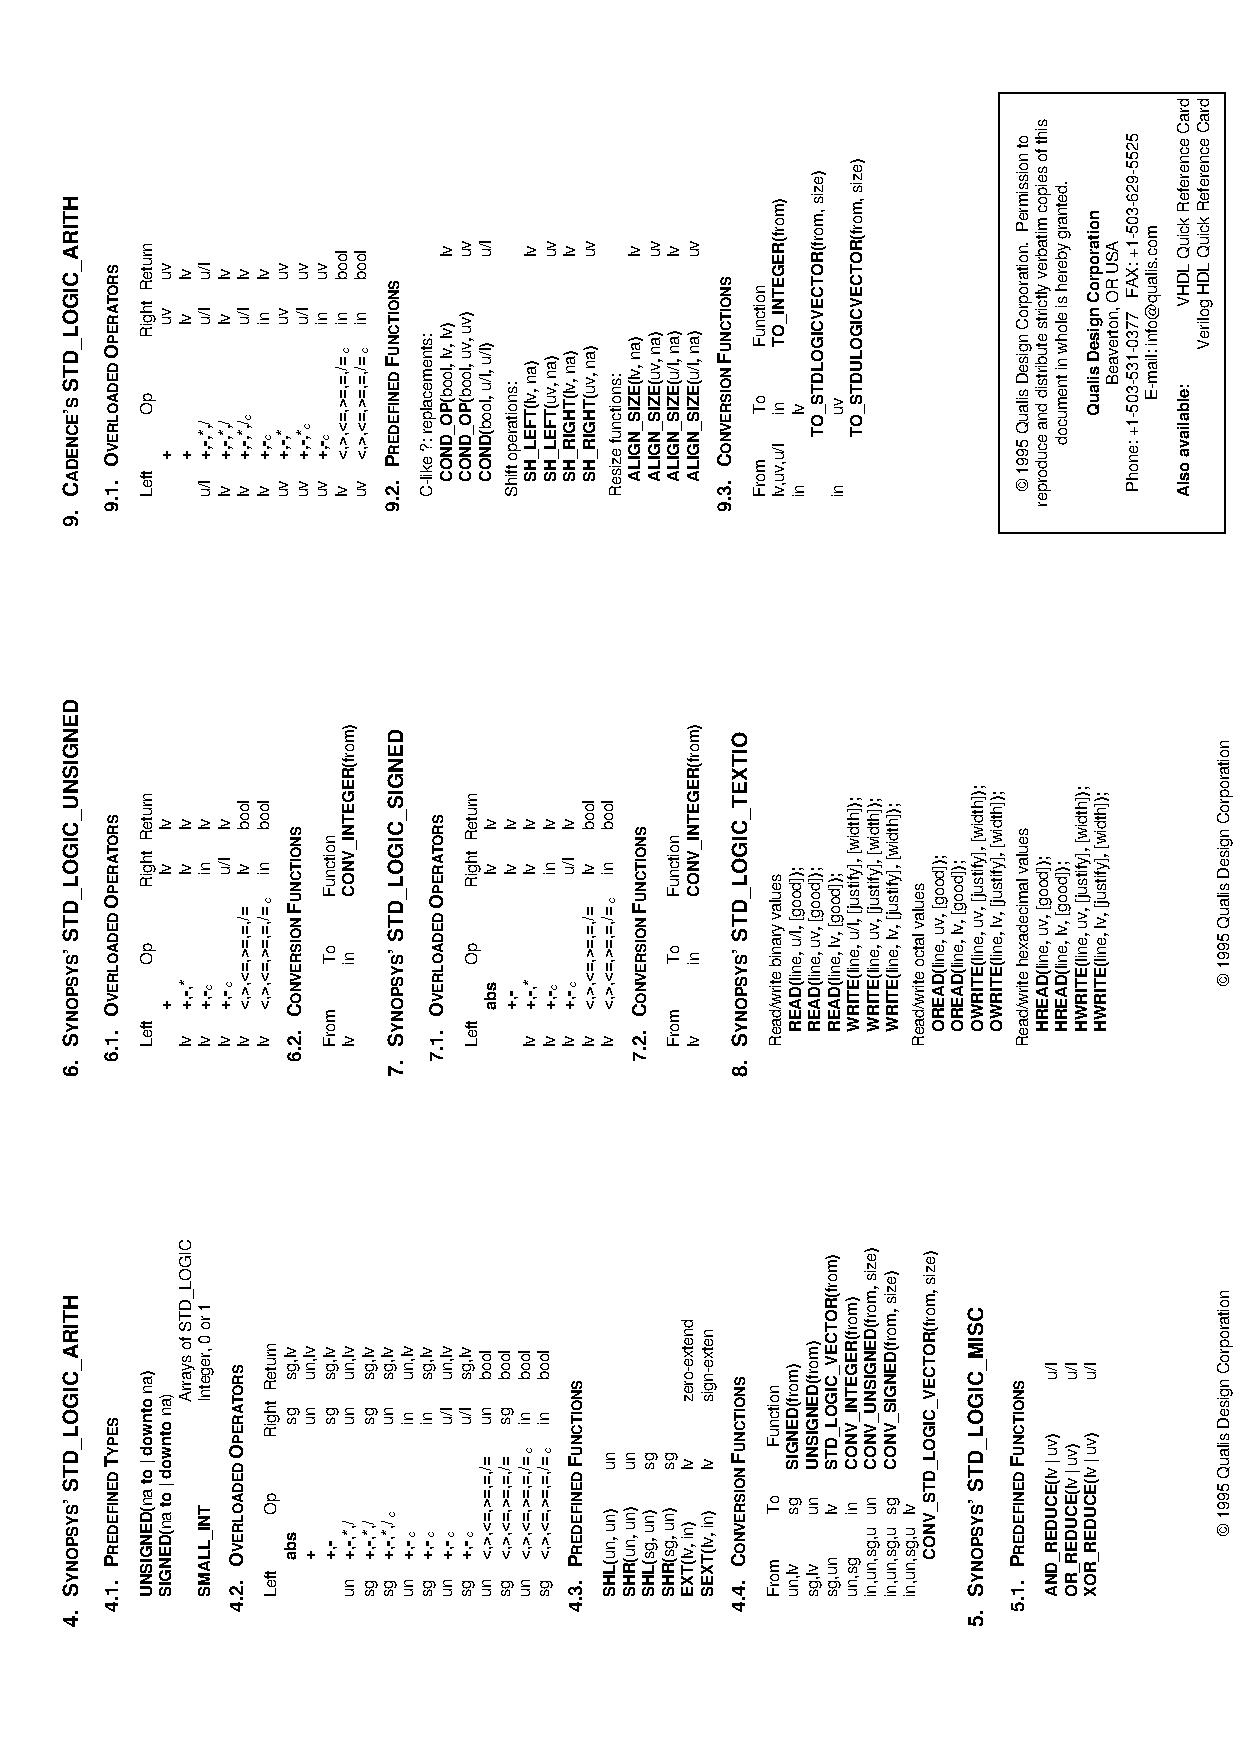
\includegraphics[width=145mm]{ref_cards/qr4.pdf}
\end{textblock*}
\null\newpage


	    % Freerange VHDL
% Authors: Bryan Mealy, Fabrizio Tappero
% Date: May, 2011
%
% (C) 2011 B. Mealy, F. Tappero
%
% !TEX root = freerange_vhdl_master.tex
%
\chapter*{Contributors of This Book}

\noindent
\textbf{Bryan Mealy} is an assistant professor at the California Polytechnic State University, San Luis Obispo, US.

\noindent
\textbf{Fabrizio Tappero} is a passionate embedded system developer with experience in academic research on satellite-based navigation systems and GNSS receiver design. Among other things, he enjoys very much coding in VHDL and Python.

\noindent
\textbf{Christina Jarron} is an Aussie technical write and editor. When she is not busy running after her customers, she spends her time wondering around the beautiful city of Barcelona. 

\noindent
\textbf{Bob Doel} is graphic designer passionate about illustrations and graphic stuff.

    \end{appendices}

    % blank page
	\thispagestyle{empty}
	\null\newpage

    % blank page
	%\thispagestyle{empty}
	%\null\newpage

\end{document}
%%%%%% DOCUMENT END  %%%%%%

